% **************************************************************************************************************
% A Classic Thesis Style
% An Homage to The Elements of Typographic Style
%
% Copyright (C) 2015 André Miede http://www.miede.de
%
% If you like the style then I would appreciate a postcard. My address 
% can be found in the file ClassicThesis.pdf. A collection of the 
% postcards I received so far is available online at 
% http://postcards.miede.de
%
% License:
% This program is free software; you can redistribute it and/or modify
% it under the terms of the GNU General Public License as published by
% the Free Software Foundation; either version 2 of the License, or
% (at your option) any later version.
%
% This program is distributed in the hope that it will be useful,
% but WITHOUT ANY WARRANTY; without even the implied warranty of
% MERCHANTABILITY or FITNESS FOR A PARTICULAR PURPOSE.  See the
% GNU General Public License for more details.
%
% You should have received a copy of the GNU General Public License
% along with this program; see the file COPYING.  If not, write to
% the Free Software Foundation, Inc., 59 Temple Place - Suite 330,
% Boston, MA 02111-1307, USA.
%
% **************************************************************************************************************
\documentclass[ twoside,openright,titlepage,numbers=noenddot,headinclude,%1headlines,% letterpaper a4paper
                footinclude=true,cleardoublepage=empty,abstractoff, % <--- obsolete, remove (todo)
                BCOR=5mm,paper=a4,fontsize=11pt,%11pt,a4paper,%
                ngerman,american,%
                ]{scrreprt}

%********************************************************************
% Note: Make all your adjustments in here
%*******************************************************
% ****************************************************************************************************
% classicthesis-config.tex 
% formerly known as loadpackages.sty, classicthesis-ldpkg.sty, and classicthesis-preamble.sty 
% Use it at the beginning of your ClassicThesis.tex, or as a LaTeX Preamble 
% in your ClassicThesis.{tex,lyx} with \input{classicthesis-config}
% ****************************************************************************************************  
% If you like the classicthesis, then I would appreciate a postcard. 
% My address can be found in the file ClassicThesis.pdf. A collection 
% of the postcards I received so far is available online at 
% http://postcards.miede.de
% ****************************************************************************************************


% ****************************************************************************************************
% 0. Set the encoding of your files. UTF-8 is the only sensible encoding nowadays. If you can't read
% äöüßáéçèê∂åëæƒÏ€ then change the encoding setting in your editor, not the line below. If your editor
% does not support utf8 use another editor!
% ****************************************************************************************************
\PassOptionsToPackage{utf8}{inputenc}
	\usepackage{inputenc}

% ****************************************************************************************************
% 1. Configure classicthesis for your needs here, e.g., remove "drafting" below 
% in order to deactivate the time-stamp on the pages
% ****************************************************************************************************
\PassOptionsToPackage{eulerchapternumbers,listings,%drafting,%
					 pdfspacing,%floatperchapter,%linedheaders,%
					 subfig,beramono,eulermath,parts}{classicthesis}                                        
% ********************************************************************
% Available options for classicthesis.sty 
% (see ClassicThesis.pdf for more information):
% drafting
% parts nochapters linedheaders
% eulerchapternumbers beramono eulermath pdfspacing minionprospacing
% tocaligned dottedtoc manychapters
% listings floatperchapter subfig
% ********************************************************************


% ****************************************************************************************************
% 2. Personal data and user ad-hoc commands
% ****************************************************************************************************
\newcommand{\myTitle}{Flexible Event Subscription\newline in Business Processes\xspace}
\newcommand{\mySubtitle}{< Any Subtitle? >\xspace}
\newcommand{\myDegree}{Ba. Sc.\xspace}
\newcommand{\myName}{Dennis Wolf\xspace}
\newcommand{\myProf}{Prof. Dr. Matthias Weske\xspace}
\newcommand{\myOtherProf}{<Other Prof>\xspace}
\newcommand{\mySupervisor}{Sankalita Mandal\xspace}
\newcommand{\myFaculty}{Digital Engineering\xspace}
\newcommand{\myDepartment}{Business Process Technology\xspace}
\newcommand{\myUni}{University of Potsdam - Hasso Plattner Institute\xspace}
\newcommand{\myLocation}{Potsdam\xspace}
\newcommand{\myTime}{August 2017\xspace}
\newcommand{\myVersion}{version 1}

% ********************************************************************
% Setup, finetuning, and useful commands
% ********************************************************************
\newcounter{dummy} % necessary for correct hyperlinks (to index, bib, etc.)
\newlength{\abcd} % for ab..z string length calculation
\providecommand{\mLyX}{L\kern-.1667em\lower.25em\hbox{Y}\kern-.125emX\@}
\newcommand{\ie}{i.\,e.}
\newcommand{\Ie}{I.\,e.}
\newcommand{\eg}{e.\,g.}
\newcommand{\Eg}{E.\,g.} 
\newcommand{\etal}{et.\,al.}
% ****************************************************************************************************


% ****************************************************************************************************
% 3. Loading some handy packages
% ****************************************************************************************************
% ******************************************************************** 
% Packages with options that might require adjustments
% ******************************************************************** 
%\PassOptionsToPackage{ngerman,american}{babel}   % change this to your language(s)
% Spanish languages need extra options in order to work with this template
%\PassOptionsToPackage{spanish,es-lcroman}{babel}
	\usepackage{babel}                  

\usepackage{csquotes}
\PassOptionsToPackage{%
    backend=biber, %instead of bibtex
	%backend=bibtex8,bibencoding=ascii,%
	language=auto,%
	style=numeric-comp,%
    %style=authoryear-comp, % Author 1999, 2010
    %bibstyle=authoryear,dashed=false, % dashed: substitute rep. author with ---
    sorting=nyt, % name, year, title
    maxbibnames=10, % default: 3, et al.
    %backref=true,%
    natbib=true % natbib compatibility mode (\citep and \citet still work)
}{biblatex}
    \usepackage{biblatex}

\PassOptionsToPackage{fleqn}{amsmath}       % math environments and more by the AMS 
    \usepackage{amsmath}

% ******************************************************************** 
% General useful packages
% ******************************************************************** 
\PassOptionsToPackage{T1}{fontenc} % T2A for cyrillics
    \usepackage{fontenc}     
\usepackage{textcomp} % fix warning with missing font shapes
\usepackage{scrhack} % fix warnings when using KOMA with listings package          
\usepackage{xspace} % to get the spacing after macros right  
\usepackage{mparhack} % get marginpar right
%\usepackage[latest]{latexrelease} % will be used once available in more distributions (ISSUE #107)
\PassOptionsToPackage{printonlyused,smaller}{acronym} 
    \usepackage{acronym} % nice macros for handling all acronyms in the thesis
    %\renewcommand{\bflabel}[1]{{#1}\hfill} % fix the list of acronyms --> no longer working
    %\renewcommand*{\acsfont}[1]{\textsc{#1}} 
    \renewcommand*{\aclabelfont}[1]{\acsfont{#1}}
% ****************************************************************************************************


% ****************************************************************************************************
% 4. Setup floats: tables, (sub)figures, and captions
% ****************************************************************************************************
\usepackage{tabularx} % better tables
    \setlength{\extrarowheight}{3pt} % increase table row height
\newcommand{\tableheadline}[1]{\multicolumn{1}{c}{\spacedlowsmallcaps{#1}}}
\newcommand{\myfloatalign}{\centering} % to be used with each float for alignment
\usepackage{caption}
% Thanks to cgnieder and Claus Lahiri
% http://tex.stackexchange.com/questions/69349/spacedlowsmallcaps-in-caption-label
% [REMOVED DUE TO OTHER PROBLEMS, SEE ISSUE #82]    
%\DeclareCaptionLabelFormat{smallcaps}{\bothIfFirst{#1}{~}\MakeTextLowercase{\textsc{#2}}}
%\captionsetup{font=small,labelformat=smallcaps} % format=hang,
\captionsetup{font=small} % format=hang,
\usepackage{subfig}  
% ****************************************************************************************************


% ****************************************************************************************************
% 5. Setup code listings
% ****************************************************************************************************
\usepackage{listings} 
%\lstset{emph={trueIndex,root},emphstyle=\color{BlueViolet}}%\underbar} % for special keywords
\lstset{language=[LaTeX]Tex,%C++,
    morekeywords={PassOptionsToPackage,selectlanguage},
    keywordstyle=\color{RoyalBlue},%\bfseries,
    basicstyle=\small\ttfamily,
    %identifierstyle=\color{NavyBlue},
    commentstyle=\color{Green}\ttfamily,
    stringstyle=\rmfamily,
    numbers=none,%left,%
    numberstyle=\scriptsize,%\tiny
    stepnumber=5,
    numbersep=8pt,
    showstringspaces=false,
    breaklines=true,
    %frameround=ftff,
    %frame=single,
    belowcaptionskip=.75\baselineskip
    %frame=L
} 
% ****************************************************************************************************             


% ****************************************************************************************************
% 6. PDFLaTeX, hyperreferences and citation backreferences
% ****************************************************************************************************
% ********************************************************************
% Using PDFLaTeX
% ********************************************************************
\PassOptionsToPackage{pdftex,hyperfootnotes=false,pdfpagelabels}{hyperref}
    \usepackage{hyperref}  % backref linktocpage pagebackref
\pdfcompresslevel=9
\pdfadjustspacing=1 
\PassOptionsToPackage{pdftex}{graphicx}
    \usepackage{graphicx} 
 

% ********************************************************************
% Hyperreferences
% ********************************************************************
\hypersetup{%
    %draft, % = no hyperlinking at all (useful in b/w printouts)
    colorlinks=true, linktocpage=true, pdfstartpage=3, pdfstartview=FitV,%
    % uncomment the following line if you want to have black links (e.g., for printing)
    %colorlinks=false, linktocpage=false, pdfstartpage=3, pdfstartview=FitV, pdfborder={0 0 0},%
    breaklinks=true, pdfpagemode=UseNone, pageanchor=true, pdfpagemode=UseOutlines,%
    plainpages=false, bookmarksnumbered, bookmarksopen=true, bookmarksopenlevel=1,%
    hypertexnames=true, pdfhighlight=/O,%nesting=true,%frenchlinks,%
    urlcolor=webbrown, linkcolor=RoyalBlue, citecolor=webgreen, %pagecolor=RoyalBlue,%
    %urlcolor=Black, linkcolor=Black, citecolor=Black, %pagecolor=Black,%
    pdftitle={\myTitle},%
    pdfauthor={\textcopyright\ \myName, \myUni, \myFaculty},%
    pdfsubject={},%
    pdfkeywords={},%
    pdfcreator={pdfLaTeX},%
    pdfproducer={LaTeX with hyperref and classicthesis}%
}   

% ********************************************************************
% Setup autoreferences
% ********************************************************************
% There are some issues regarding autorefnames
% http://www.ureader.de/msg/136221647.aspx
% http://www.tex.ac.uk/cgi-bin/texfaq2html?label=latexwords
% you have to redefine the makros for the 
% language you use, e.g., american, ngerman
% (as chosen when loading babel/AtBeginDocument)
% ********************************************************************
\makeatletter
\@ifpackageloaded{babel}%
    {%
       \addto\extrasamerican{%
			\renewcommand*{\figureautorefname}{Figure}%
			\renewcommand*{\tableautorefname}{Table}%
			\renewcommand*{\partautorefname}{Part}%
			\renewcommand*{\chapterautorefname}{Chapter}%
			\renewcommand*{\sectionautorefname}{Section}%
			\renewcommand*{\subsectionautorefname}{Section}%
			\renewcommand*{\subsubsectionautorefname}{Section}%     
                }%
       \addto\extrasngerman{% 
			\renewcommand*{\paragraphautorefname}{Absatz}%
			\renewcommand*{\subparagraphautorefname}{Unterabsatz}%
			\renewcommand*{\footnoteautorefname}{Fu\"snote}%
			\renewcommand*{\FancyVerbLineautorefname}{Zeile}%
			\renewcommand*{\theoremautorefname}{Theorem}%
			\renewcommand*{\appendixautorefname}{Anhang}%
			\renewcommand*{\equationautorefname}{Gleichung}%        
			\renewcommand*{\itemautorefname}{Punkt}%
                }%  
            % Fix to getting autorefs for subfigures right (thanks to Belinda Vogt for changing the definition)
            \providecommand{\subfigureautorefname}{\figureautorefname}%             
    }{\relax}
\makeatother


% ****************************************************************************************************
% 7. Last calls before the bar closes
% ****************************************************************************************************
% ********************************************************************
% Development Stuff
% ********************************************************************
\listfiles
%\PassOptionsToPackage{l2tabu,orthodox,abort}{nag}
%   \usepackage{nag}
%\PassOptionsToPackage{warning, all}{onlyamsmath}
%   \usepackage{onlyamsmath}

% ********************************************************************
% Last, but not least...
% ********************************************************************
\usepackage{classicthesis} 
% ****************************************************************************************************


% ****************************************************************************************************
% 8. Further adjustments (experimental)
% ****************************************************************************************************
% ********************************************************************
% Changing the text area
% ********************************************************************
%\linespread{1.05} % a bit more for Palatino
%\areaset[current]{312pt}{761pt} % 686 (factor 2.2) + 33 head + 42 head \the\footskip
%\setlength{\marginparwidth}{7em}%
%\setlength{\marginparsep}{2em}%

% ********************************************************************
% Using different fonts
% ********************************************************************
%\usepackage[oldstylenums]{kpfonts} % oldstyle notextcomp
%\usepackage[osf]{libertine}
%\usepackage[light,condensed,math]{iwona}
%\renewcommand{\sfdefault}{iwona}
%\usepackage{lmodern} % <-- no osf support :-(
%\usepackage{cfr-lm} % 
%\usepackage[urw-garamond]{mathdesign} <-- no osf support :-(
%\usepackage[default,osfigures]{opensans} % scale=0.95 
%\usepackage[sfdefault]{FiraSans}
% ****************************************************************************************************

% my custom packages
\usepackage[]{todonotes}
\usepackage{array}


%********************************************************************
% Bibliographies
%*******************************************************
\addbibresource{bibliography.bib}

%********************************************************************
% Hyphenation
%*******************************************************
%\hyphenation{put special hyphenation here}

\begin{document}
\frenchspacing
\raggedbottom
\selectlanguage{american} % american ngerman
%\renewcommand*{\bibname}{new name}
%\setbibpreamble{}
\pagenumbering{roman}
\pagestyle{plain}
%********************************************************************
% Frontmatter
%*******************************************************
%%*******************************************************
% Little Dirty Titlepage
%*******************************************************
\thispagestyle{empty}
%\pdfbookmark[1]{Titel}{title}
%*******************************************************
\begin{center}
    \spacedlowsmallcaps{\myName} \\ \medskip                        

    \begingroup
        \color{Maroon}\spacedallcaps{\myTitle}
    \endgroup
\end{center}        

%*******************************************************
% Titlepage
%*******************************************************
\begin{titlepage}
    % if you want the titlepage to be centered, uncomment and fine-tune the line below (KOMA classes environment)
    \begin{addmargin}[-1cm]{-3cm}
    \begin{center}
        \large  

        \hfill

        \vfill

        \begingroup
            \color{Maroon}\spacedallcaps{\myTitle} \\ \bigskip
        \endgroup

        \spacedlowsmallcaps{\myName}

        \vfill

        
\includegraphics[width=6cm]{frontbackmatter/gfx/hpi_logo.jpg} \\ \medskip

        %\mySubtitle \\ \medskip   
        %\myDegree \\
        \myDepartment \\                            
        %\myFaculty \\
        \myUni \\ \bigskip
        

        Handed in \myTime\ % -- \myVersion

        \vfill                      

    \end{center}  
  \end{addmargin}       
\end{titlepage}   
\thispagestyle{empty}

\hfill

\vfill

\noindent\myName: \textit{\myTitle,} \mySubtitle, %\myDegree, 
\textcopyright\ \myTime

%\bigskip
%
%\noindent\spacedlowsmallcaps{Supervisors}: \\
%\myProf \\
%\myOtherProf \\ 
%\mySupervisor
%
%\medskip
%
%\noindent\spacedlowsmallcaps{Location}: \\
%\myLocation
%
%\medskip
%
%\noindent\spacedlowsmallcaps{Time Frame}: \\
%\myTime

\cleardoublepage%*******************************************************
% Abstract
%*******************************************************
%\renewcommand{\abstractname}{Abstract}
\pdfbookmark[1]{Abstract}{Abstract}
\begingroup
\let\clearpage\relax
\let\cleardoublepage\relax
\let\cleardoublepage\relax

\chapter*{Abstract}
Business process models have become an essential tool in organizing, documenting and executing company work flows while Event Processing can be used as a powerful tool to increase their flexibility especially in distributed scenarios. 
The publish-subscribe paradigm is commonly used when communicating with complex event processing platforms, nevertheless prominent process modeling notations do not specify how to handle event subscription.

At the example of BPMN 2.0, the first part of this work illustrates the need for a flexible event subscription time in process models and derives new requirements for process modeling notations. An assessment of the coverage of these requirements in BPMN 2.0 is presented and shortcomings are pointed out.

Based on the identified requirements, this work presents a new concept for handling event subscription in business process management solutions, predominantly built on the notion of event buffers. The concept includes an extension to the BPMN meta model, specifies the semantics and API of a new event buffering module and describes the changes necessary to the behavior of the process engine.

For evaluation purposes, the concept has been implemented as a reusable Camunda Process Engine Plugin that interacts with the academic Complex Event Processing Platform UNICORN.

\pagebreak
\vfill


\begin{otherlanguage}{ngerman}
\pdfbookmark[1]{Zusammenfassung}{Zusammenfassung}
\chapter*{Zusammenfassung}

Im heutigen Unternehmensumfeld sind Geschäftsprozessmodelle ein anerkanntes Werkzeug um Arbeitsabläufe zu organisieren, zu dokumentieren und automatisiert auszuführen. \acf{CEP} kann dabei verwendet werden um die Flexiblität und Effizienz der Prozesse zu verbessern.
Die Kommunikation mit CEP Plattformen folgt dabei dem publish-subscribe Muster, allerdings wird es von den wichtigsten Prozessmodellierungssprachen bisher nicht explizit beachtet.

Am Beispiel von BPMN 2.0 wird in dieser Arbeit zuerst der Bedarf nach einer flexiblen Nutzung von Event subscription erläutert, wovon konkrete Anforderungen an Modellierungsstandards abgeleitet werden. Es wird im Anschluss untersucht, inwiefern diese Anforderungen in BPMN untersützt sind, woraufhin zusätzliche Mängel ausgearbeitet werden.

Auf Basis dieser erweiterten Anforderungen wird anschließend eine Erweiterung zum BPMN Meta Model präsentiert, welche die Modellierung der subscribe-Operationen in Geschäftsprozessen ermöglicht. Dabei ist besonderer Wert auf den Zeitpunkt des Abonnierens gelegt, um den erarbeiteten Anforderungen gerecht zu werden.
Zur Evaluierung des Konzepts wird zuletzt eine Referenzimplementierung unter Nutzung von Camunda und Unicorn vorgestellt.


\end{otherlanguage}

\endgroup			

\vfill
\pagestyle{scrheadings}
\cleardoublepage%*******************************************************
% Table of Contents
%*******************************************************
%\phantomsection
\refstepcounter{dummy}
\pdfbookmark[1]{\contentsname}{tableofcontents}
\setcounter{tocdepth}{2} % <-- 2 includes up to subsections in the ToC
\setcounter{secnumdepth}{3} % <-- 3 numbers up to subsubsections
\manualmark
\markboth{\spacedlowsmallcaps{\contentsname}}{\spacedlowsmallcaps{\contentsname}}
\tableofcontents 
\automark[section]{chapter}
\renewcommand{\chaptermark}[1]{\markboth{\spacedlowsmallcaps{#1}}{\spacedlowsmallcaps{#1}}}
\renewcommand{\sectionmark}[1]{\markright{\thesection\enspace\spacedlowsmallcaps{#1}}}
%*******************************************************
% List of Figures and of the Tables
%*******************************************************
\clearpage

\begingroup 
    \let\clearpage\relax
    \let\cleardoublepage\relax
    \let\cleardoublepage\relax
    %*******************************************************
    % List of Figures
    %*******************************************************    
    %\phantomsection 
    \refstepcounter{dummy}
    %\addcontentsline{toc}{chapter}{\listfigurename}
    \pdfbookmark[1]{\listfigurename}{lof}
    \listoffigures

    \vspace{8ex}

    %*******************************************************
    % List of Tables
    %*******************************************************
    %\phantomsection 
    \refstepcounter{dummy}
    %\addcontentsline{toc}{chapter}{\listtablename}
    \pdfbookmark[1]{\listtablename}{lot}
    \listoftables
    \todo[inline]{Do I need a list of tables?}
        
    \vspace{8ex}
%   \newpage
    
    %*******************************************************
    % List of Listings
    %*******************************************************      
      %\phantomsection 
    \refstepcounter{dummy}
    %\addcontentsline{toc}{chapter}{\lstlistlistingname}
    \pdfbookmark[1]{\lstlistlistingname}{lol}
    \lstlistoflistings 

    \vspace{8ex}
       
    %*******************************************************
    % Acronyms
    %*******************************************************
    %\phantomsection 
    \refstepcounter{dummy}
    \pdfbookmark[1]{Acronyms}{acronyms}
    \markboth{\spacedlowsmallcaps{Acronyms}}{\spacedlowsmallcaps{Acronyms}}
    \chapter*{Acronyms}
    \begin{acronym}[UMLX]
        \acro{API}{Application Programming Interface}
        \acro{BPM}{Business Process Management}
        \acro{BPMN}{Business Process Model and Notation}
        \acro{CEP}{Complex Event Processing}
        \acro{EdBPM}{Event-driven Business Process Management}
        \acro{EPL}{Event Processing Language}
        \acro{JVM}{Java Virtual Machine}
        \acro{HTTP}{Hypertext Transfer Protocol}
        \acro{PEP}{Process Engine Plugin}
        \acro{REST}{Respresentational State Transfer}
        \acro{SQL}{Structured Query Language}
        \acro{UML}{Unified Modeling Language}
        \acro{XML}{Extensible Markup Language}
    \end{acronym}                     
\endgroup

%********************************************************************
% Mainmatter
%*******************************************************
\cleardoublepage\pagenumbering{arabic}
%\setcounter{page}{90}
% use \cleardoublepage here to avoid problems with pdfbookmark
\cleardoublepage
%\ctparttext{You can put some informational part preamble text here.}
%\part{Some Kind of Manual}
%************************************************
\chapter{Introduction}
%************************************************

Given the increasing competition on the global market place, companies are seeking to improve their products while reducing costs.
In many areas, \ac{BPM} has been chosen as one of the tools to help stay competitive.
Especially large enterprises, but also small to medium businesses formalize their work-flows in business process models to allow their automatized execution and management, archiving and documentation.

% maybe a little more on BPM?

With Business Process Technology in constant progression, the opportunities that the field has to offer are ever growing.
Since the recent years, many efforts have been dedicated towards bringing together business processes and \ac{CEP}.
By the help of event processing systems, companies are trying to get a hold of the exponentially growing amounts of data that occur in today's IT~environment.
Event Engines are designed to process thousands of events each second while supporting the integration of multiple event types and sources to derive new information.
%Therefor, incoming data is evaluated according to query expressions, themselves producing new, enhanced events.% by projection, filtering, aggregating or joining.
By having conglomerated information available almost in real-time, companies can react quickly on complex situations within their organization or anywhere on the world.
The connection of events and business processes has developed into an own discipline, \acl{EdBPM}, which is performed from two perspectives.
%- 2 variants of doing edbpm
%https://www.researchgate.net/profile/Oliver_Mueller5/publication/241635758_Extending_BPMN_for_Business_Activity_Monitoring/links/0deec52d00ef9276c9000000.pdf
%(BAM) refers to the observation, analysis, and presentation of real-time information about business activities across systems’ and companies’ borders.
During execution, business processes can take the role of an event producer and publish information about their status, errors or incidents. 
Processed through complex event processing, this information can be utilized for business activity monitoring which aims at providing timeliness and effectiveness of operational business processes.
In a second field of research, processes consume events so that the projected work-flow can be influenced and controlled.
By that means, events heavily increase the capabilities and flexibility in process flows. They can enable intra-organizational communication between processes or business departments, but also allow to respond to external situations within seconds and milliseconds.

The \ac{BPMN}, the most prominent industry standard for representing business processes,% both visually and through a textual model, 
natively supports the use of events in numerous fashions. Event-related elements are a main building block of the modeling language and can, for instance, be used for instantiating processes, communicating between process participants or to support decisions.
Thereby, event-driven process control combines the advantages of \acl{BPM} and Complex Event Processing.


\section{Motivation}

An interaction with a Complex Event Processing platform generally follows the publish-subscribe paradigm: The event consumer contacts the platform and issues a subscription to a specific subset of available events.
The event producer, for example a vehicle providing its current GPS location, publishes information to the event processing platform, which is then forwarded to every consumer that had subscribed.
As event processing has become an essential part of \ac{BPM}, there is a need for the available modeling frameworks to consider these interaction patterns.

This work investigates the aspect at the example of the \ac{BPMN}, where \textit{Intermediate Events} enable event-based process control between the start and the end of a process. %and hence facilitate the consumption of complex events. %reception of external message events.
However, the BPMN specification does not specifically consider the publish-subscribe work-flow and consequently provides only limited capabilities to represent event subscription and un-subscription operations in business process models.
From the execution semantics of intermediate events, the common interpretation is that the subscription to an event source implicitly happens when an event is enabled, the un-subscription on termination of the element~(see~\cite{} re-eval, mandal, earlier paper).
- mandal add the idea of issuing subscriptions explicitly through a customized service task.
%- while other work on the use of complex events does not mention subscription and un-subscription at all
% > probably assuming that a subscription is already active
%- there is research on including the subscription query in the model, but the subscription time is not further defined
Given that the subscription to an event must take place strictly before consumption, the time to listen to an event is limited to only a segment of the process execution.
Naturally, in event processing, a large number of participants can be involved to cause a complex event. This high level of distribution and the inclusion of external sources implies that the time of event occurrence cannot be entirely controlled.

As defined in the BPMN specification, an intermediate catch event will wait for the associated event to occur. In case the event does not occur or only after a significant amount of time, this behavior leads to a delay or even a complete halt of the process execution. %reduce process efficiency
While some process designs require just these semantics, in others they cause an unnecessary reduction of efficiency and reliability.%the variable time of event occurrence
\todo[inline]{short example, maybe harvesting?}
This behavior is further illustrated by the help of two example scenarios in \autoref{ch:motivatingexamples}.
An earlier subscription to an event source would increase the timespan in that events can be received and thus reduce the probability of missing events.
This motivates the investigation of mechanisms to more flexibly incorporate subscribe operations in business processes.
% also definition of subscription stuff in general, because there is no standard.

%The ability to influence the event subscription time more flexibly 
%- to ensure the efficient use of events in processes, a more flexible use of subscription is necessary
%- that implies the additional need for buffers
%This work investigates the consequences of this lack of specification and provides a design and implementation to overcome the identified shortcomings.

\section{Contribution \& Structure}
Aiming towards the extension of the BPMN modeling standard for the flexible use of event subscription, this thesis provides three main contributions:
%(1) requirements through ? + shortcomings from assessment of the capabilities of standard bpmn
(1)~From the analysis of motivating scenarios and the current state of research, an initial set of requirements~(\autoref{ch:requirements}) is derived in the course of \autoref{ch:problemstatement} and evaluated against current BPM solutions in \autoref{ch:assessment}.
The requirements define the functionality necessary for representing event subscription mechanisms in business processes models. 
They are supplemented by a list of shortcomings of BPMN~(\autoref{ch:ass:discussion}), which yields from the assessment of its meta model against the specified requirements.

%Their assessment results in an additional list of shortcomings of , which is obtained by evaluating current BPM solutions% and the Camunda business process engine %against the requirements. %together, they form the foundation for...
%and derives a set of requirements that a business process meta model must fulfill to enable the inclusion of subscription operations in the model and also to allow influencing the time of subscription
%in the course of this assessment, an additional set of shortcomings is identified

% (2) Proposition of a BPMN extension for flexible event subscription, its advantages and derived requirements to process engines and CEP platforms
(2)~Based on the requirements and identified shortcomings of current solutions, \autoref{ch:flexibleeventsubscription} presents an extension to the notation and meta model of the BPMN including an XML-specification and a description of the expected execution semantics. 
The extension enables the incorporation of subscription-related information in the process model, allowing to flexibly chose the time of event subscription~(\autoref{ch:bpmnx}).
The concept hides the necessary underlying infrastructure tasks from the model by requiring automatic subscription handling within the process engine.
A reference architecture stating the changes necessary to the behavior of the process engine and the event processing module is presented in \autoref{ch:automaticsubscription}. %automatic subscription handling

%Event buffers are an essential part of the concept

% (3) A reference implementation using Camunda and UNICORN
(3)~Finally, \autoref{ch:implementation} evaluates the presented concept through a reference implementation at the example of the Camunda business process engine and the Unicorn event processing platform.
The resulting BPM system is capable of handling the extended BPMN process models, automatically handling event subscription, un-subscrption and event buffering.



\cleardoublepage%************************************************
\chapter{Background on Event-Driven Business Process Management}\label{ch:background}
%************************************************

\section{Business Process Management}\label{ch:bg:bpm}
With its origins dating back to the process orientation trend of the 1990s, \ac{BPM} has meanwhile become a mainstream tool to support organizations.
It had been noted, that company workflows can essentially be broken down into activities that are executed in a coordinated manner by one or more parties.
A certain group of activities thereby form a process which is executed within an organization.
More precisely, \citeauthor{weske:bpm-book} \cite{weske:bpm-book} defines a single \emph{business process} as follows:

\begin{description}
	\item[Definition 1 (Business Process):]
	A \emph{business process} consists of a set of activities that are performed in coordination to realize a business goal. Each business process is enacted by a single organization, but it may interact with processes performed by other organizations.
\end{description}

\noindent The term \emph{Business process management} describes the techniques available to develop and support processes throughout their life-cycle.
It is grounded in the use of explicit process representations which ultimately allow the exchange, analysis and reproduction of the workflows.
This process specification is referred to as the \emph{business process model}, composed mainly of activities and the rules that are necessary to coordinate their execution.
When a process is performed according to its model, the single execution is called \textit{process instance}.
Based on a process model, the number of possible instances is theoretically unbounded.

\begin{description}
	\item[Definition 2 (Business Process Model):]
	A \emph{business process model} consists of a set of activity models and execution constraints between them. A \emph{business process instance} represents a concrete case in the operational business of a company, consisting of activity instances.
	\cite[p.~7]{weske:bpm-book}
\end{description}

\noindent
The life-cycle of a business process can be described by four phases in that numerous stakeholders interact and contribute depending on their specialization.
Process development starts with a \emph{Design~\&~Analysis} phase which yields a refined and validated business process model.
In the following \emph{Configuration} phase, it is necessary to prepare the process implementation, select the means and an environment to run the process in.
The action of making the process runnable in the execution environment is called \emph{process deployment}.
After these preparations the process can be enacted in daily business while its current state is monitored and system maintenance is performed if necessary (\emph{Enactment Phase}). 
A single process execution begins with the \emph{process instantiation}, when the process has succeeded or is aborted, we say the process is \emph{terminated}.
During the enactment, system and stakeholders can start collecting performance indicators and process execution logs to allow evaluating the quality of the process specification. If that \emph{Evaluation} step reveals deficiencies, the life-cycle starts over by entering the design phase once again.
The \emph{process un-deployment} is performed if necessary, so that no new instances of the old process can be started~\cite[p.~11~ff.]{weske:bpm-book}. A similar life-cycle is described by Dumas in \cite{dumas:bpm}.
%\todo[inline]{add reference to \cite{dumas:bpm}, mention that Weske says pretty much the same}
%the investigations undertaken in this work target the Design \& Analysis phase

While traditionally activities are executed manually by company staff following the written process specifications, computer systems are used today to drive the execution and enforcement of business processes and organizational rules.
The generic software systems utilized for that purpose are introduced in the following section.

\subsection{Business Process Management Systems}\label{ch:bg:bpms}
The implementation of business processes has developed from a manual execution guided by business rules to a fully automatized execution in a specialized IT environment.
One of the main reasons for \acs{BPM}'s growing popularity is that in today's fast-paced economy, a large part of the business activity is either supported by computers or even carried out autonomously by them.
The specialized software systems that are utilized to support the enactment of business processes are referred to as \emph{business process management systems}.

\paragraph{Process Management Architecture}
A typical IT infrastructure for driving business processes is illustrated in \autoref{fig:bpm-architecture}. 
Five principal building blocks are considered which will be explained in the following.

With reference to the business process lifecycle, the visualized scenario commences with the \emph{Business Process Modeling}. As a result of the \emph{Design \& Analysis} phase, new process models are created and refined to be stored in the \emph{Business Process Model Repository}. 
The relation between the two elements includes writing new models to the repository as well as reading models for review and further modification.
Given that the desired model is approved for enactment, the process gets deployed to the \emph{Process Engine} as part of the configuration step.
The process engine is the heart of the execution environment. It performs the execution of the processes from deployment until un-deployment, while the enactment and instantiation is controlled by the \emph{Business Process Environment}.
An indefinite number of \emph{Service Provider}s realize application services to support the process execution. A service provider can be a software module but also a knowledge worker performing a particular process step.

\begin{figure}[]
	\myfloatalign
	{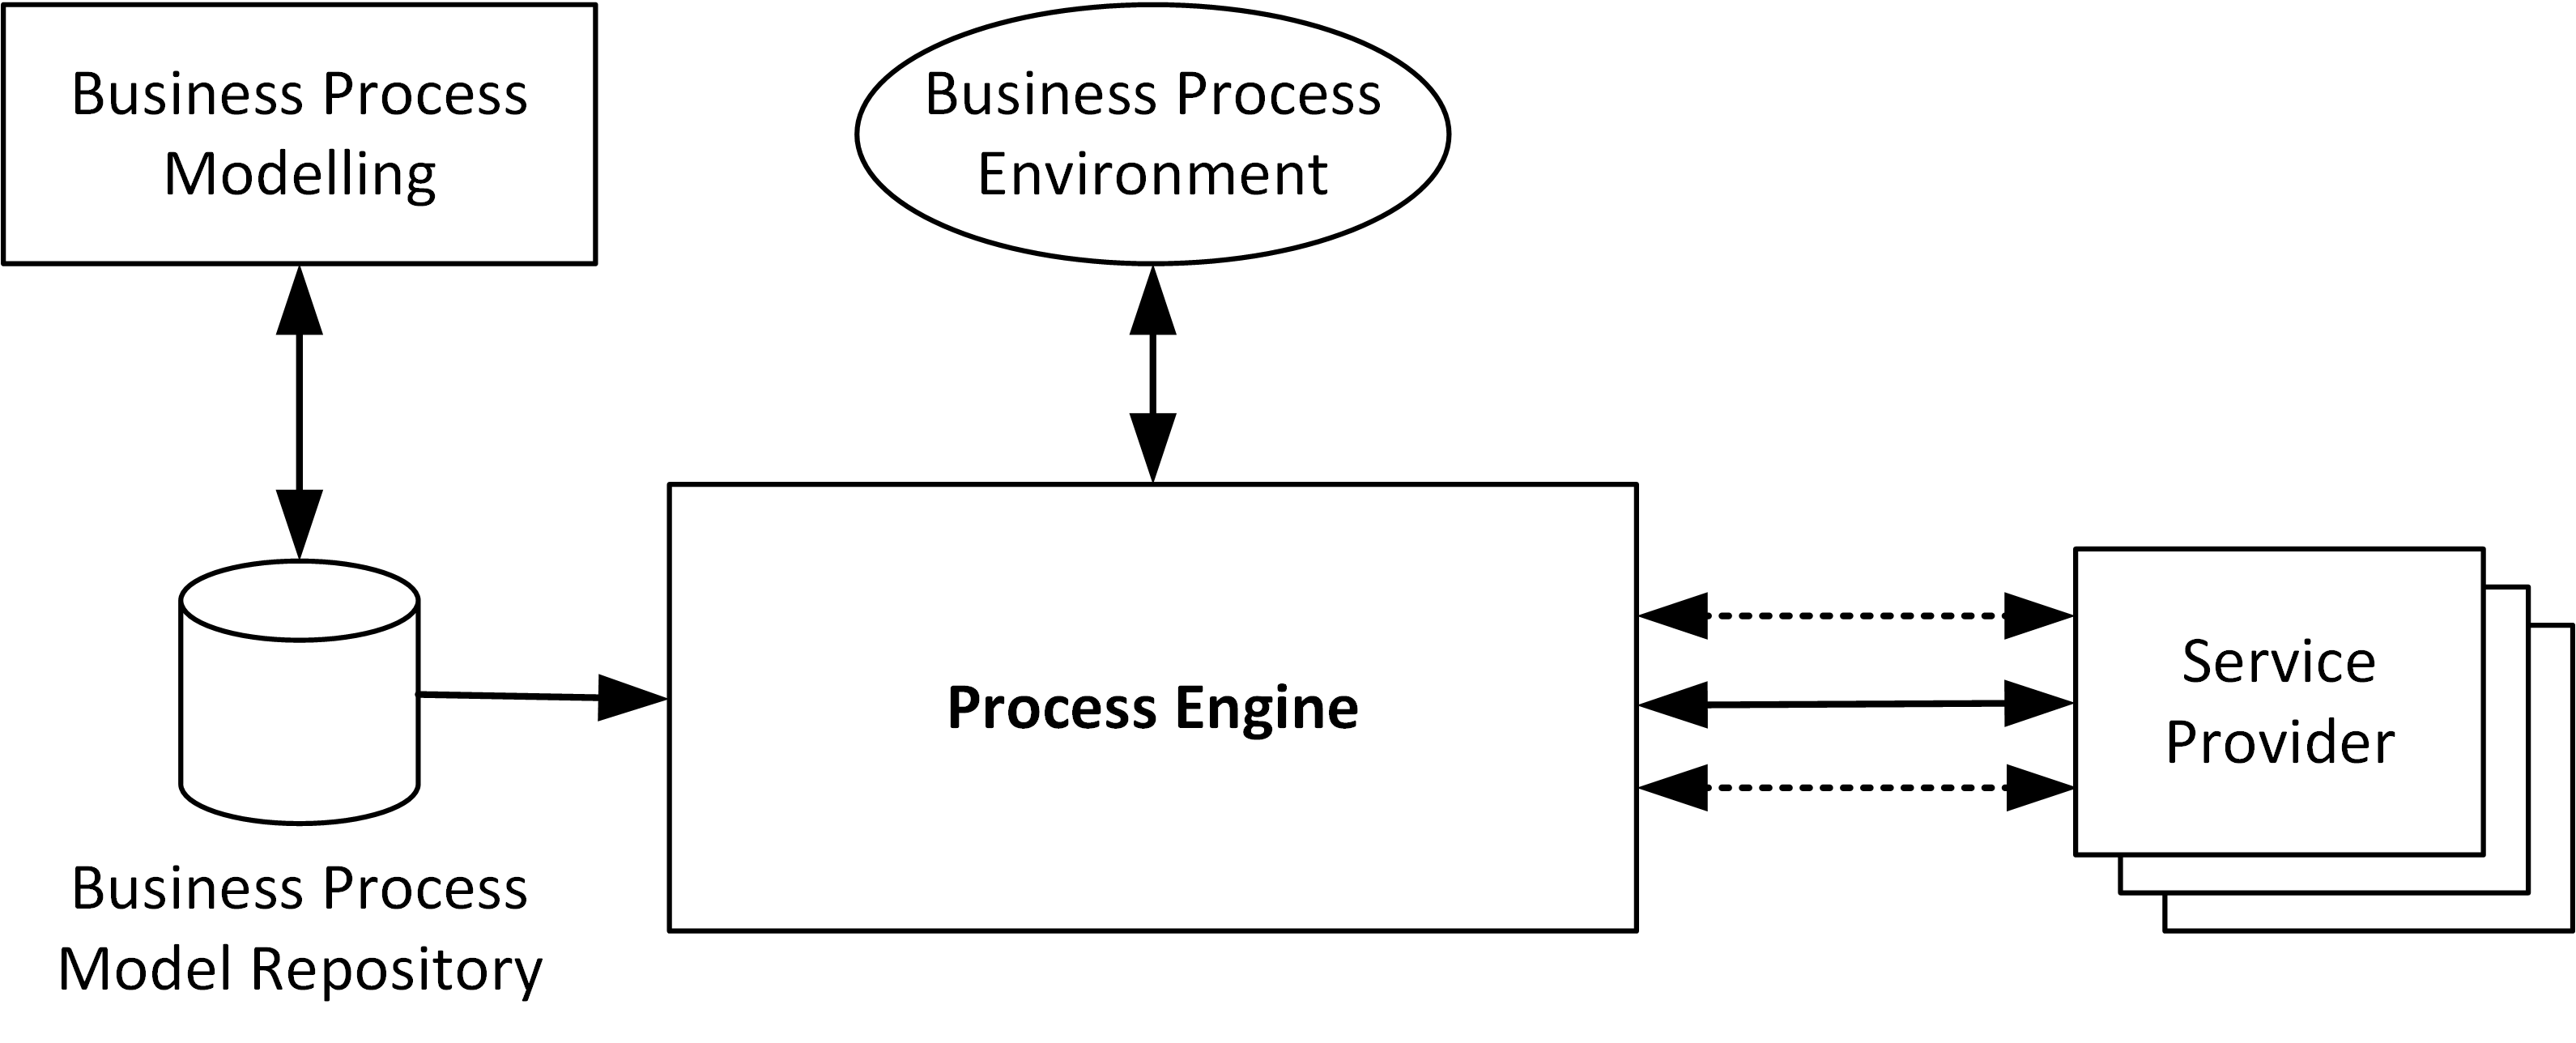
\includegraphics[width=1\linewidth]{chapters/background/bpm-architecture.png}}
	\caption{Business process management systems architecture model (see~\cite{weske:bpm-book},~p.~120)}
	\label{fig:bpm-architecture}
\end{figure}


\paragraph{The Camunda Business Process Engine}
A large, growing number of process engines is available on the market, including solutions from IT giants like SAP, IBM and Oracle.
In this work, \emph{Camunda BPM}~\cite{camunda} has been chosen to illustrate implementations.
As of August 2017, the software product is available in version 7.7.0 and comes in a commercial, regularly updated version and in a free, community-driven solution that is updated with every major release.
Camunda is popular among the research community as the source code is openly available, the product is mature, but actively developed and offers comprehensive support for BPMN 2.0. It is designed to be extensible and easily modifiable to adapt to custom requirements.
\emph{Camunda BPM} comprises a modeling tool, the Camunda process engine core and a number of browser-based user-interfaces to control process enactment and monitor execution state.
\autoref{ch:implementation} will provide further details about the engine architecture and extension mechanisms.


\subsection{Business Process Model and Notation}

A generic meta model of business process models is proposed in \cite{weske:bpm-book}.
According to the model, all processes are composed of nodes and edges with each node representing either an activity model, an event model or a gateway model. The complete definition is provided in \textit{Definition~3}.

\begin{description}
	\item[Definition 3 (Business Process Meta Model):]
	Let $C$ be a set of control flow constructs. $P = (N,E,type)$ is a \textit{process model} if it consists of a set $N$ of nodes, and a set $E$ of edges. \cite{weske:bpm-book},~p.~91
	\begin{itemize} 
		\item
		$N = N_{A}\cup N_{E}\cup N_{G}$, where $N_{A}$ is a set of activity models, $N_{E}$ is a set of event models and $N_{G}$ is a set of gateway models. These sets are mutually disjoint.
		\item 
		$E$ is a set of directed edges between nodes, such that $E\subseteq N \times N$, representing control flow.
		\item
		$type:N_{G}\rightarrow C$ assigns to each gateway model a control flow construct.
	\end{itemize}
\end{description}

Given the general semantics of business processes, a specific modeling notation has to be selected to express an informal process description in a formal, interchangeable way.
Different languages and notations have become available over the years, each serving different specializations.
Kossak~et~al.~\cite{kossak:bpmn2} organize some of the more popular languages as follows: A subset of them are focused on the control flow of business processes, for instance \ac{BPMN}~\cite{bpmnspec}, Yet Another Workflow Language and Petri Nets; some focus on object-orientation, like the \ac{UML} activity diagrams and use case diagrams; some are data-flow oriented, e.~g.~the Structured Analysis and Design Technique.
%\todo[inline]{references to the other languages}

Among these, the \acf{BPMN} has developed into a widely-adopted industry standard, also becoming ISO-standard in 2013~\cite{iso2013bpmn}.
The specification is developed by the Object Management Group~\cite{omghome} and now available in version 2.0~(January~2011) after being first released in January~2008. Whenever referring to BPMN in this work, version 2.0 of the standard is meant.
\acs{BPMN} can be understood as an extension to the abstract business process meta model adding a comprehensive catalog of visual representations and semantic constructs on top of a meta model. Furthermore, one of the most important features of its latest version is the a standardized interchange format provided through an \acs{XML} specification, as \cite{weske:bpm-book} points out.
As emphasized by \citeauthor{Muehlen:2007}~\cite{Muehlen:2007}, the increased expressiveness of modern languages like \acs{BPMN} comes at the cost of an increased complexity. An aspect that, apparently, did not stop it from gaining popularity.

\paragraph{Elements of a BPMN Model}
Following the abstract business process meta model, the core elements in any BPMN model are flow elements~(nodes) and connecting objects~(edges).
Flow elements can be either \textit{Events}, \textit{Activities} or \textit{Gateways}, each of them coming in different variations.
This section will introduce a subset of the elements available through the \acs{BPMN} specification to build the foundation to comprehend the thoughts presented in this work.

\begin{figure}[]
	\myfloatalign
	{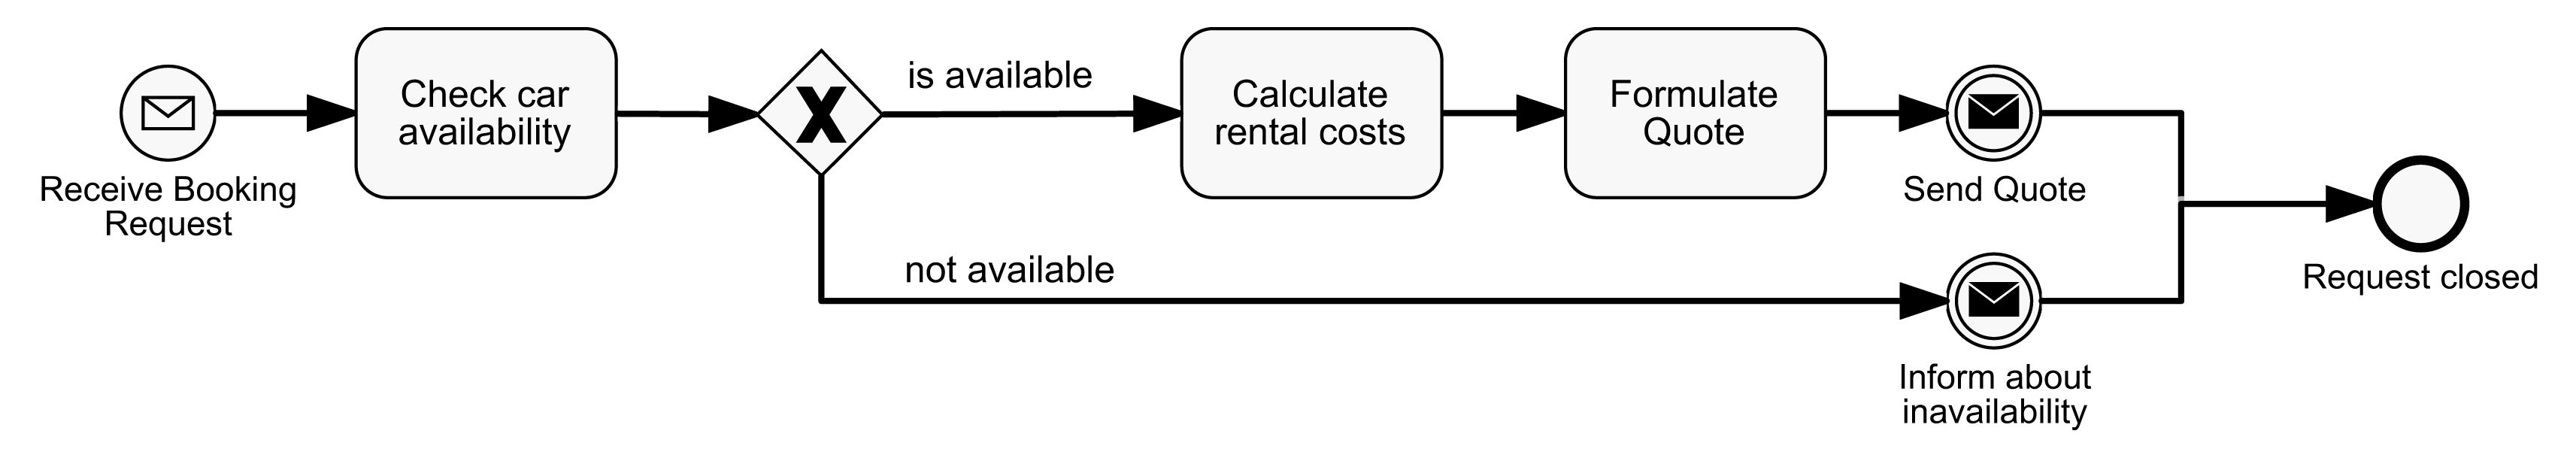
\includegraphics[width=1\linewidth]{chapters/background/intro-rental-car.png}}
	\caption{Simple BPMN model of issuing a quote for car rental}
	\label{fig:simple-bpmn-model}
\end{figure}

\autoref{fig:simple-bpmn-model} shows how a booking request might be handled in a car rental business.
Circular elements represent events, diamond-shaped elements are gateways. Activities are visualized by rectangles with rounded corners.
The given process gets instantiated whenever a booking request request is received from a customer, shown as a Message Start event. 
As a first step, the employee assigned to handle the request must check if the desired car is available. To that follows an exclusive OR-Gateway, distinguishing the further process flow depending on the availability of the car.
If the car is available, the quote must be created in two sequential tasks to be then sent out by the \textit{Send Message Event}. If the car is not available, the customer is informed about the closing of his request. 
In either case, the process ends with an \textit{End Event} after the customer was informed about the result of his request.

The example illustrates the basic use of activities, events and gateways in BPMN. However, for each type of element, activities, gateways and events, BPMN offers a variety of different kinds.
%Each of them comes in a broad variety.
The Task elements shown in the example~(\eg \,\textit{Check car availability}) are the most basic type of activities, representing \textit{a~unit of work}. The nature of a task can be further specified using task types, all activities can be additionally annotated with activity markers. Each of these modifications describes the activity semantics in a more detailed fashion.
Apart from the utilized XOR-gateway~(the execution-flow will proceed in exactly one of the outgoing branches), there is for example the parallel gateway, activating all outgoing branches. Moreover, the Event-based Gateway, which is followed only by events and continues along the branch of the first event that occurs.
Last but not least, message events are used to represent the action of sending information in the form of a message to a certain recipient. Other available event types are, for instance, timer, signal or error events. Events can occur as \textit{Start Events} (\eg \,\textit{Receive Booking Request}), where they trigger the instantiation of a process. Furthermore as intermediate events (\eg \,\textit{Send Quote}) or as end events, being fired when the process terminates. They can be \textit{catching}, \ie \,receiving a trigger, or \textit{throwing}.

Multiple participants taking part in a process can be expressed using \textit{pools}, which can be sub-divided into \textit{swimlanes}.
Interactions between different pools take place using message flows, which are depicted by a dashed arrow.
An example of such a \textit{Collaboration Diagram} is shown in \autoref{fig:bg:rental-car-customer}. It describes the previously discussed car rental process from the side of the customer, including the information exchange between rental company and customer.
When the airline issues the booking confirmation of the flight, the customer has to book a rental car and a hotel. The hotel booking is modeled using a collapsed sub-process to reduce the complexity of the model.
After issuing the rental car request, an event-based gateway shows that the process is ready to consume any one of the two event messages. If the booking was successful, the control flow proceeds to the inclusive join gateway and the process can terminate once the hotel booking is also completed. If the car rental company informs about unavailability, the customer starts looking for an alternative car option.
A data object is used to model the \textit{Request} artifact as output of the \textit{Prepare~Request} task and as input to the message throw event.

\begin{figure}[]
	\myfloatalign
	{\hspace*{-0.8cm}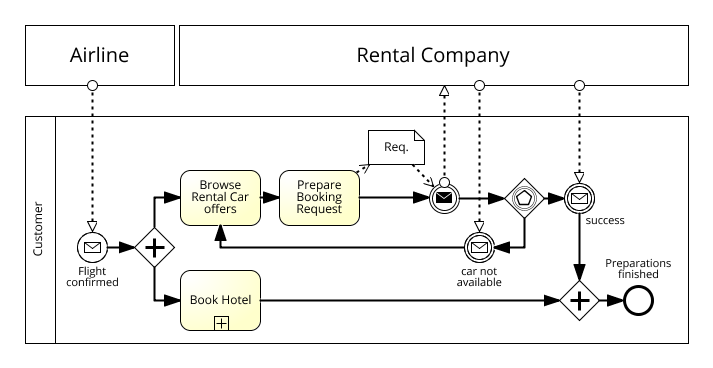
\includegraphics[width=1.1\linewidth]{chapters/background/intro-rental-car-customer.png}}
	\caption{Rental car booking process with multiple participants}
	\label{fig:bg:rental-car-customer}
\end{figure}


\section{Complex Event Processing}\label{ch:bg:cep}
The IT world is facing an exponential increase in the amount of produced data. A significant part of this data are pieces of information about real-life occurrences, such as a current sensor value, an interaction on a website or the location of a vehicle on the road.
We call this kind of strongly time-related information an \textit{Event} and the according computer science field \acf{CEP}~\cite{evtprocessing}.
More specifically, Etzion and Niblett define an event as \textit{an occurrence within a particular system or domain; it is something that has happened, or is contemplated as having happened in that domain}.
It is understood that events are of a certain \textit{event type}, defining the attributes that each event instance of the event type is composed of. An attribute is described by a unique attribute name and a data type.

\begin{description}
	\item[Definition 4 (Event):]
	An event is a tuple $e = (et, eventtime, c)$, whereas
	\begin{itemize} 
		\item
		$et$ is the event type
		\item 
		$eventtime$ is the time the event happened
		\item
		$c$ is the content of the event consisting of a set of key-value-pairs according to the content description cd of the corresponding event type $et$.
	\end{itemize}
\end{description}

%An event processing network is a collection of event processing agents, producers, consumers, and global state elements, connected by a collection of channels

Four major components take part in an event processing network: (a) An \textit{event producer} provides information to the system, (b) an \textit{event agent} processes the occurring information, so that it can be delivered to the \textit{event consumer}~(c). The components are linked through \textit{event channels}~(d).
Typically, a so-called \textit{\acs{CEP} Engine}~(also: CEP platform) is at the heart of the system, taking the role of an event agent.
Modern CEP platforms are trimmed to maximum efficiency, being able to process hundreds of thousands of events every minute.
Their main purpose is to accept incoming events from event producers, filter and match them according to selection criteria and, finally, derive a new event occurrence to be sent to the registered event consumers.

% cite luckham2008power

\paragraph{The publish/subscribe Principle}
In event-based architectures, communication takes place according to the \textit{Publish/Subscribe Principle}.
The concept essentially demands that an event processing middleware publishes events to processes only after they have issued a subscription for these events.
Consequently, there is a strict temporal order between the actions subscribe, consume and un-subscribe(\autoref{fig:bg:pubsub-workflow-temporal-order}). The consumption and un-subscription can only happen after the subscription. Once an un-subscription has been issued, no consumption can follow.~\cite{tanenbaum:2007}

% mandal also references Barros, A., Decker, G., Grosskopf, A.: Complex events in business processes. In: Business Information Systems. Springer (2007)

\begin{figure}[]
	\myfloatalign
	{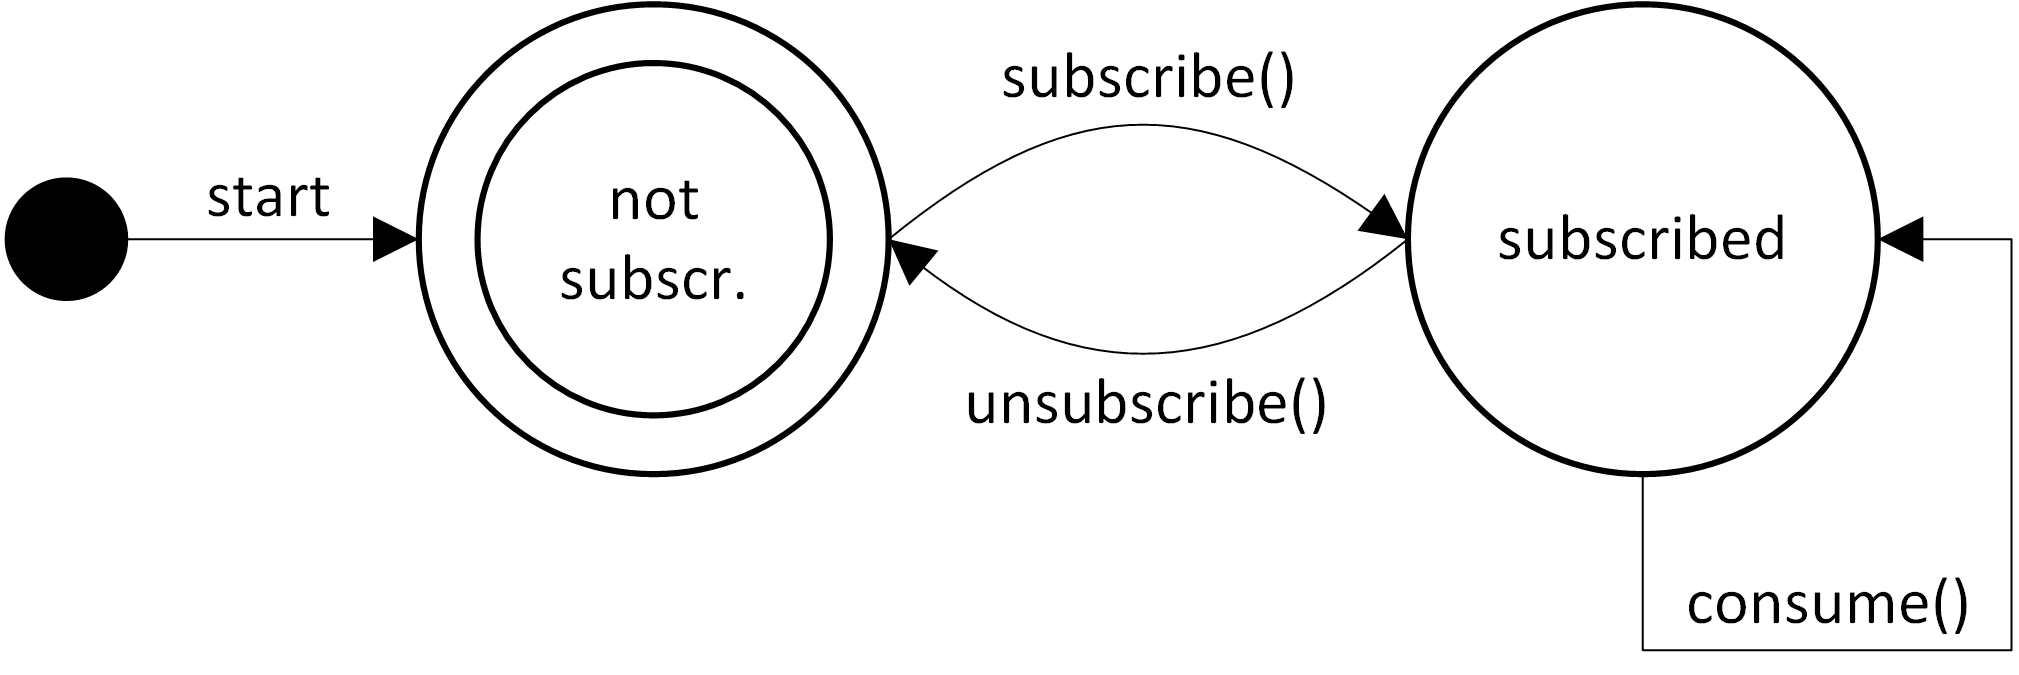
\includegraphics[width=0.6\linewidth]{chapters/background/pub-sub-statemachine.png}}
	\caption{Publish-Subscribe workflow expressed in a state diagram}
	\label{fig:bg:pubsub-workflow-temporal-order}
\end{figure}


One of the main advantages of this principle is, that the involved parties are \textit{referentially decoupled}. They do not need to explicitly refer to each other, an aspect that is also acknowledged in~\cite{evtprocessing}.
Their decoupled nature facilitates the management and development of event processing networks. Event producers and consumers might change frequently.
Whenever a new event source is available it can be connected to the CEP platform without considering all future consumers. Consumers can subscribe and un-subscribe without influencing the operations on the consumer side.


\paragraph{Stream Processing}
To be able to cope with potentially large amounts of data, Complex Event Processing Platforms work on the basis of \textit{stream processing}.
In a traditional relational database, information is stored for an indefinite amount of time. When a user queries the data store, the system processes the tabular data and calculates the requested result. 
The advantage of this approach is that the user can access historic data at any time, as long as it is not explicitly deleted from the database.
In many occasions, the amount of available data significantly surpasses the storage capacities and that concept can no longer be followed.

Stream processing addresses the mentioned challenge by largely reducing the amount of data that is persisted in the system. Instead, it is the goal to keep only those pieces of information, that are necessary to process a result for currently registered queries.
Incoming data objects, or events in the case of a CEP platform, enter the event stream and are immediately evaluated against all existing query expressions. If the information is not required to process any of the queries, it is deleted instantly. If an event matches a query, a notification is sent to the subscribed consumers. \autoref{fig:bg:stream-processing} illustrates the concept.
As a consequence, a certain event can not be part of a query result, if that query has been registered after the occurrence of the event.
In case aggregated information is demanded by the query, the stream processor will internally store aggregated information, but not keep every information that led to the aggregated value.~\cite{streamprocessing} 

\begin{figure}[]
	\myfloatalign
	{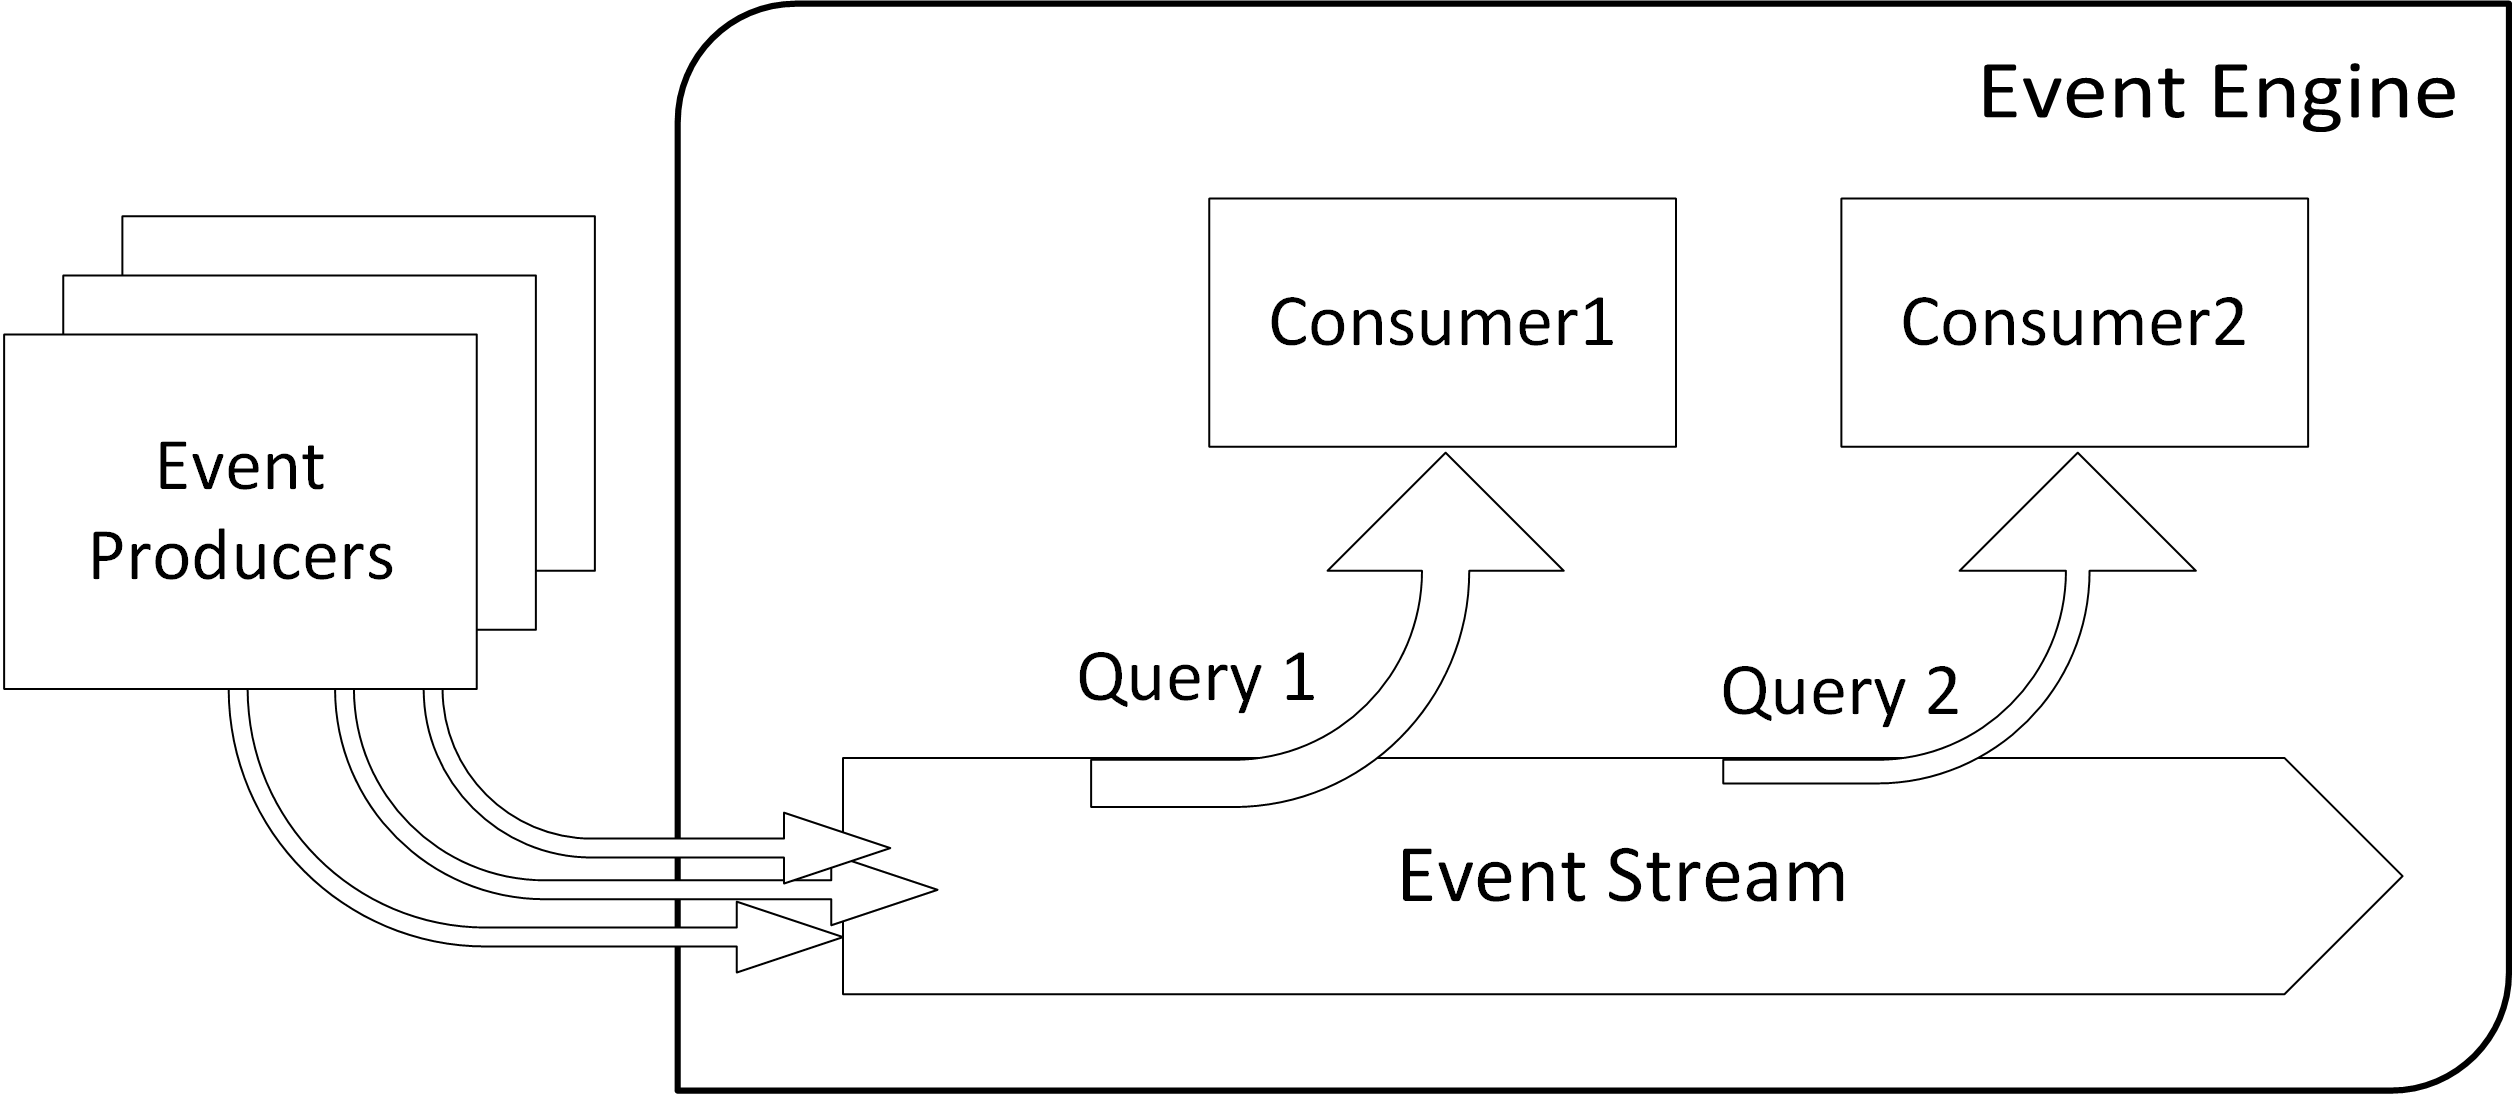
\includegraphics[width=0.7\linewidth]{chapters/background/cep-stream-processing.png}}
	\caption{Stream processing concept applied in a CEP Engine}
	\label{fig:bg:stream-processing}
\end{figure}

The subscription to an event in a CEP platform is primarily defined by an \textit{Event Query}.
Many modern event query languages are inspired by \acs{SQL}, but cannot be entirely compliant due to the different underlying data processing concept.
When formulating event queries, it is essential to consider the stream processing principle.
For the illustration of the concepts, this thesis relies on the Esper \ac{EPL}~\cite{esperhome}, utilized in Esper-based event processing engines like the one employed in the presented reference implementation, \autoref{ch:implementation}.
A simple event query in Esper looks as follows:

\begin{lstlisting}[language=sql,caption={Sample Query in Esper EPL},label=lst:epl-query-example]
	SELECT occurrencetime, delay, delayreason 
	FROM eurotunnel.win:time(2 hour)
	WHERE delay > 30
\end{lstlisting}

\section{Event-driven Business Process Control}
The disciplines of Complex Event Processing and Business Process Management are connected in \acf{EdBPM}, which discusses the uses of events to enhance business processes~\cite{evtprocessing}.
There are two usage scenarios for events in BPM. In Business Activity Monitoring and analysis, events are published by the process engine and processed to obtain analytical information, for instance about process status, efficiency or errors.
This thesis considers events from the second perspective, \acf{EdBPC}. The field focuses on the business process as an event consumer.
Within business processes, event-based communication can for example be used to exchange information between participants or to react to external events. While the BPMN supports a large variety of different events, we are going to investigate message events specifically. Whenever talking of an event-occurrence, it can be assumed that the term \textit{event} implicitly refers to a message-event in the BPMN context.

\ac{EdBPC} using external event sources is facilitated by connecting the business process engine to an event engine.
As explained in \autoref{ch:bg:cep}, interactions with a CEP platform follow the publish-subscribe paradigm.
In the BPM scenario, this means that a subscription to events must be present, so that events can be received by the process engine and correlated to a specific message element within a process instance~\cite{Baumgrass2016}.
The correlation has to be performed by the process engine on the basis of context information, for example a subscription identifier incorporated inside every CEP message. 
An interaction between process engine and event engine is illustrated in \autoref{fig:bg:subscription-workflow}~\cite[,\,p.\,13]{mandal:2017} at the example of the event engine Unicorn.
Note that a different event engine might implement the work-flow slightly differently, but still follow the same general concept.
In the given case, the process engine first issues a \acs{HTTP} POST call containing the subscription query a notification-path. The path contains the address of the desired notification recipient in case a matching event occurs.
The event engine answers that call with a unique identifier associated to that single subscription.
As soon as an event occurs that matches the query, the event engine sends the query output along with the subscription identifier to the process engine which can correlate the event back to the associated instance.
In the next chapter, we will discuss when exactly the event subscription is issued by the process engine.

\begin{figure}[]
	\myfloatalign
	{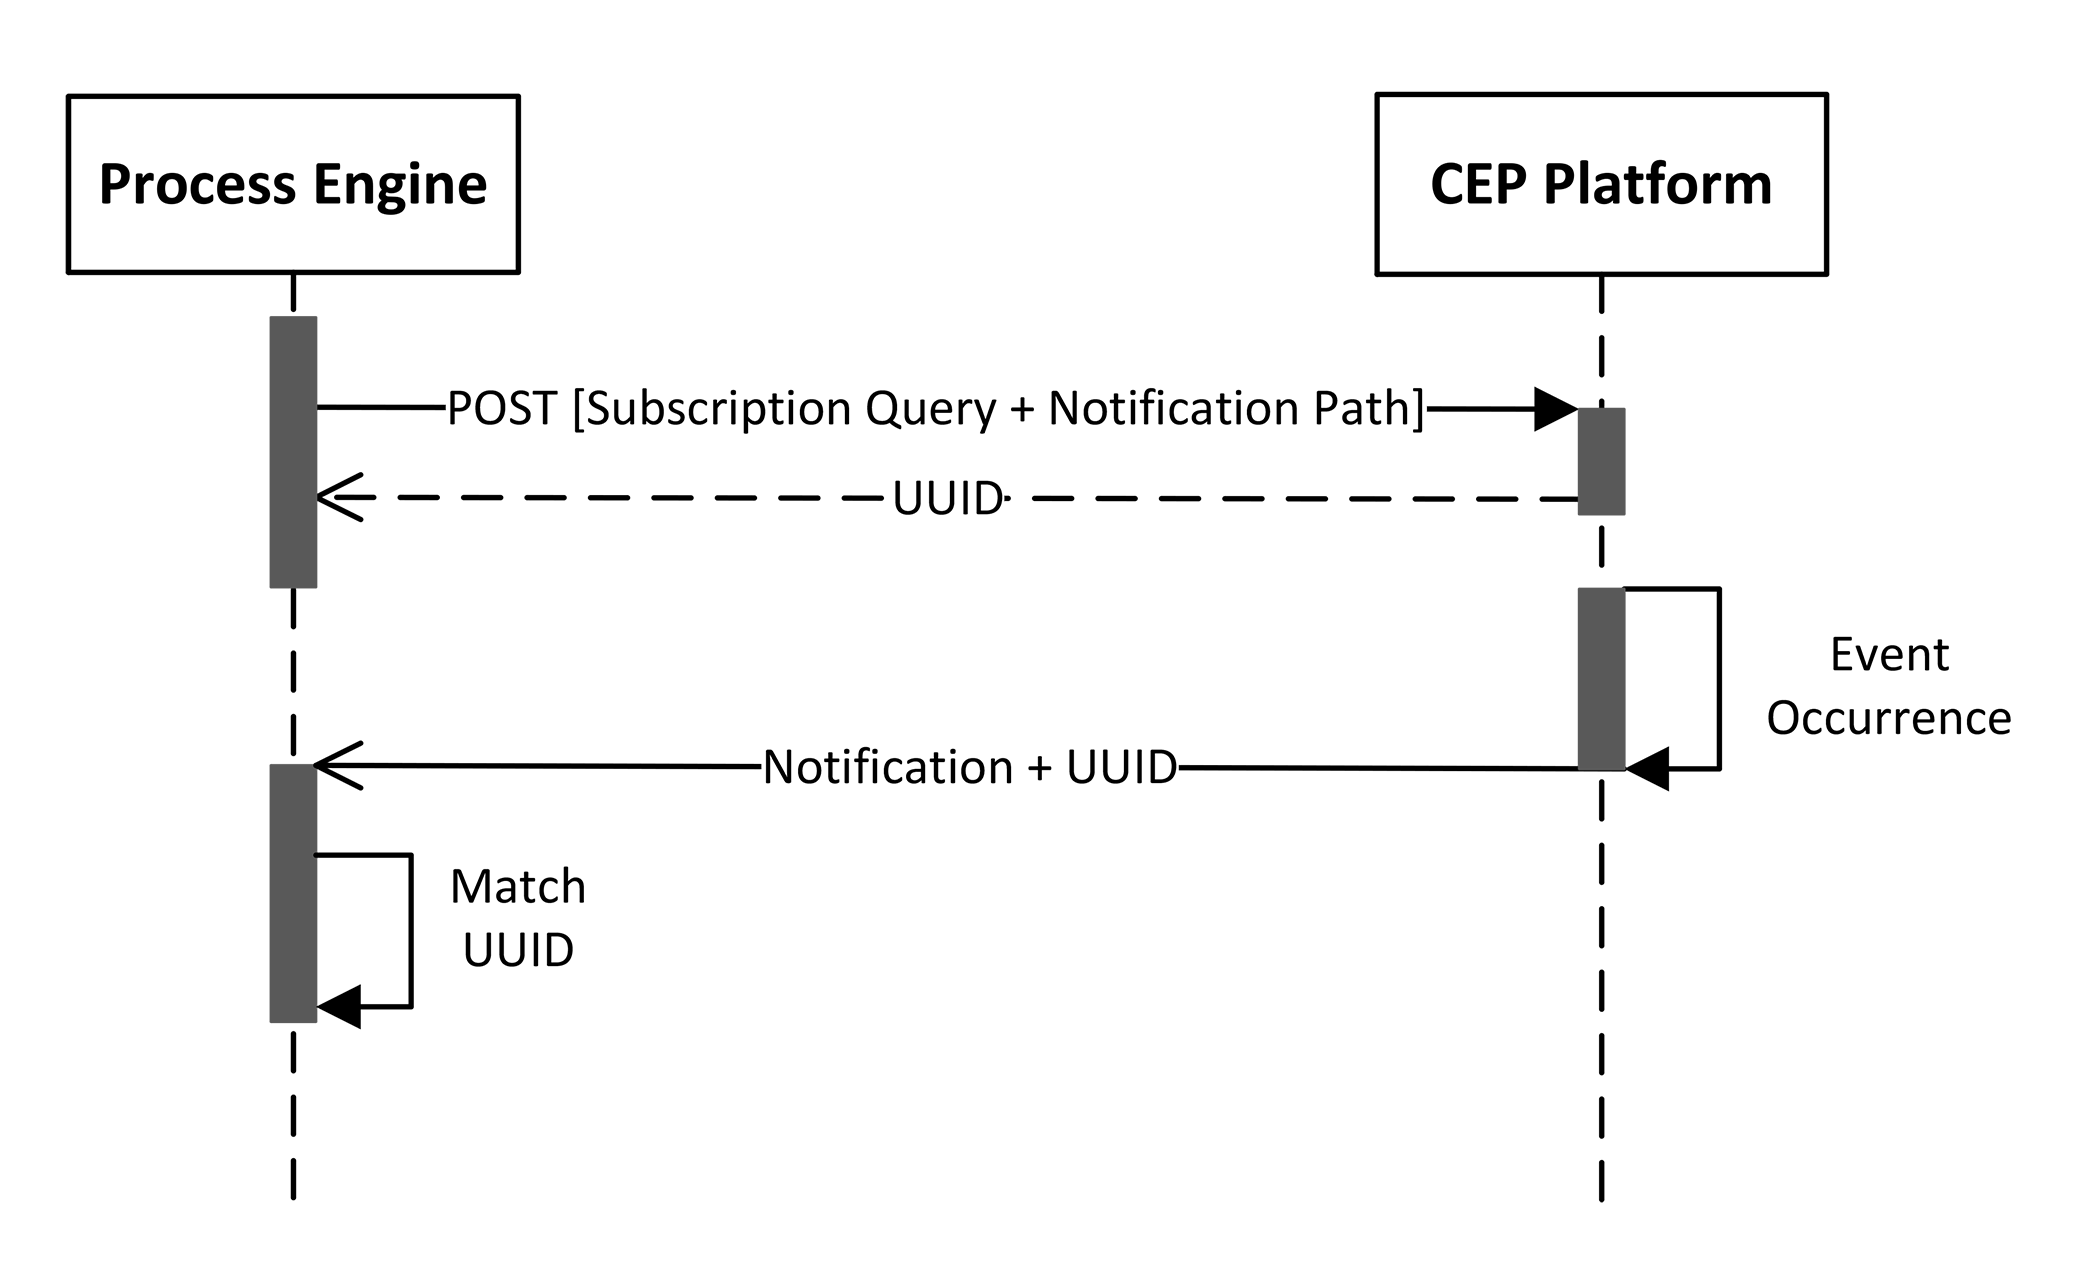
\includegraphics[width=0.6\linewidth]{chapters/background/subscription-workflow.png}}
	\caption{Even-subscription work-flow between process engine and event engine.}
	\label{fig:bg:subscription-workflow}
\end{figure}

%- no standard yet available to do subscription in bpmn
%- it must be assumed that the subscription is either already active or explicitly modeled in BPMN, e.g. using a service task
%- OR given the BPMN spec it is generally assumed that the subscription is executed as soon as en event is enabled
%- further analysis of this topic is provided in ...
%- the time of event subscription is clear for start events
%- Correlating events to process instances






\cleardoublepage%************************************************
\chapter{Problem Statement}\label{ch:problemstatement}
%************************************************

Event subscription is an essential part of event-driven architectures and must consequently be considered when using events in business processes.
While the use of external events is an active topic in research, most approaches only briefly discuss the subscription mechanism and use the \acs{BPMN}~semantics for orientation~(\eg \,\cite{Pufahl2017} and \cite{Baumgrass2016}).
Though event subscription is not directly addressed in the BPMN~specification, the descriptions on intermediate events state:

\medskip
\textit{"For Intermediate Events, the handling consists of waiting for the Event to occur. Waiting starts when the
Intermediate Event is reached. Once the Event occurs, it is consumed."}~\cite{bpmnspec},~p.~440

\medskip \noindent The usual interpretation of this excerpt is that the subscription to the event takes place as soon as the event gets enabled, the un-subscription when the event terminates.
As pointed out by Mandal~et.~al.~\cite{mandal:2017}, these subscription semantics significantly limit the flexibility of using events in business processes and can cause undesired behavior and fault.
Due to the strict temporal order between event subscription, occurrence and un-subscription as required by the publish-subscribe paradigm, any events that occur before the enabling of the event element will be ignored by the process execution.
That reduces the timespan for events to occur to a potentially small part of the total execution time and means that crucial events might be missed which can delay or block a process execution unnecessarily.

In the following section, the problem is further illustrated at the example of two motivating scenarios.
The observed situations then lead to the definition of \textit{Event Occurrence Scenarios} and the derivation of a set of requirements that must be fulfilled by a mechanism for flexible event subscription in business processes.

\section{Motivating Examples}\label{ch:motivatingexamples}
% some has been mentioned in the introduction
%illustrate the complexity

To allow a better understanding of the issue, event-driven use-cases from two different domains are presented in the following.
The cases are revealed through their standard BPMN representation.
It is illustrated, why the time of event subscription is of great importance which motivates to study the mechanics and implications of event subscription in business processes.

\paragraph{Delay of a logistics process}
The first example~(\autoref{fig:example-eurotunnel}) is taken from the logistics domain and shows a truck transport that has to cross the English Channel.
The truck driver receives the transport plan for his next tour from France to the UK. By default, the company crosses the Channel using the Eurotunnel, an underground train connection between London and Paris.

\begin{figure}[]
	\myfloatalign
	{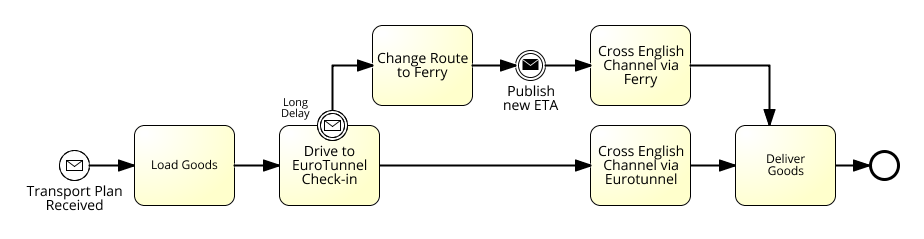
\includegraphics[width=1\linewidth]{chapters/requirements/Eurotunnel-simplified.png}}
	\caption{BPMN Model of a Logistics Process using events for route~optimization~(Example 1.1)}
	\label{fig:example-eurotunnel}
\end{figure}

After loading the goods at the factory, the truck will head towards the check-in location of the Eurotunnel.
If everything runs on schedule, the truck crosses the channel on the train and then delivers the goods in Great Britain.
Alternatively, the process considers a route using the ferry from Calais~(FR) to Dover~(UK).
The Eurotunnel administration publishes delay information approximately every 30~minutes through an RSS feed on their website. While it mostly operates on schedule, delays ranging from 15~minutes to several hours occur regularly. It can happen that new information is not published for multiple hours.
Significant delay events (delay~>~30~minutes) are received through a boundary catching message event attached to the activity \textit{Drive to Eurotunnel Check-In}. The boundary event is interrupting, hence the activity is canceled if a delay occurs.
The transport continues towards the ferry terminal and crosses the English Channel over sea. After crossing the channel, the goods are delivered to the recipient.

As interpreted from the BPMN specification, the subscription to the boundary event is issued as soon as the related activity is enabled.
Given that events arrive every 30~minutes, there can be a gap of up to half an hour, before the first information becomes available.
In the worst cases, when data isn't published for several hours, this gap will be even bigger.
Let's consider a very busy weekday; A technical fault occurred in the tunnel earlier that day and the train runs 3 hours behind schedule.
The last information on the RSS feed was published at 2:35\,pm. At that time the truck driver is still in the process of loading goods, finishing the activity at 2:40\,pm.
Following the process definition, the driver now departs towards the Eurotunnel check-in.
The system publishes updated information at 3:15~pm, operations are still 2:30\,h behind schedule. The message gets received through the process and the truck driver takes the alternative route to the ferry, but only after heading to the Eurotunnel for 35~minutes. The late change of plans causes an unnecessary delay to the shipment.

\begin{figure}[]
	\myfloatalign
	{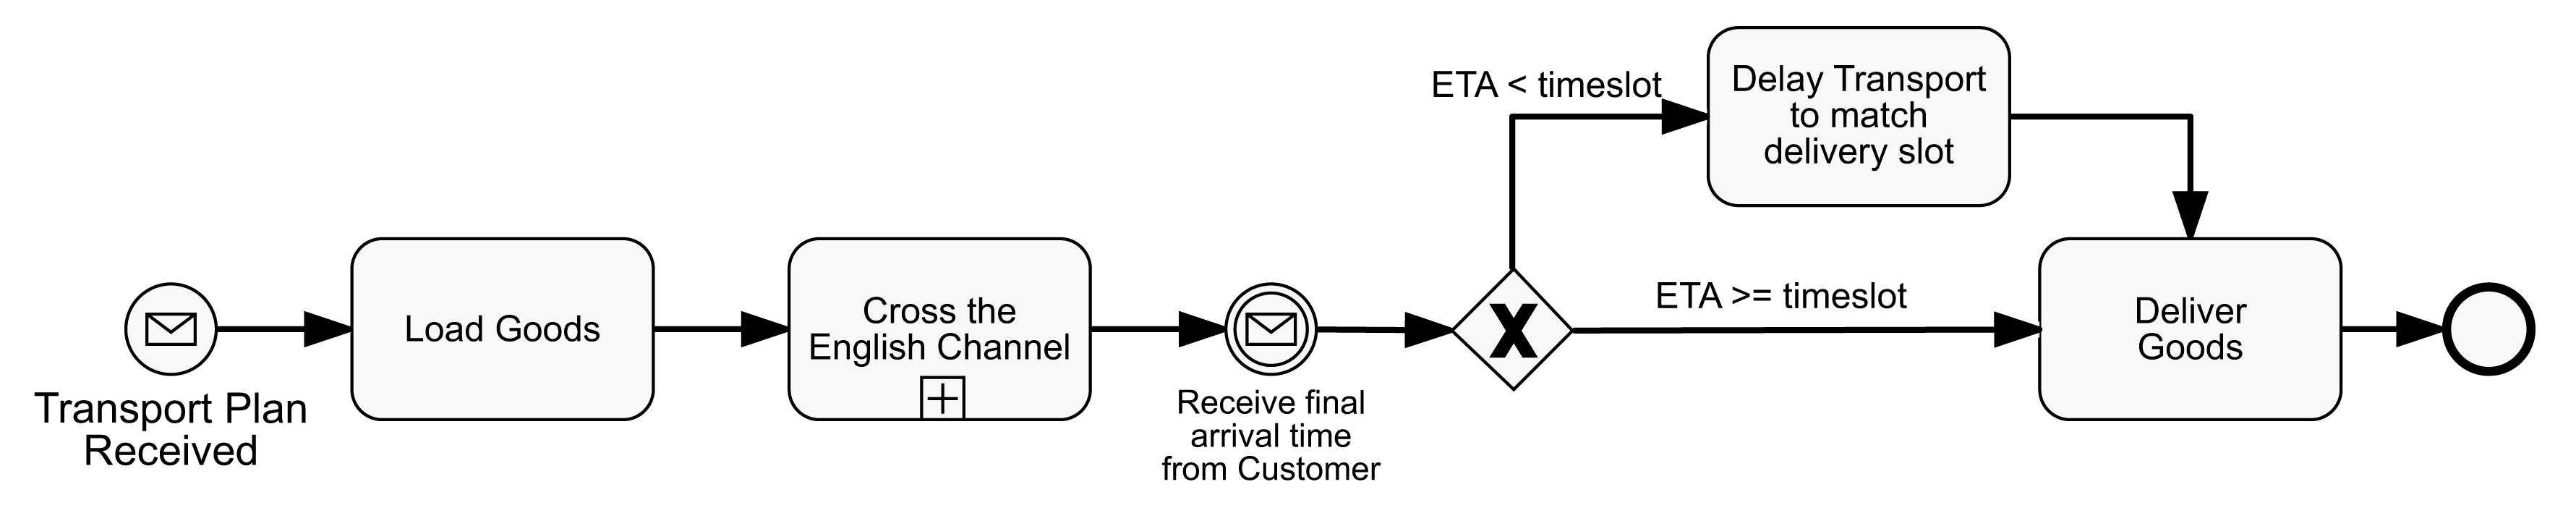
\includegraphics[width=1\linewidth]{chapters/requirements/Eurotunnel_part2.png}}
	\caption{Transport via English Channel that is timed to a delivery~slot~(Example~1.2)}
	\label{fig:example-eurotunnel-part2}
\end{figure}

\autoref{fig:example-eurotunnel-part2} is an extension of the the transport process.
In logistics, it is common that a delivery cannot be accepted at an arbitrary time. Instead, the receiving party assigns delivery windows to the transport company.
The transport must arrive during the given time window, otherwise the delivery cannot be completed.
After crossing the English Channel, the process model shows the catching of a message event containing the desired final arrival time at the factory. There is an agreement with the factory, that the delivery slots will be approved 2~hours before the expected arrival.
If the current ETA of the transport is greater or equal to the arrival time, the driver will head to the drop-off point immediately. If the transport is ahead of schedule, the driver will have to delay the delivery to match the time window.

The presented process model illustrates another complexity of using events in processes. Again, the listening to the announcement of a delivery window will start when the event element is enabled, in this case after crossing the English Channel. 
Until an event has been received, the process will not continue. 
Much worse: if the receiving party sends out the arrival time information too early, \ie~while the truck is crossing the channel, the event is missed. If it is not issued again, the process cannot receive a message and will get stuck indefinitely waiting to catch the event.

Neither of the two presented catch events allow for an efficient and reliable execution of the process. They can cause unnecessary delays and even blocking of the process execution.


\paragraph{Up-to-date shipping information for an order}
\begin{figure}[]
	\myfloatalign
	{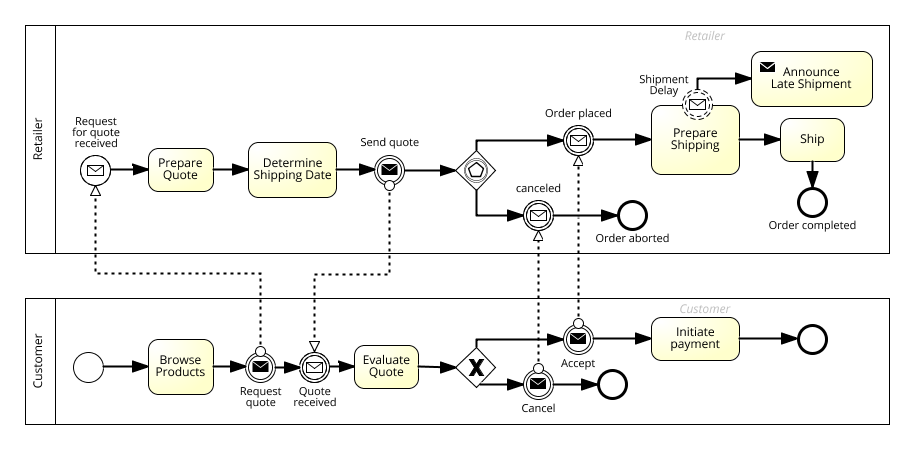
\includegraphics[width=1\linewidth]{chapters/requirements/Retail-Order.png}}
	\caption{Model of a retail order management process (Example 2)}
	\label{fig:example-order}
\end{figure}

A~similar situation can be observed in the order-management process depicted in \autoref{fig:example-order}.
It describes the interaction between customer and seller in a traditional distance retail scenario: After browsing the product catalog, the customer requests a quote for the articles he or she is willing to buy.
The retailer makes an offer including an approximation of the expected shipment date and sends it to the customer. That quote is then either accepted or not and the payment is issued if necessary.
Once the retailer is informed about the placement of the order, the products are packed and shipped as soon as possible.
For articles that are not currently in stock, the retailer must await the shipment from the factory. If any of the factory-shipments is delayed, the retailer cannot ship in time and will announce a delayed shipment date to the customer.
This situation is modeled through a non-interrupting boundary event attached to the \textit{Prepare Shipping} activity, which triggers the sending of the updated shipment date to the customer.

The process shows a number of similarities, but also differences in terms of event-use when compared to the logistics process in Example~1.
At first we look at the three intermediate catch events, \textit{Quote~received}, \textit{Order~canceled} and \textit{Order~placed}.
In each of the cases, the event to be caught is the direct response to a message that was sent right before. While the process will also enter a waiting state until the response arrives, that waiting is not to be interpreted as an unnecessary delay to the process execution.
Other than in Example~1.2\,(\autoref{fig:example-eurotunnel-part2}), there is nothing useful to do before the response is received.
It is furthermore worth noting that the response messages cannot be missed, because the message catch event immediately follows the message send event.

A different situation holds for the boundary event \textit{Shipment Delay}.
While the subscription to a Eurotunnel event can be issued at any time, it does not depend on any process data, the shipment delay has to be observed for each product that is part of the order. A subscription can therefor not be executed before the activity \textit{Prepare~Quote} has terminated.
The Esper query to obtain delay information about the product with the id 123 looks as follows:

\begin{lstlisting}[language=sql,caption={Esper EPL Query to obtain delay information for a product},label=lst:epl-query-shipping-delay]
SELECT newArrivalDate, delayAmount, delayReason, productId
FROM shippingdelay
WHERE productId = 123
\end{lstlisting}

\noindent Conforming to the definition of the process, the system will listen to shipment delays once the activity \textit{Prepare~Shipping} is enabled and therefor much later than possible.
Any events that occur after the completion of \textit{Prepare~Quote} but before \textit{Prepare~Shipping}, cannot be considered in the process execution and the customer will not be informed about a possible late shipment. That will, for instance, concern events that occur while the customer makes the decision about accepting or canceling the order.

% The first of these three follows the \textit{Send/Receive} Service Interaction Pattern. \todo[inline]{missingref}
% Two parties interact 

\medskip \noindent 
The two presented examples have illustrated the complexity of using events in business processes, especially when all possible event occurrence times are taken into consideration.
Differences have been pointed out as to how exactly the event is placed in the process, if it waits for a direct response to an earlier request or if the event occurrence is unrelated to the execution of that very process.
Motivated by this complexity and the possible implications, it is the goal of this work to evaluate the capabilities of BPMN and to present a concept for the flexible handling of event subscription in business processes.


\section{Event Occurrence Scenarios and Time of Subscription}\label{ch:ps:eos}
Given the motivating examples, a generic set of \textit{Event Occurrence Scenarios} is defined in this section. 
Each of the scenarios represents a real-world situation and process implementations need to be capable of handling them to avoid negative effects.

\medskip \noindent
The dominant variable to consider is the event occurrence time.
According to the BPMN specification, it is possible to catch an event if it occurs after the event element is enabled. As shown before, it is often impossible to control occurrence time and events do occur outside of the listening time intervals.
An \ac{EOS} describes the time of event occurrence in relation to a specific step in process or engine execution.
The life-cycle of a process within a process engine is explained in \autoref{ch:bg:bpm} and taken as reference. It is assumed that the process and event engine are configured and running.
An event is considered to always occur before or after a life-cycle step or in between two consecutive steps. 
Given the life cycle steps \textit{process deployment}, \textit{process instantiation} and \textit{event enabling}, the following occurrence scenarios are distinguished in this work:
% they have an implicit temporal order

\begin{aenumerate}
	\item[$EOS_{1}$] While the BPMN event element is enabled
	\item[$EOS_{2}$] The event does not occur
	\item[$EOS_{3}$] Between process instantiation and \\the enabling of the BPMN event
	\item[$EOS_{4}$] Between process deployment and \\process instantiation
	\item[$EOS_{5}$] Before process deployment
\end{aenumerate}\label{def:occurrence-times}
% they are ordered this way to be in line with the assessment chapter

\begin{figure}[]
	\myfloatalign
	{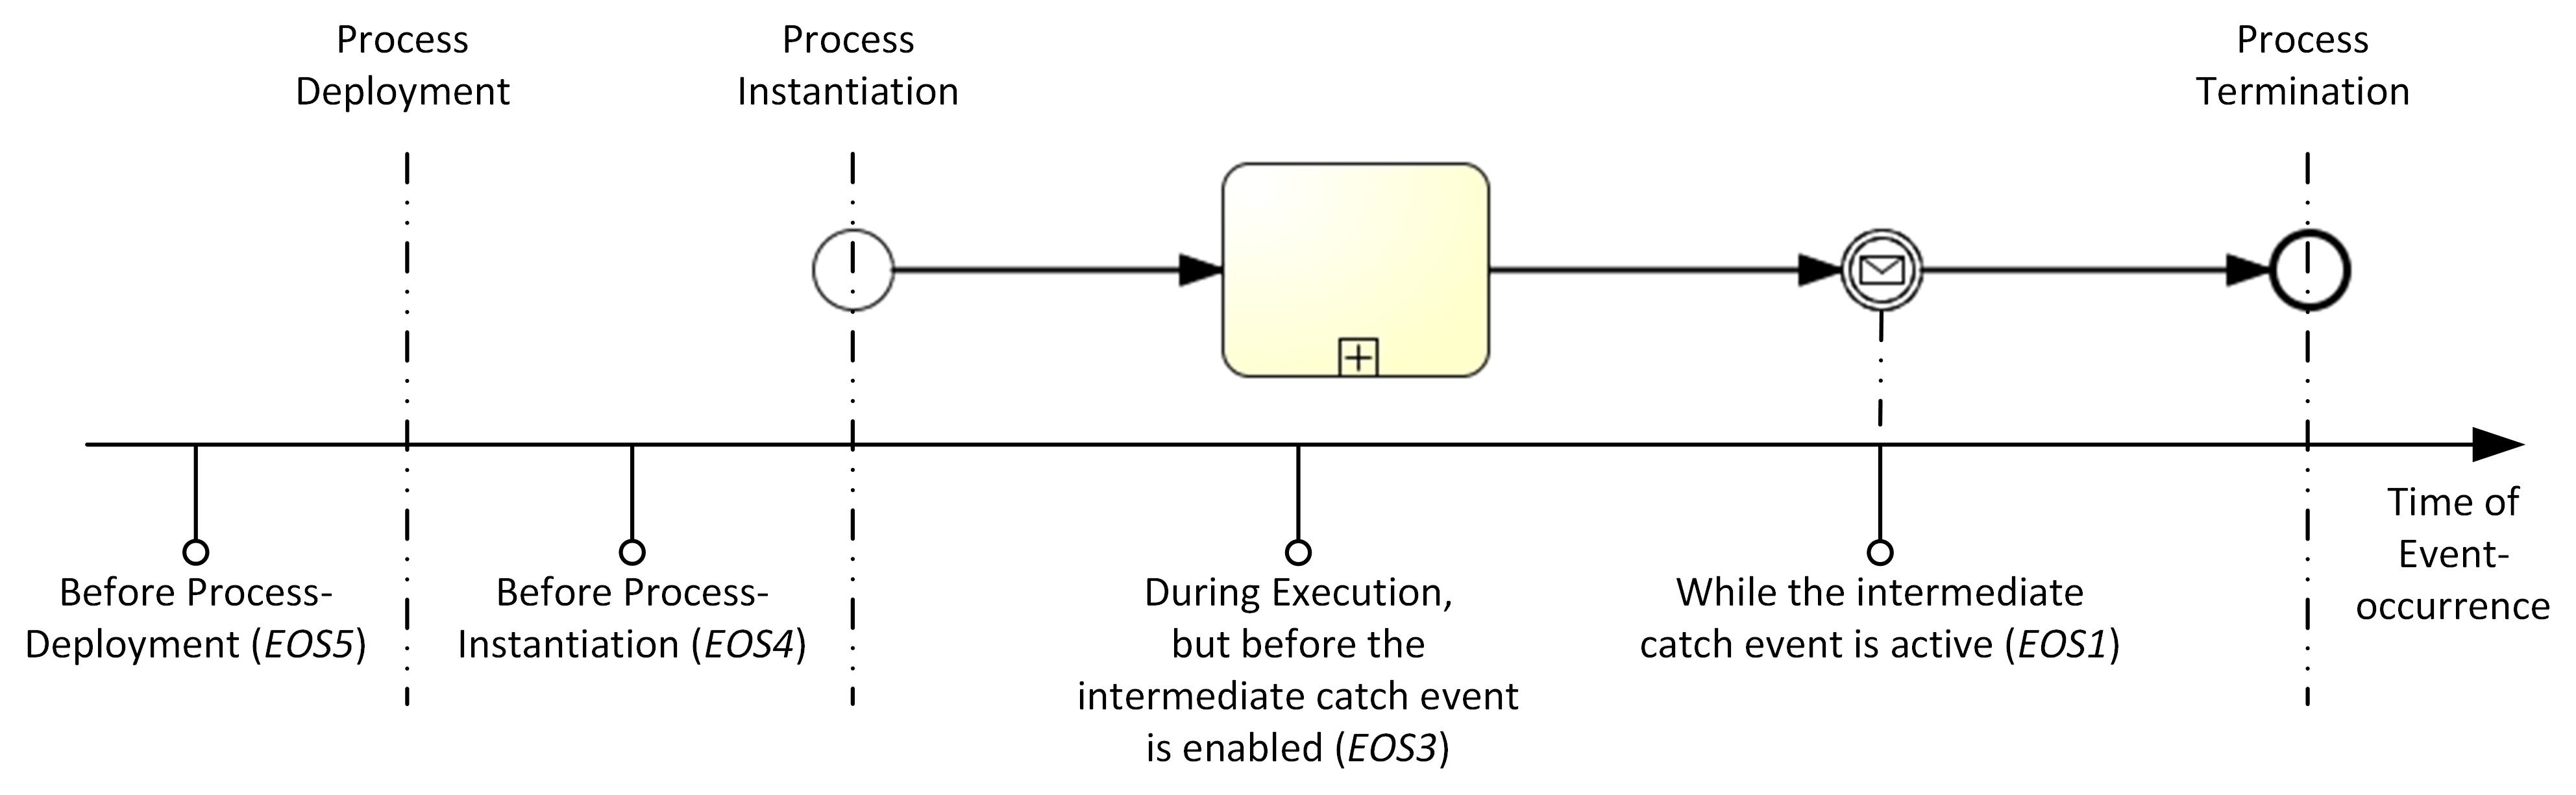
\includegraphics[width=1\linewidth]{chapters/requirements/timeline_event-occurrence.png}}
	\caption{Event Occurrence Scenarios}{Possible times of event occurrence in relation to a process execution life-cycle. \textit{EOS2} (event does not occur) not illustrated.}
	\label{fig:occurrence-timeline}
\end{figure}

\noindent An overview of the EOSs and the related life-cycle steps is provided in \autoref{fig:occurrence-timeline}, which uses a time-line to illustrate the possible event occurrence times.
The model deliberately excludes event occurrences after termination of the event element, because that would presume that there is no more interest in the event as the execution flow continued on another branch. Otherwise, the process will remain in waiting state until the event occurs.

As introduced in \autoref{ch:bg:cep}, there is a strict temporal order between event subscription, consumption and un-subscription.
To catch an event that occurs as described in any of the EOSs, the related subscription operation has to be executed before the start of the time interval associated with the EOS.
On that basis, the latest possible event subscription time can be derived from each event occurrence scenario and is as follows:
\textit{before process deployment}~($EOS_{5}$), \textit{during process deployment}~($EOS_{4}$), \textit{at process instantiation}~($EOS_{3}$) and when the \textit{BPMN event element is enabled}~($EOS_{1}$).

It is important to highlight that the subscription to an event source can depend on additional context information or process data, which can be a significant limitation to the possible subscription time.
That situation is illustrated in \textit{Example~2}~(\autoref{fig:example-order}), where the subscription to the shipment delay information cannot be executed before the \textit{Prepare~Quote} activity is completed.
More generally put, a \textit{subscription~dependency} is defined as follows:

\begin{description}
	\item[Subscription Dependency]
	The subscription operation is \textit{dependent}, if any of its parameters, for instance the event query, contains a variable value that has to be determined at the time of subscription.
	The value might reference a piece of information from the process instance context, an engine-wide piece of data or external information.
	In case of a dependence, the subscription cannot be issued before the associated information is available.
\end{description}

If a subscription dependency resolves before the process execution reaches the event element, it should still be possible to flexibly chose the subscription time in the process.
For that reason, in addition to the four subscription-time options presented earlier, an additional option \textit{at any time during process execution} must be available.


\section{Requirements Definition}\label{ch:requirements}
The previous sections have exemplified how the BPMN execution semantics and notation capabilities limit users when using events in business processes. 
Now, these deficiencies are formalized into an initial set of requirements additional to the features offered by BPMN.
They build the foundation for enhancing BPM solutions towards flexible event subscription management~(\autoref{ch:flexibleeventsubscription}).
Before that, the formal requirements will be used to evaluate the capabilities of current Process Management Solutions~(\autoref{ch:assessment}), which results in an additional set of shortcomings \textit{S1} to \textit{S3} of current solutions presented in \autoref{ch:ass:discussion}.

%\medskip \noindent
%It shall be noted that the requirements \textit{R2.2} and \textit{R3} introduced in this chapter have also been pointed out by Mandal~et.\,al. in their work on early subscription and event buffering\,\cite{mandal:2017}.
%Note that the need for flexible event subscription has also been pointed out by Mandal~et.\,al. in their work on early subscription and event buffering\,\cite{mandal:2017}. The authors follow a similar line of argumentation and also specify the requirement for a flexible time of subscription and event buffering.


\paragraph{R1: Subscription Fundamentals}

\begin{description}
	\item[R1.1 Subscription to an Event Source:]
	To enable the reception of events from a publish/subscribe event source, the subscription operation must be part of the execution flow. 
	In accordance with the obligatory temporal order of operations, the subscribe operation must happen before an event can be received and/or the un-subscription takes place.
	\item[R1.2 Un-subscription:]
	As soon as events from the source must not be received anymore, an un-subscription has to take place.
	\item[R1.3 Availability of Information:]
	For each event that is used in a business process, all information necessary to execute an event subscription in the given execution environment must be available.
	That information generally includes the event query, the address of an event processing platform and auxiliary information to establish the communication, for instance authentication data.
	%While the event query is associated to a specific event element and must therefor be part of the process model, the process platform information might be valid for potentially all processes and can be made available through a global data store.
	\item[R1.4 Variables in Event Queries] 
	To adapt an event subscription to execution- or time-specific information, variables can be utilized as part of the query string.
	At the time of event subscription, these variables must be replaced their current values before the subscription is executed.
	
\end{description}

\paragraph{R2: Event Subscription Time}

\begin{description}
	\item[R2.1 Explicitness:] 
	For each event that is used in a business process, it must be possible to derive the time of event subscription from the process model. The time of subscription may either be explicitly stated or defined implicitly.
	\item[R2.2 Flexibility:] 
	The time of subscription can be influenced independently from the place the event element takes in the model. Timing options are made available to catch events according to any of the event occurrence scenarios EOS1, EOS3, EOS4 and EOS5. 
	Consequently, the options must include but are not limited to the subscription before process deployment, during  pr. deployment, at process instantiation, subscription at an arbitrary but explicit time during process execution or when the event element is enabled.
	Thereby, also events that occur after the time of subscription, but before the event element is enabled shall be available to be consumed.~(cf.\,\cite{mandal:2017})
	%By that means, the variability of the time of event occurrence can be specifically addressed in the process model and unnecessary delay or blocking of the execution can be reduced.
	\item[R2.3 Awareness of Subscription Dependencies:]
	The additional flexibility provided through \textit{R2.2} is limited by the use of variables in event queries~(\textit{R1.3}) and the implicit dependencies on context information.
	The execution environment must only allow a subscription time after the resolving of all dependencies.
	
	Dependencies can exist within a certain process instance, for example when an information from a local DataObject is referenced in a query. In more complex scenarios, the subscription might depend on data from other process instances or even other processes which must first be obtained.
\end{description}


\paragraph{R3: Event Buffering}

\begin{description}
	\item[R3.1 Buffering Principle:]
	%To make all events since the subscription time available during process execution, matching events need to be stored temporarily.
	As introduced by \textit{R2.2}, an indefinite time can pass between the time of subscription and the consumption of the event.
	While the subscription operation generally assures that the event is received, it is necessary to temporarily store it until the consuming element is reached.
	
	This temporary storage is referred to as an \textit{Event~Buffer}.
	The storage must be designed to fulfill the semantics demanded by \textit{R2.2} which means that any event that occurs after the time of event subscription must be available to consume.
	
	\item[R3.2 Buffer Scope:]
	The flexible event subscription time~(\textit{R2.2}) allows an event subscription after process instantiation, but also before process instantiation or deployment.
	It can be inferred that an event buffer operates either in the scope of a process instance, a process definition, or in the scope of the complete execution environment.
	To implement all event subscription times stated in \textit{R2.2}, the execution environment must support event buffering in each of the three scopes. 
	The provided concept must make clear to the user, which scope is referenced at any point in time.
	
	\item[R3.3 Buffer Policies:]
	The behavior of a buffer in any occurring situation must be specific.
	The parameters necessary to specify the behavior are referred to as \textit{Buffer Policies}, following the notion chosen by  Mandal~et.\,al.\,\cite{mandal:2017}.
	
	\item[R3.3.1 Lifespan Policy:]
	Given that the time between the event subscription and its consumption may be indefinitely long, process designs can require to limit the maximum time an event is held in the buffer.
	%A parameter must be offered to specify this timespan.
	
	\item[R3.3.2 Consumption Policy:]
	Requirement \textit{R3.2} implies that buffers can be shared among process instances of the same process and other processes.
	In this scenario, it needs to be defined if an information is consumed from the buffer upon retrieval, or if the information remains in the buffer for other participants to access. 
		
	\item[R3.3.3 Size Policy:]
	Provided that multiple events can occur between the time of subscription and the enabling of the event element, it must be specified for each buffer, how many events should be stored for later consumption.
	%In basic scenarios, where a buffer is only accessed a single time by one catch event in one process instance, a fixed buffer size of one element will be sufficient. However, if a buffer is accessed multiple times or shared among instances, the buffer size may vary between~1~and infinity.
	
	\item[R3.3.4 Retrieval Order Policy:]
	If multiple events are stored in the buffer~(\textit{R3.3.3}), it must be defined, in which order the events are provided for consumption. 
	%The order can be chosen as \textit{First in first out}~(FIFO) or \textit{Last in first out}~(LIFO) 
	
\end{description}




\cleardoublepage%************************************************
\chapter{Assessment of current Business Process Management Solutions}\label{ch:assessment}
%************************************************

The lack of flexibility in handling event subscription in business processes has been outlined in the previous chapters and a set of extended requirements to process management solutions have been presented.
In this section I take a closer look at the capabilities of current solutions with regards to the event occurrence scenarios to get a better understanding of the issues that arise when working with event subscription in business processes.
The assessment will be carried out using BPMN and Camunda, a state-of-the art and widely adopted business process engine.
The main goal is to identify and illustrate the shortcomings of the current process technology stack. These shortcomings will be referenced in addition to the presented requirements to develop a more refined subscription handling model in the following chapter. \todo[inline]{"subscription handling model"?}

\todo[inline]{which functionality should be evaluated exactly?: all occurrence scenarios, but no buffer policies. The buffer will always store the last version of the event and also deliver that version.}

\section{BPMN Models in presence of the Event Occurrence Scenarios}
Chapter X has revealed that processes can run into deadlocks if events do not occur at the right time \todo[inline]{.}
\begin{figure}[]
	\myfloatalign
	{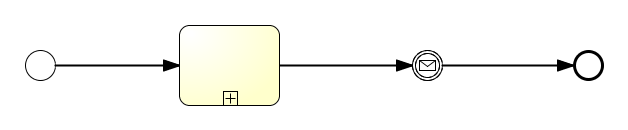
\includegraphics[width=1\linewidth]{chapters/assessment/process-with-intermediate-event.png}}
	\caption{Abstract Process using an Intermediate Catch Event}\label{fig:abstract-process-with-event}
\end{figure}

\autoref{fig:abstract-process-with-event} shows a generalized process that uses an Intermediate Catch Event just before process termination.
In this section I first describe for each Event Occurrence Scenario how this simple event implementation behaves in presence of the given scenario. I then evaluate if it is feasible to create a BPMN model that is free from deadlock in these situations. 

\paragraph{Scenario O1: The event occurs after the enabling of the BPMN event}
\begin{figure}[]
	\myfloatalign
	{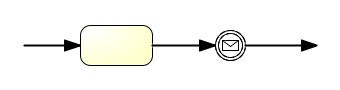
\includegraphics[width=1\linewidth]{chapters/assessment/standard-intermediate-event.png}}
	\caption{Standard Intermediate Catch Event}\label{fig:excerpt-standard-event}
\end{figure}

The first scenario represents the most simple case, that is also natively supported by the BPMN 2.0 specification. When the event occurs after the Event element has been enabled, the event will be received and the process can proceed normally. The use of a standard Intermediate Catch Event does suffice to cover this situation.

\paragraph{Scenario O2: The event does not occur}
\begin{figure}[]
	\myfloatalign
	{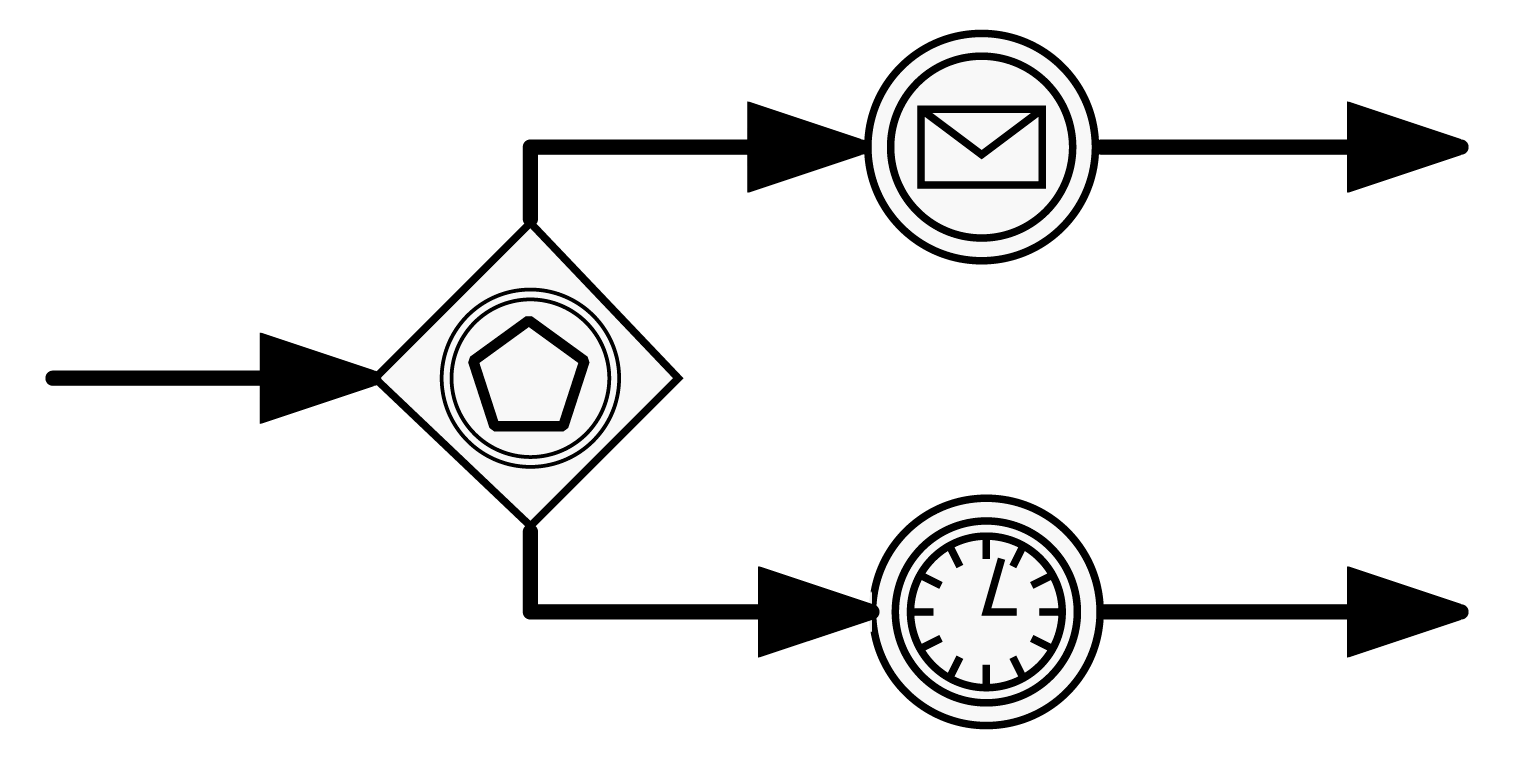
\includegraphics[width=1\linewidth]{chapters/assessment/parallel-timer-event.png}}
	\caption{Intermediate Event with a parallel Timer Event}\label{fig:excerpt-event-with-timer}
\end{figure}
\todo[inline]{alternatively: a receive task with boundary timer event}

In certain situations an event might not occur at all. Given a basic event implementation like in \autoref{fig:abstract-process-with-event}, the process flow will get to a halt once it reaches the Intermediate Catch Event and will not be able to proceed. While, depending on the process design, this might be the desired behavior, in many situations this is not acceptable.

Let's consider a process that is supposed to wait for approval for a certain amount of time and trigger an additional request if the approval has not been issued before the deadline. \autoref{fig:excerpt-event-with-timer} shows how this behavior can be implemented using an Event-based Gateway which puts a Timer Event in parallel to the Intermediate Catch Event. This extension will make sure that a process does not run into a deadlock state if the expected event does not occur.

\todo[inline]{I mention an example, but that example is not exactly illustrated in the process}
\todo[inline]{according to the spec: what exactly will happen to the active catch event once the timer fires?}


\paragraph{Scenario O3: Occurrence between Process instantiation and the enabling of the BPMN event}
\begin{figure}[]
	\myfloatalign
	{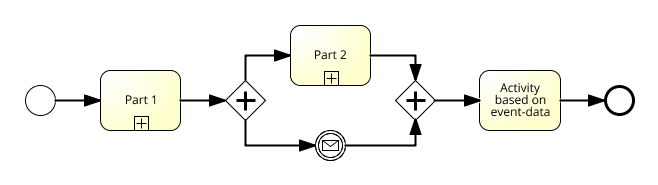
\includegraphics[width=1\linewidth]{chapters/assessment/parallel-gateway-early-subscription.png}}
	\caption{Event Element in parallel process flow}\label{fig:excerpt-parallel-gateway-event}
\end{figure}

In case the event occurs during process execution, but before the BPMN event element is enabled and thus listening for events, the occurrence will not be considered in the execution. The process will get stuck at the Event Process Element as if the event did not happen at all.
To avoid a deadlock in this scenario, a solution is to execute the Intermediate Catch Event in parallel to the rest of the process flow using a Parallel Gateway. This is illustrated in \autoref{fig:excerpt-parallel-gateway-event}. The time of subscription to the event can be controlled by the position of the parallel split: To implement an event subscription right after process instantiation, the Parallel Gateway has to be the first element after the Start Event (that means \textit{Part~1} in the illustration is empty). To implement event subscription at a specific point during process execution, part of the process can execute before reaching the Parallel Gateway. In \autoref{fig:excerpt-parallel-gateway-event}, the event may occur at any time during the execution of the collapsed sub-process \textit{Part~2}. 

\paragraph{Scenarios O4 and O5: Before Process Instantiation}
\begin{figure}[]
	\myfloatalign
	{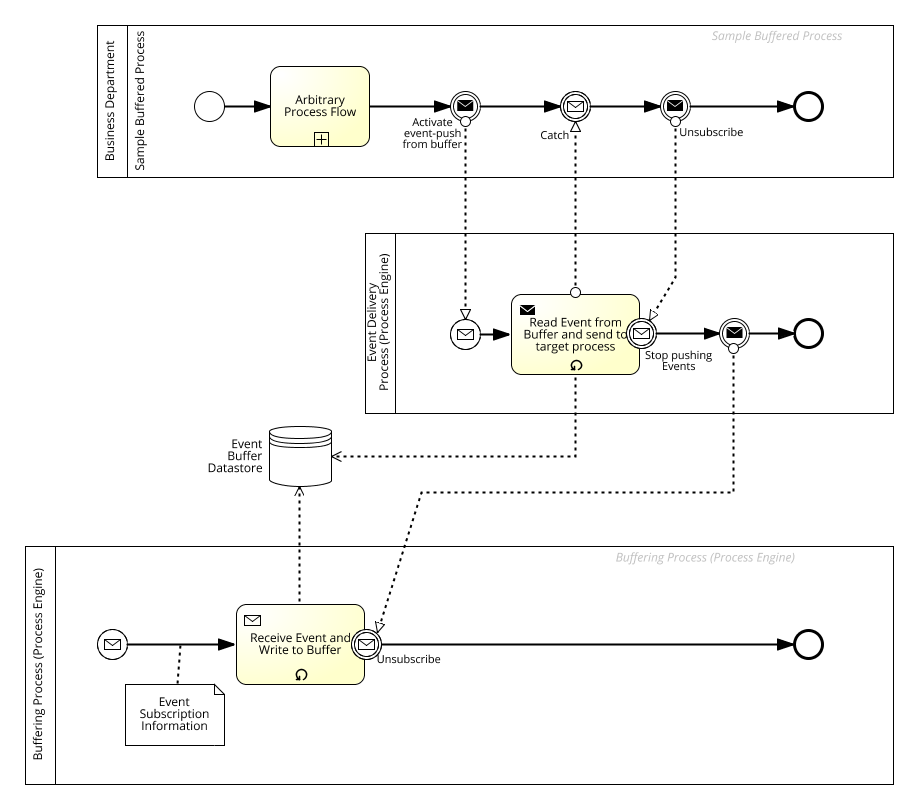
\includegraphics[width=1\linewidth]{chapters/assessment/aux-buffer-process.png}}
	\caption{Event Buffering through an auxiliary Buffering Process}\label{fig:aux-buffering-process}
\end{figure}

Any Events that happen before process instantiation will not be considered in a standard Intermediate Catch Event. That applies to both scenarios, the occurrence between deployment and instantiation (\textit{O4}) and an occurrence time before the deployment of the process in the Process Engine (\textit{O5}).

To create a Process Model that allows to catch an event before the process instance exists, three new elements are introduced: (1) An additional \textit{Auxiliary Buffering Process} that can catch an incoming event, (2) an \textit{Event~Buffer}, a temporary data-store that keeps event data until required by the \textit{Original~Process}, (3) an \textit{Auxiliary Event Delivery Process}, that retrieves events from the buffer and makes them available to the \textit{Original~Process}.
\autoref{fig:aux-buffering-process} reveals the interaction of the \textit{Original Process}, the two auxiliary processes and the data-store. To start listening for an event, the \textit{Auxiliary Buffering Process} has to be instantiated through the a message start event containing the information necessary for the event subscription. The process starts listening for the event and writes the received event to the temporary data-store. 
The given process design is able to handle multiple event occurrences, because the receiving activity is looping. The buffering process terminates once the \textit{Unsubscribe} event is received.

\todo[inline]{how should the ABP be started? manually?}

The \textit{Original Process} can be started any time after the buffering process. In \autoref{fig:aux-buffering-process}, the Intermediate Catch Event has been explicitly split into three events: An initial Send Event to request events, a Catch Event to receive and a final Send Event to signal that no events shall be received anymore.
The initial Send Event instantiates the \textit{Auxiliary Event Delivery Process}, which tries to read from the Event Buffer and deliver the event to the Original Process. Once there is data available in the buffer, it is sent by the sending activity. The central looping activity will retry reading from the buffer until data becomes available and will only be terminated once the \textit{Stop}-event occurs. 
The Original Process can receive the event using a standard Intermediate Catch Event even when the event occurs before the instantiation of \textit{Original Process}, so it handles scenario \textit{O4}. 
Moreover the \textit{Auxiliary Buffering Process} is not bound to a specific event, it works generically with any event information that is passed on to it. For that reason it is also not bound to a specific process deployment and can buffer events even before a process has been deployed, so it handles scenario \textit{O5}.
Given that the buffering process can alternatively be started using an explicit Message Send Event during process execution and the process does not stop listening until the Original Process has received the event, scenarios \textit{O1} and \textit{O3} are also supported.

\todo[inline]{what exactly is passed around|how many instances of each process|overwrite or append to buffer|this is only one solution to do this, one that requires minimal changes in the original process}

\section{Implemention of Early Event Subscription using standard Camunda}\label{ch:assessment-implementation}
The previous chapter has shown that that it is possible to create BPMN models to match each of the Event Occurrence Scenarios, though for the scenarios \textit{O4} and \textit{O5} the solution becomes increasingly complex.
In the next step I investigate the capabilities of Camunda, a modern and actively developed Business Process Engine that is available under an open source license.
Camunda shall be used without any code customization, that means as offered on the website.
The solution presented for the last two scenarios has proven capable enough to handle all Event Occurrence Scenarios, therefor the goal is to implement this solution. It will be necessary to create the two auxiliary processes and a data-store in addition to the original process that makes use of the event buffering.

Two generic sample processes have been modeled for demonstration purposes. \autoref{fig:camunda-example-o3} shows a simple process with an explicit subscription activity to represent the listening to the event after process instantiation but before reaching the Catch Event (Scenario \textit{O3}). It follows a sample activity that takes 15 seconds (implemented using a \textit{Script Task}), the Intermediate Catch Event and another Script Task that displays the content of the received message.
The example for scenarios \textit{O4} and \textit{O5} (see \autoref{fig:camunda-example-o4-o5}) comprises the following elements: After the start event follows an Intermediate Catch Event, then an activity that prints the message of the event to console and last the Process End Event. Both figures show the processes as modeled in the Camunda Modeler.

\begin{figure}[]
	\myfloatalign
	{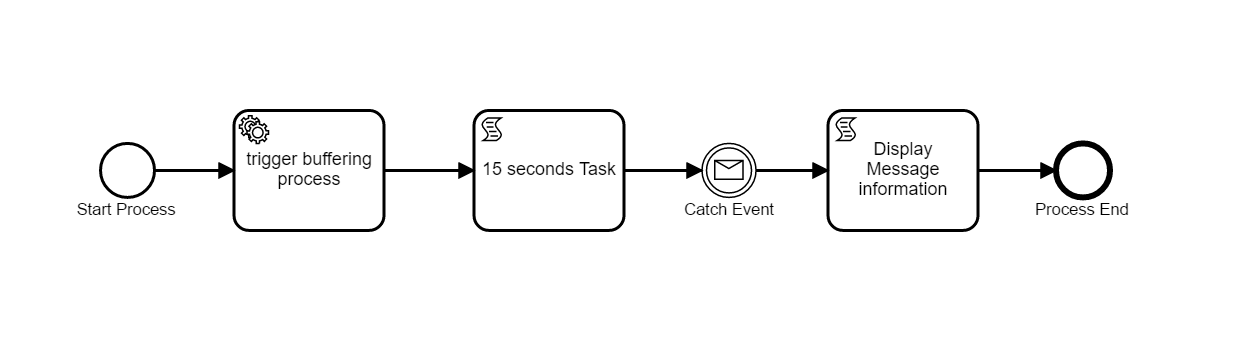
\includegraphics[width=1\linewidth]{chapters/assessment/example-o3.PNG}}
	\caption{Generic Example Process in Camunda for Occurrence Scenario \textit{O3}}\label{fig:camunda-example-o3}
\end{figure}

\begin{figure}[]
	\myfloatalign
	{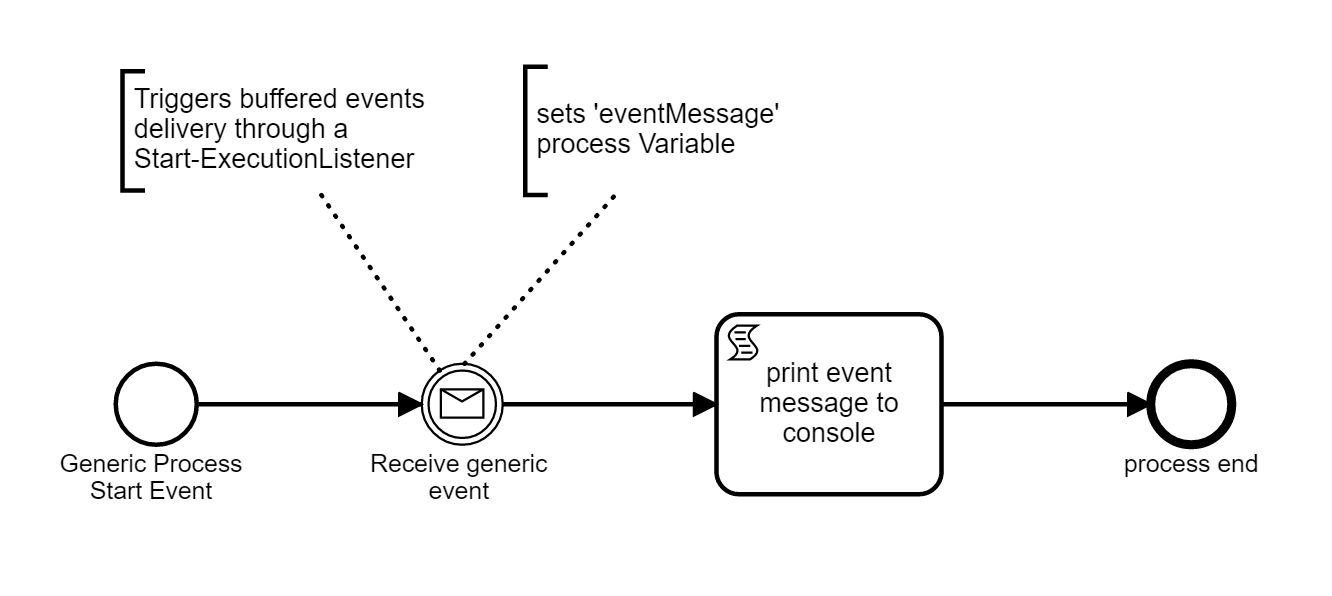
\includegraphics[width=1\linewidth]{chapters/assessment/example-o4-o5.PNG}}
	\caption{Generic Example Process in Camunda for Occurrence Scenarios \textit{O4} and \textit{O5}}\label{fig:camunda-example-o4-o5}
\end{figure}

\paragraph{Auxiliary Buffering Process}
The task of this process is to subscribe to a CEP Platform using a provided event query and start listening for events. Any incoming event must be stored in a data-store (\textit{Event Buffer}).
UNICORN, an Esper-based academic event processing platform, will be used in this example.
A local MySQL database has been chosen for buffering the event data because it's freely available, quick to set up, offers standardized access via SQL queries and Java connectors and will persist data to the local harddrive by default. As UNICORN also requires an SQL database, the MySQL instance can be used in both cases.

\autoref{fig:camunda-aux-buffering-process} shows the final Buffering Process modeled in the Camunda Process Modeler. The process can be instantiated by issuing a \textit{Buffering Task} message. This message must contain three data fields: \textit{processDefinitionId}, to know which process definition the buffered messages belong to; \textit{messageName}, the name of the message event within the process; \textit{query}, the event query in the Esper Query Language.
Camunda will make the message data automatically available in the process instance as process variables, so they can be used during the execution of the Buffering Process.
After instantiation, the process reaches the activity \textit{Subscribe to Event Source}, a \textit{Java Service Task} that executes a HTTP call to the UNICORN platform. That call registers the event query in UNICORN. \todo[inline]{it tells unicorn its own instanceId, so that unicorn can correlate events to that exact instance}
Afterwards, the process reaches the receiving activity \textit{Wait for unsubscribe event} that will terminate the process as soon as the \textit{Unsubscribe} event has been received.
As long as this activity is active, events can be received through the attached Non-Interrupting Boundary Event. Incoming events have a field \textit{eventBody}, which contains the event information and becomes available through a process variable with the same name. \todo[inline]{does the message from UC have a field 'eventBody'?}
The boundary event triggers the service task \textit{Write eventBody to datastore}, which takes the data from the process variable and writes it to the MySQL Database Instance (\textit{Global Event Buffer}).

\begin{figure}[]
	\myfloatalign
	{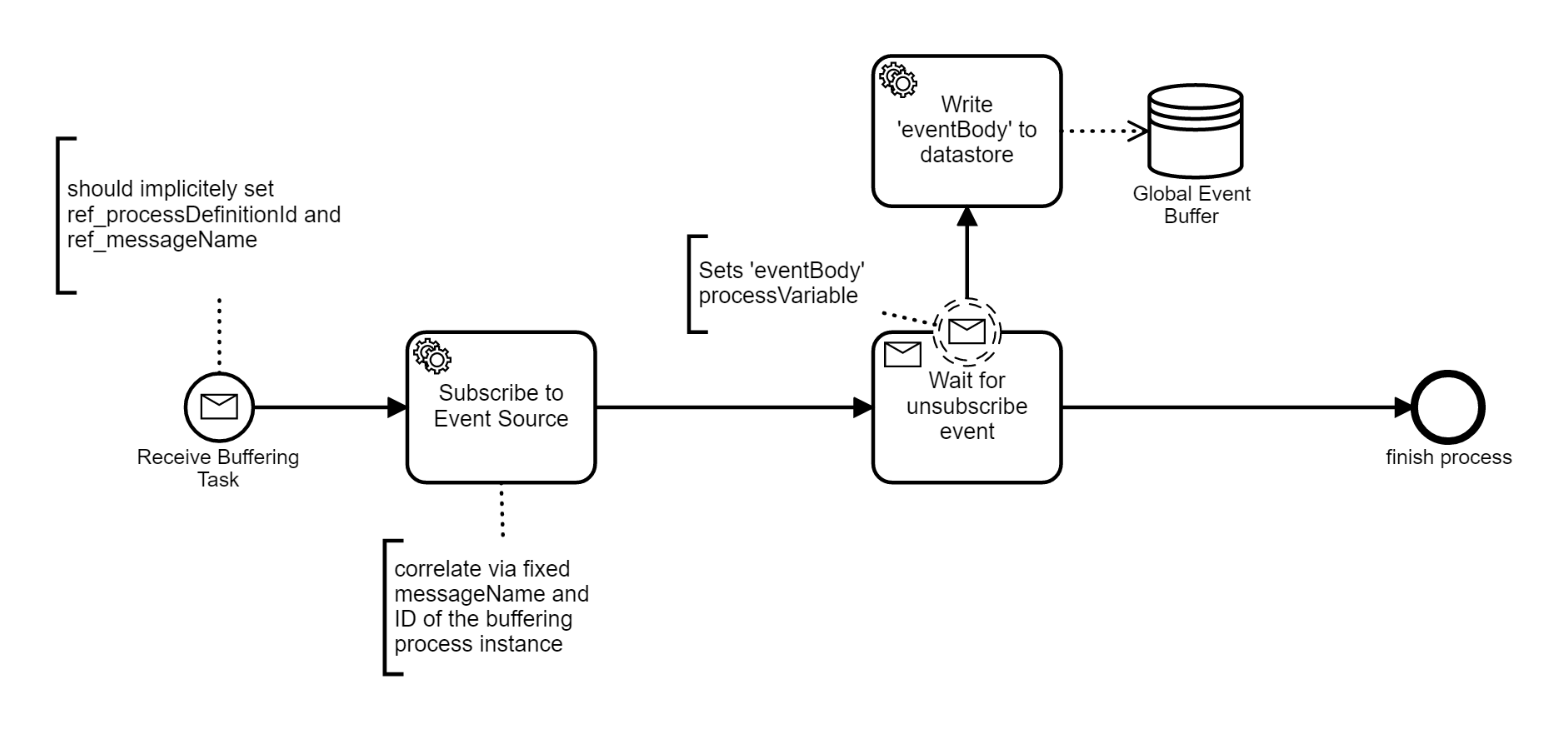
\includegraphics[width=1\linewidth]{chapters/assessment/buffering-process.PNG}}
	\caption{Auxiliary Buffering Process in the Camunda Modeler}\label{fig:camunda-aux-buffering-process}
\end{figure}

\paragraph{Auxiliary Event Delivery Process}
The delivery process (see \autoref{fig:camunda-aux-event-delivery}) reads the latest data from the buffer and sends it to the process instance. It can be started with a message that contains the \textit{processInstanceId} and the \textit{processDefinitionId} of the requesting process and the \textit{messageName} of the Message Event that is requested from the buffer.
A \textit{Delay} Timer Event has been inserted to make sure that the receiving process is already in listening state, the execution happens asynchronously.
It follows the service task \textit{Retrieve event from buffer}, which executes Java code to read from the MySQL Database \textit{Event Buffer} and store the event information in a process variable named \textit{eventMessage}.
The content of that process variable is sent to the \textit{Original Process} in the Send Event, afterwards the execution is finished.


\begin{figure}[]
	\myfloatalign
	{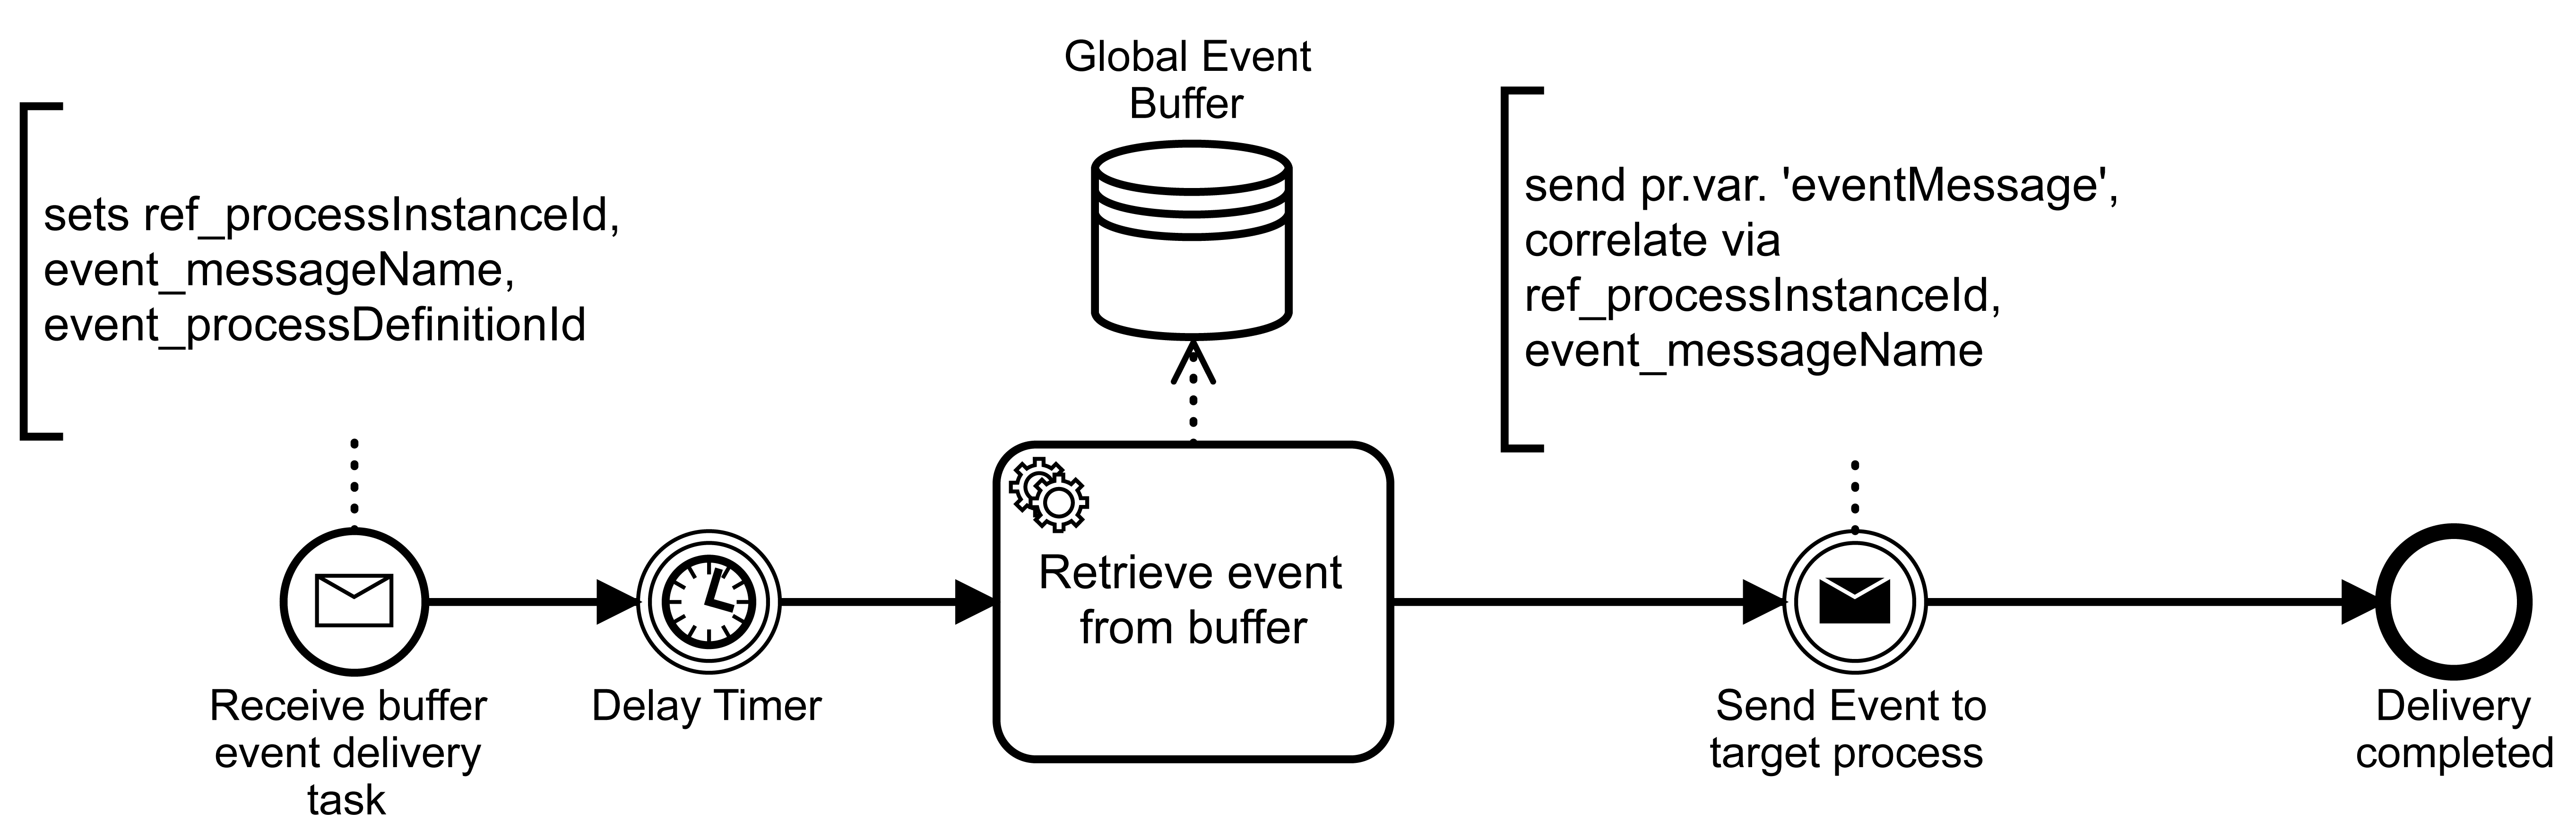
\includegraphics[width=1\linewidth]{chapters/assessment/buffer-delivery-process.PNG}}
	\caption{Auxiliary Event Delivery Process in Camunda Modeler}\label{fig:camunda-aux-event-delivery}
\end{figure}


\paragraph{Interaction of the Processes}
In this implementation of flexible event subscription, the action of subscribing to the event source and the reception of events in the Original Process are splitted into two separate parts, each supported by an auxiliary process.
To initiate the subscription at the event source, the Auxiliary Event Buffering process has to be started.
For scenario \textit{O3}, this happens through an extra activity (\textit{Trigger Buffering Process}) during process execution, so that events after process instantiation are received by the Buffering Process.
In scenarios \textit{O4} and \textit{O5}, the subscription and thus the instantiation of the Buffering Process must happen before the instantiation of the Target Process. As there is no such mechanism in the standard Camunda Process Engine, the Buffering Process must be started by hand, providing the \textit{processDefinitionId}, the \textit{messageName} and the \textit{eventQuery}.

Now that the \textit{Buffering Process} is running, any events matching the query will be stored to the buffer.
When the Target Process reaches the Catch Event, a request for buffered events is sent as a message to trigger the \textit{Auxiliary Event Delivery Process}.
This message is sent using a short piece of Java code that gets executed when the Catch Event is reached. 
The code is invoked by a Start ExecutionListener attached to the Catch Event. ExecutionListeners are offered by Camunda to execute own Java programs before or after relevant events during process execution, like the execution of an element in the process.
While the Original Process will now start listening for the desired events, the Event Delivery Process will send the buffered events as messages to the Original Process.

If no events have been received yet, all the involved processes remain active: the Buffering Process will keep listening for an external event. The Delivery Process will send an event to the Original Process as soon as there is one in the buffer. The Catch Event in the Original Process will keep listening for an Event.

\todo[inline]{the termination of the processes is not yet implemented in Camunda}
\todo[inline]{get wording straight: Original process, target process, requesting process, main process | also always italic or never}

\missingfigure{overview of the 3 processes, mysql and UNICORN}

\todo[inline]{note that this is an investigative implementation that matches exactly the given use-case and is not meant to be used in production. It is neither flexible nor robust enough for that purpose, but suits very well in understanding the capabilities and the shortcomings of BPMN and Camunda when it comes to handling the Event Occurrence Scenarios}


\section{Discussion}
The goal of this chapter was to get a better understanding of the capabilities of the tools when it comes to covering all event occurrence scenarios. 
Even though is has proven possible to to implement a flexible event subscription time using standard BPMN 2.0 and Camunda, the success comes at a cost.
The downsides of the presented approach are presented in the following.

It was necessary to create two generic auxiliary processes for event buffering, to connect to a MySQL data-store and use ExecutionListeners to execute custom Java code in Camunda to cover all scenarios, \textit{O1} to \textit{O5}.

\todo[inline]{give them short names for reference? Or make one of them Requirement 5}


\paragraph{Missing automatic subscription handling\newline}

In the presented process models, separate process elements had to be added to handle event subscription and initiate event delivery. 
That conflicts with requirement \textit{R2}, which states that the subscription and un-subscription must be automatically handled by the process engine.
For the scenarios \textit{O4} and \textit{O5} the Buffering Process has to be triggered manually, because it must be executed before the target process is running. Camunda does not handle external event subscription itself, especially not before the process is running.

\paragraph{Additional model complexity\newline}

As additional process elements have to be added to handle event subscription and delivery, the models become more complicated and are less concentrated on the business case.
\todo[inline]{there could be a requirement that states that there should be no additional process elements unless there is an explicit subscription time}

\paragraph{Buffering is an IT Task\newline}

The auxiliary processes are not business tasks and are thus not suited to be modeled in BPMN.
Desired functionality can be put into Camunda BPMN models thanks to its flexibility to use Java code in Service Tasks or Event Listeners, but naturally the full functionality of the Event Buffer cannot be expressed using BPMN.
\todo[inline]{what exactly is the issue here?}

\paragraph{Added load on the Process Engine\newline}

Because of the aux processes, two additional processes have to be deployed in the process engine and are potentially running in parallel to any given process instance. For each Event Element used in a process the engine has to run an instance of the Buffering Process and, eventually, an instance of the Buffer Delivery Process.
That puts additional load on the process engine, which might prevent business critical processes from executing delay-free.

Even when the number of deployed and running auxiliary processes can be reduced through further optimizations there remains an event-management overhead as every event has to be handled twice: once when it is stored in the buffer and once when it's delivered to the target process.

\paragraph{Hidden Performance Limitations of the Process Engine\newline}

Given the large amount and high frequency in that events can occur in reality, optimal performance is required for an event-buffering module.
Running essential parts of the buffering within the process engine might pose performance limitations that cannot be influenced without tempering with the process engine code.



\cleardoublepage%************************************************
\chapter{Flexible Event Subscription in BPMN}\label{ch:flexibleeventsubscription}
%************************************************

- Introduce a new concept. three pillars: bpmn-x, process engine behavior, event handling api
\todo[inline]{write intro}

\missingfigure{The concept for flexible event subscription involves three modules: A BPMN extension, enhanced process engine behavior and buffered event handling.}
\label{fig:concept-modules}

\section{BPMN Extension}\label{ch:bpmnx}

% maybe cite braun2015behind

The extensibility mechanism of the \ac{BPMN} allows to extend standard process elements with additional attributes, while maintaining conformity with the BPMN core~\cite[p.\,44]{bpmnspec}.
Extensions are specified through an external definitions file and can be included into a BPMN process model by reference.

\todo[inline]{write a little more about bpmn extensibility, then section structure}

- utilizing this mechanism, we propose a BPMN extension for flexible event subscription

-> refer to as befes? or just "the extension"
- structure of this section: overview (initial understanding of the extended notation and the semantics), usage documentation(, detailed execution semantics?)

\subsection{Overview}
This section introduces a novel BPMN extension for incorporating event subscription semantics in business process models.
The extension develops around the addition of subscription-related attributes to the BPMN \textit{Message} type. Based on the additional information, subscription and un-subscription for message events is handled automatically by an especially adapted process engine.
The added attributes are \textit{EventQuery}, \textit{SubscriptionTime} and \textit{BufferPolicies}:
\textit{EventQuery} contains an arbitrary query string; \textit{SubscriptionTime} defines when the subscription should happen; \textit{BufferPolicies} is a complex type which influences the behavior of the related event buffers.
Only \textit{EventQuery} is a mandatory parameter, all others will fall back to default values if not provided.
An overview of all possible fields, values and their defaults is provided in \autoref{tab:bpmn-extension}.

% variables in the event query

The presented extension is to be used in connection with intermediate catch events, boundary events and receive tasks through their direct or indirect association with the message element.
Additionally, the \textit{Event Subscription Task}, an extension of the \textit{Task} is introduced. It adds a single additional attribute \textit{messageId} to \textit{Task} and can thereby be used to manually trigger the subscription for the associated message element as part of the execution flow of a process.
%- for the others, the subscription and unsub from the event source is managed implicitly by the underlying infrastructure
By the use of the \textit{subscriptionTime} variable, the event subscription can be issued before the process flow reaches the event element and listens for the message. %bpmn event element is listening.
Any messages that arrive before the event element is active are temporarily stored and will be delivered to the catch event or receive task once it is active.
These storages as referred to as \textit{Event~Buffers}. By default, they store the latest message they receive, though the behavior can be adjusted using the \textit{BufferPolicies}.
The extension elements are illustrated through a UML-representation in \autoref{}, the formal XSD-Schema is available in the appendix, \autoref{lst:xsd-flexsub}.\todo[inline]{fix ref}

%- it is required that the infrastructure is prepared to execute extended processes accordingly, ref chapter
% though, theoretically, every message can be extended with the attributes, the subscription is only managed for the elements...

\missingfigure{UML-Diagram of BPMN extension: task>expl subscr task; message > messageeventdef > interm catch event; message > receive task}


\begin{table}
	\myfloatalign
	\begin{tabularx}{\textwidth}{p{0.3\linewidth} p{0.515\linewidth} c}
		\toprule
		\tableheadline{Attribute Name} & \tableheadline{Value Options (\underline{default})} & \tableheadline{Req.} \\ 
		\midrule
		EventQuery & any query string & y \\
		SubscriptionTime & process-deployment,\newline process-instantiation,\newline manual, \underline{element reached} & n \\
		BufferPolicies & Complex Type (see below) & n \\
		
		\midrule
		\tableheadline{bufferPolicies}  \\
		\midrule
		
		LifespanPolicy & string in ISO time-span format OR '\underline{infinite}' & n \\
		ConsumptionPolicy & \underline{reuse}, bounded-reuse(n), consume & n \\
		SizePolicy & positive integer, \underline{1}, 0 means infinite & n \\
		OrderPolicy & \underline{FIFO}, LIFO & n \\
		
		\bottomrule
	\end{tabularx}
	\caption[]{Available attributes of <subscriptionDefinition> in the BPMN extension for flexible event subscription}  \label{tab:bpmn-extension}
\end{table}

\subsection{Documentation}

> why everything is added to the message element


Semantically, the \textit{Message} type is most suited to be extended with subscription information.

% receiveTask.messageRef; boundaryEvent.catchEvent.(message)eventDefinition.messageRef; intermediateCatchEvent.catchEvent.(message)eventDefinition.messageRef
Each of the three elements references a BPMN \textit{Message}, the common denominator for communication within and across business processes.

\todo[inline]{mention that others have extended the events instead, but this proposal goes another way}

\todo[inline]{explain that the Message is a common element in BPMN models. It is the main generic type used for communication, collaboration.
	The proposed extension to the Message type is only to be used by Message Receive situations in Intermediate Catch Event, the Boundary Catch Event and the Receive Task.}

By specification, \textit{tMessage} comprises an attribute \textit{name}, the name of the message, and \textit{itemRef}, the reference to a BPMN \textit{ItemDefinition}. Additionally, it inherits all attributes from the BPMN \textit{RootElement}.
In the following, the required additional attributes will be explained one after the other. A complete list is available in \autoref{tab:bpmn-extension}. The goal is to retain a stand-alone model that contains all information necessary to execute the subscription to the event source.

- information is added to <subscriptionDefinition>

%\subsubsection{Introducing Event Buffers}
%Any event message that occurs before reaching the event element but after the time of subscription will be kept in a buffer by the system.
%In its simplest version, the buffer is of length 1, that means it stores exactly one message received from a CEP platform. It always stores the latest message. When a newer message arrives, the old one is replaced in the buffer.
%\autoref{ch:bpmnx:bufferpolicies} introduces a set of advanced buffer policies to adapt this behavior further.
%\todo[inline]{By default, there is no interference between the buffers of different messages, process instances or processes. Each buffer instance will contain the latest information as if it was the only buffer in the system. Performance improvements to avoid duplicate buffer content will be managed by the system without explicit action by the user. Section ... later introduces a shared, more complex usage scenario of the event buffers.}

\subsubsection*{Adding basic subscription information}\label{ch:bpmnx:basic}

For a subscribe operation, we consider the event~query, the platform address and optionally authorization information of the CEP~platform.
This extension assumes that only one event engine is in use, so that access information can be configured in a central configuration store for the current process execution environment and not redundantly for each message.
The event query instead needs to be specified for every message and is added to the model as an extension attribute \textit{eventQuery} of type \textit{string}, which should contain the full query as interpretable by the CEP platform.

A similar approach has been taken by X and Y, who aim at enriching BPMN models with subscription information without considering the time of subscription specifically.
\todo[inline]{Find this source; explain what they do (different)}

Given this first fundamental part of the BPMN extension, it is possible to execute the subscription, but the time of subscription cannot be influenced.

\subsubsection*{The time of event subscription modeled in BPMN}\label{ch:bpmnx:subscriptiontimes}

This section specifically addresses the requirement \textit{R1.1}, aiming to provide a flexible event subscription time to be selected for each BPMN message when designing an event-driven process.
Two different means are to be offered to support all subscription times demanded by \textit{R1.1}: Firstly, the subscription can happen in the background. Alternatively, the subscription can be modeled explicitly as a flow-element in the process.
It is a task of the process design phase, to elaborate the correct time of subscription necessary for the use case.

The subscription will be executed automatically by the system based on the information given in the BPMN model. Further information on the exact execution flow is provided in chapter~XY.

\todo[inline]{Time of un-subscription also must be clarified in bpmnx}


\paragraph{Subscription time as part of the BPMN Message element\newline}
To provide the Process Designer with a simple but powerful tool to influence the time of event subscription, a field \textit{subscriptionTime} is added the BPMN message element. 
The field can take one of the following values: \textit{process-deployment}, \textit{process-instantiation}, \textit{manual}, \textit{element-reached}. The last option is the default option, intepreting the standard BPMN semantics.
Note that a \textit{subscriptionTime} set to \textit{element-reached} will remain without effect if an explicit subscription task for the same event was executed before the event is reached.

\todo[inline]{For each of the options: Define exactly (according to BPMN spec or standard literature), when in the flow the subscription is executed.}

In motivating Example~1.1, it is necessary to issue the subscription to the Eurotunnel event as early as possible to make sure that data is available and the process execution is not delayed.
Using the BPMN extension, the use case can be implemented by defining the event query and the subscription time in the BPMN model. \todo[inline]{show what that would look like in the example. Maybe some XML?}

\paragraph{The event subscription task\newline}
As an alternative to specifying the subscription time using the extension field \textit{subscriptionTime}, an extension to the BPMN \textit{Task} type is proposed. \todo[inline]{it follows the ideas presented in ... but through referencing the message element}
Other than \cite{mandal:2017} 



\missingfigure{Example 2 using an explicit subscription task}

The extended task is used to execute the subscription explicitly as part of the process flow.
A field \textit{messageId} is added to the service task to establish a reference between the activity and the message definition.
As introduced in section~\autoref{ch:bpmnx:basic}, the extended BPMN Message definition contains the information necessary to issue the subscription to an event source.
Once the Explicit Subscription Task is activated, the subscription for the referenced message is issued. 

Modeling the event subscription in an explicit task can be necessary when the subscription depends on the result of another activity. In that case, the subscription cannot be issued on process instantiation, because the necessary information is not yet available. Instead, an early subscription can be implemented using the extended service task.
Apart from this particular use case, the explicit subscription task enables the Process Designer to place the subscription flexibly in the process flow and give her full control over the time of subscription.

\todo[inline]{As an improvement to the options for subscription time, there could be an option "ASAP", so that the process engine issues the subscription automatically as soon as the required process data becomes available}

If both tools, the extension field \textit{subscriptionTime} and the explicit subscription task, are used for a single BPMN message, the earlier subscription of the two will be executed, the second subscription will have no effect.
That means for example if the \textit{subscriptionTime} is set to \textit{event reached} and an explicit subscription task is inserted before the event element, then the subscription will be executed at the time the explicit subscription task is active.
If \textit{subscriptionTime} is set to \textit{Process Deployment}, then the subscription will happen at that time and the explicit subscription task will remain without effect.
In case neither of the two is used, the system falls back to the BPMN default and executes the subscription when the event element is reached.

\subsubsection{Using Process Variables in Event Queries}

% also see bpmn2 spec 10.3 pp. 233ff.

As shown in example~1.2, it can be the case that the current values of process data must be dynamically used in an event query. \todo[inline]{missingref}
Therefore, the name of the dataObject should be part of the event query. At the time of subscription, the mentioned variable is dynamically replaced by its current value.
The exact notation for including process variables in event queries may vary depending on the employed query language so that it does not interfere with any existing notation schemes.
For the use with the Esper EPL, the following is suggested: The exact name of the variable has to be surrounded by curly brackets and preceded by a \textit{\#} character: \textit{\#\{VARIABLENAME\}}.
This notation is inspired by the usage of substitution parameters in SQL queries that are embedded in Esper EPL. They take a similar form, though using a \$ sign\footnote{see~\textit{5.13.1. Joining SQL Query Results}, \url{http://www.espertech.com/esper/release-5.3.0/esper-reference/html/epl_clauses.html}, accessed 2017-08-13}.

\todo[inline]{brief recap of the example and show query using the variable. considering the value is stored in the dataObject ".."}
\textit{SELECT lat, lng from GPSUPDATE where truckid = \#\{truckid\} }.

The use of dynamic process variable values introduces an additional complexity: Depending on the time of event subscription, the value of the process variable might not yet be available.
\todo[inline]{only if subscriptionTime not 'on depl'}
\todo[inline]{What does this mean for the process designer? A model that can take a state in that a subscription shall be issued, though the data is unavailable, is invalid. When will an error occur? }


\subsubsection{Advanced Buffer Parameters}\label{ch:bpmnx:bufferpolicies}

\paragraph{Lifespan of buffered events\newline}

The \textit{LifespanPolicy} allows to specify after which timespan elements in the buffer should be deleted. Timespans are defined using the ISO8601 notation for time intervals\footnote{see \textit{Date and time format - ISO 8601}, \url{https://www.iso.org/iso-8601-date-and-time-format.html}, accessed 2017-08-13}. 
The default value is \textit{infinite}.

\todo[inline]{überleitung zu example}
Example~1.1 is implemented by setting the \textit{subscriptionTime} to \textit{process-deployment}, which means that there can be an infinite time difference between the action of subscribing to the event source and the reaching of the event element in one of the instances. \todo[inline]{ref example}
In case events are not published in a longer time, for example due to technical fault at the event producer, the buffer will contain older events that might not be relevant anymore.
Using the \textit{LifespanPolicy}, the process designer can express, that events should be deleted from the buffer after a certain period of time and thus avoid outdated information. The buffer is maintained automatically by the system.
That of course comes at the price that the process has to remain in waiting state until a new event message arrives.

\paragraph{Consumption Behavior\newline}

So far, the event buffers can be used isolated from each other. There is no interference between buffer instances and events are not removed from the buffer after retrieval.
While for most use-cases this behavior is sufficient, more detailed control over the buffer can be desirable when a given message is accessed multiple times. More precisely, if an event element is activated multiple times or multiple elements reference the same \textit{Message} element, then the consumption behavior must be clear.
Not always is it wanted, that events remain in the buffer after retrieval.
An additional parameter \textit{ConsumptionPolicy} is introduced which can take the values \textit{consume}, \textit{reuse}(default) and \textit{bounded reuse(n)}.
While \textit{reuse} denotes the behavior that is already known, \textit{bounded reuse(n)} will allow an element to be retrieved exactly \textit{n} times. \textit{n} has to be replaced by an integer value greater 0.
The option \textit{Consume} will remove an element from the buffer immediately after it has been retrieved for the first time, it is therefor equivalent to \textit{Bounded Reuse(1)}.

\todo[inline]{can still be clearer}


\begin{figure}[]
	\myfloatalign
	{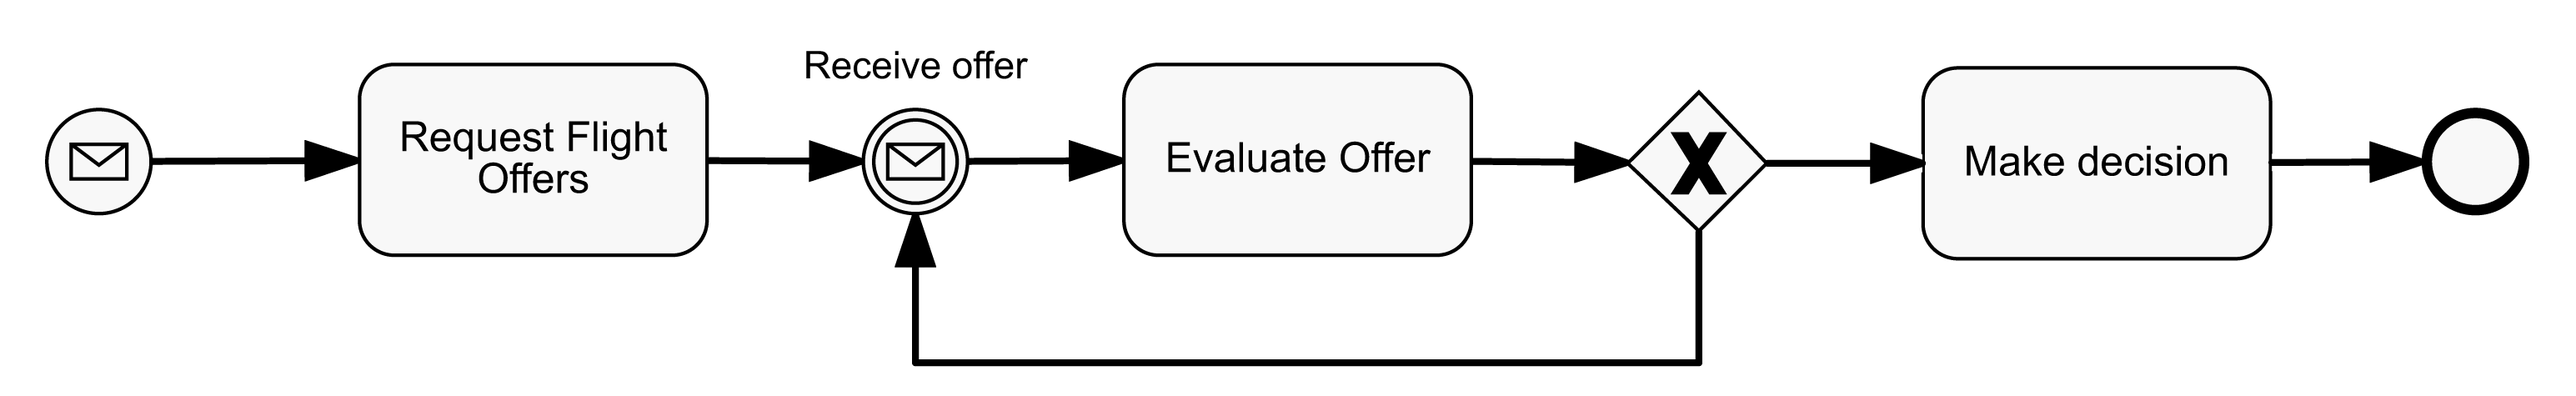
\includegraphics[width=1\linewidth]{chapters/concept/bpmnx/FlightBooking.png}}
	\caption{Flight Booking process using a consuming buffer}\label{fig:example-flightbooking}
\end{figure}

\todo[inline]{write about the examples}

- given the option to consume from the buffer, it will now make a difference if the same buffer is accessed multiple times.
- there are two scenarios to access the same buffer: (1) multiple times in the same instance, (2) multiple times because of parallel instances, (3) multiple times because of a shared buffer across processes
- before proceding, we need to be clear about the buffer scope: it depends on the time of subscription. (1) after instantiation: buffer only instance-wide; (2) on pr depl: buffer reused across all instances; (3) buffer reused across all processes if messageId and query are the same.

\begin{figure}[]
	\myfloatalign
	{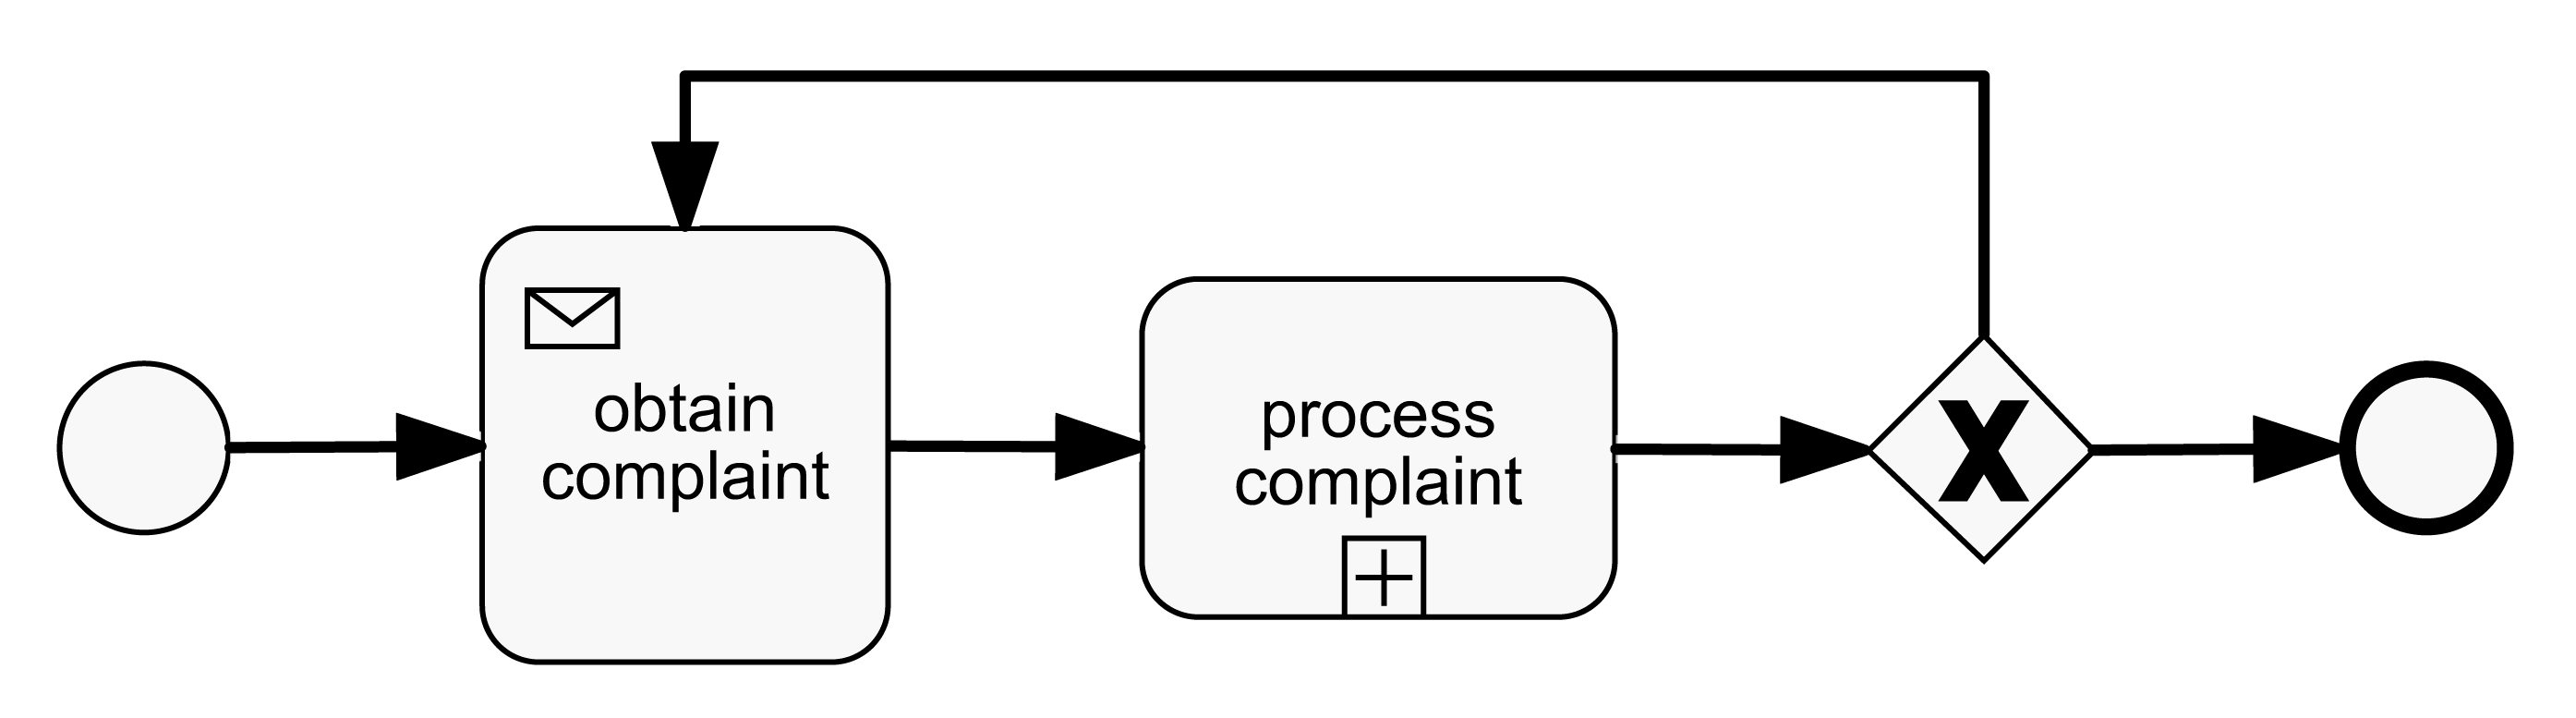
\includegraphics[width=1\linewidth]{chapters/concept/bpmnx/ComplaintProcessing.png}}
	\caption{Shared consuming buffer in Complaints Handling}\label{fig:example-complaints}
\end{figure}

\paragraph{Buffer Size and Order Policy\newline}

- two additional buffer policies: \textit{SizePolicy}, \textit{OrderPolicy}, default values
\todo[inline]{write text for given keypoints}

- what if messages are defined in different ways? => I want to reuse the buffer between processes, but the message definition (especially cep query) are not the same. how will the system behave?

\paragraph{Interplay of Event Queries and Buffers}

// even with the simplest settings

Modern event query languages are feature-rich and offer a large set of expressions to filter events from incoming streams. \todo[inline]{ref background}
The introduced basic event buffer can be used in connection with any desired event query and will store the latest output of that query.
These two features together suffice to implement even more complex use-cases: Query windows of length \textit{n} can be used to keep multiple events in the buffer, filter expressions allow to keep a subset of all events based on their attribute values, multiple streams can be joined together.
As soon as the process flow reaches an event element, the latest CEP message is retrieved from the buffer. It is not consumed, that means a second event element that references the same BPMN Message will reuse the information from the buffer.
If no information is available in the buffer, the flow element will remain in the waiting state until a message is received. Then, the process flow proceeds as usual.

\subsection{Execution Semantics}

%************************************************
\section{Automatic Subscription Handling}\label{ch:automaticsubscription}
%************************************************

After defining the notation and functionality provided to the user through the BPMN extension for flexible event subscription, this chapter describes the changes necessary to the software infrastructure to implement the execution semantics.
The concept requires that all subscription operations and event handling is executed by the system itself, solely based on the extended BPMN model.
Changes are necessary to both, the event processing module and the process engine. This chapter attempts to keep the change descriptions general so they can be applied to any common process engine and event processing platform.
The first section describes the necessary extension to the event processing so that a delayed delivery of events is supported.
The following \autoref{ch:extendedprocessengine} specifies the changes necessary to the behavior of the process engine as the connecting element between the BPMN model and the event processing platform.


\subsection{Buffered Event Processing}\label{ch:bufferedcep}
When reduced to the basics, a standard event processing platform works as follows: The user subscribes to events providing an event query and a notification-path. The platform responds with a unique identifier for that subscription.
Whenever an event occurs that matches the provided query, the platform issues a notification to the notification-path. Subscriptions can be deleted through their unique identifier.
These two operations, \textit{subscribe} and \textit{unsubscribe}, make the fundamental \acs{API} of a CEP platform~(see \autoref{ch:bg:cep}).

\paragraph{An API for buffered event processing}
The novel BPMN extension for flexible event subscription allows to issue a subscription to an event source well before the events ought to be delivered to the process instance. The introduction of an event buffer as a separate entity between the notification-recipients and the event query makes an adaptation of the API necessary.
In the following, we propose an API for buffered event processing which provides the functionality necessary to implement the execution semantics specified in the BPMN extension. Note that the proposal is not restricted to a certain kind of technology or protocol to implement the API.

Firstly, the \textit{subscribe} operation has to be available in two steps:

\begin{aenumerate}
	\item \textit{registerQuery(queryString[, bufferPolicies]): queryId}\newline
	The call registers an event query in the CEP platform and instantiates a buffer. Matching events will be held in the buffer according to the specified  policies. It returns a unique identifier to that new query registration and hence for the connected buffer. That identifier must be used to modify the query later.
	
	\textit{bufferPolicies} is an optional parameter which is provided as an object with four possible fields: \textit{LifetimePolicy}, \textit{ConsumptionPolicy}, \textit{SizePolicy}, \textit{OrderPolicy}. Refer to \autoref{ch:bpmnx:bufferpolicies} for a detailed specification of the semantics and possible values of the parameters. If \textit{bufferPolicies} is not or only partly specified, the system should fall back to the denoted default values.
	
	\item \textit{subscribe(queryId, notificationPath): subscriptionId}\newline
	Initiates the delivery of notifications for a given queryId to a notification recipient.
	The recipient is specified through the \textit{notificationPath}, the full address of the entity that is supposed to receive the message.
	Notifications are delivered asynchronously as soon as they are available. If the buffer is not empty, a message will be sent right after the \textit{requestEvents} call.
	A similar operation, \textit{addNotificationRecipient}, is available in existing CEP platforms. It adds a notification recipient to a query that is already registered in the platform. The difference is in the delivery of the first buffered message: \textit{requestEvents} sends out the message from the buffer, \textit{addNotificationRecipient} will send out notifications only for future query output.
\end{aenumerate}\label{def:apiextension-subscribe}

\noindent A similar situation holds for the un-subscribe operation: Given flexible event subscription, the operation must comprise of two steps:

\begin{aenumerate}
	\setcounter{enumi}{2}
	\item \textit{unsubscribe(subscriptionId)}\newline
	Removes a notification-recipient for a given query-id. Note that the buffer and query instance remain intact, so that other recipients can still subscribe.
	\item \textit{removeQuery(queryId)}\newline
	Completely deletes the query and its buffer, so that no notifications are sent out any longer. 
\end{aenumerate}\label{def:apiextension-unsubscribe}

\noindent
All four methods must be available to execute a subscription before process deployment.
The query must be registered using \textit{registerQuery} before the process instance, and hence the notification-path, is available. For each process instance, a subscription can be issued individually using \textit{subscribe} and thereafter, the notification-recipient can be removed with \textit{unsubscribe}.
The query and its buffer will remain active even after any single instance has terminated. When the process gets un-deployed, the query can be deleted using \textit{removeQuery}.
%\autoref{ch:extendedprocessengine} describes the steps in detail.

\todo[inline]{show the steps with sample data from one of the examples}


\paragraph{Architectural options}

Three options are considered to implement the explained functionality~(\autoref{fig:buffered-event-handling-architecture}). 
(a) It can either be implemented by adopting the CEP platform itself, (b) by implementing a separate middleware between process engine and CEP platform, (c) or by implementing a buffering module as part of the process engine.
Which of the three options suits best has to be evaluated for the given use-case and existing infrastructure. In some cases it might not be possible to adapt the code of process engine or event processing platform, which leaves a separate middleware as the only choice.

\begin{figure}[]
	\myfloatalign
	{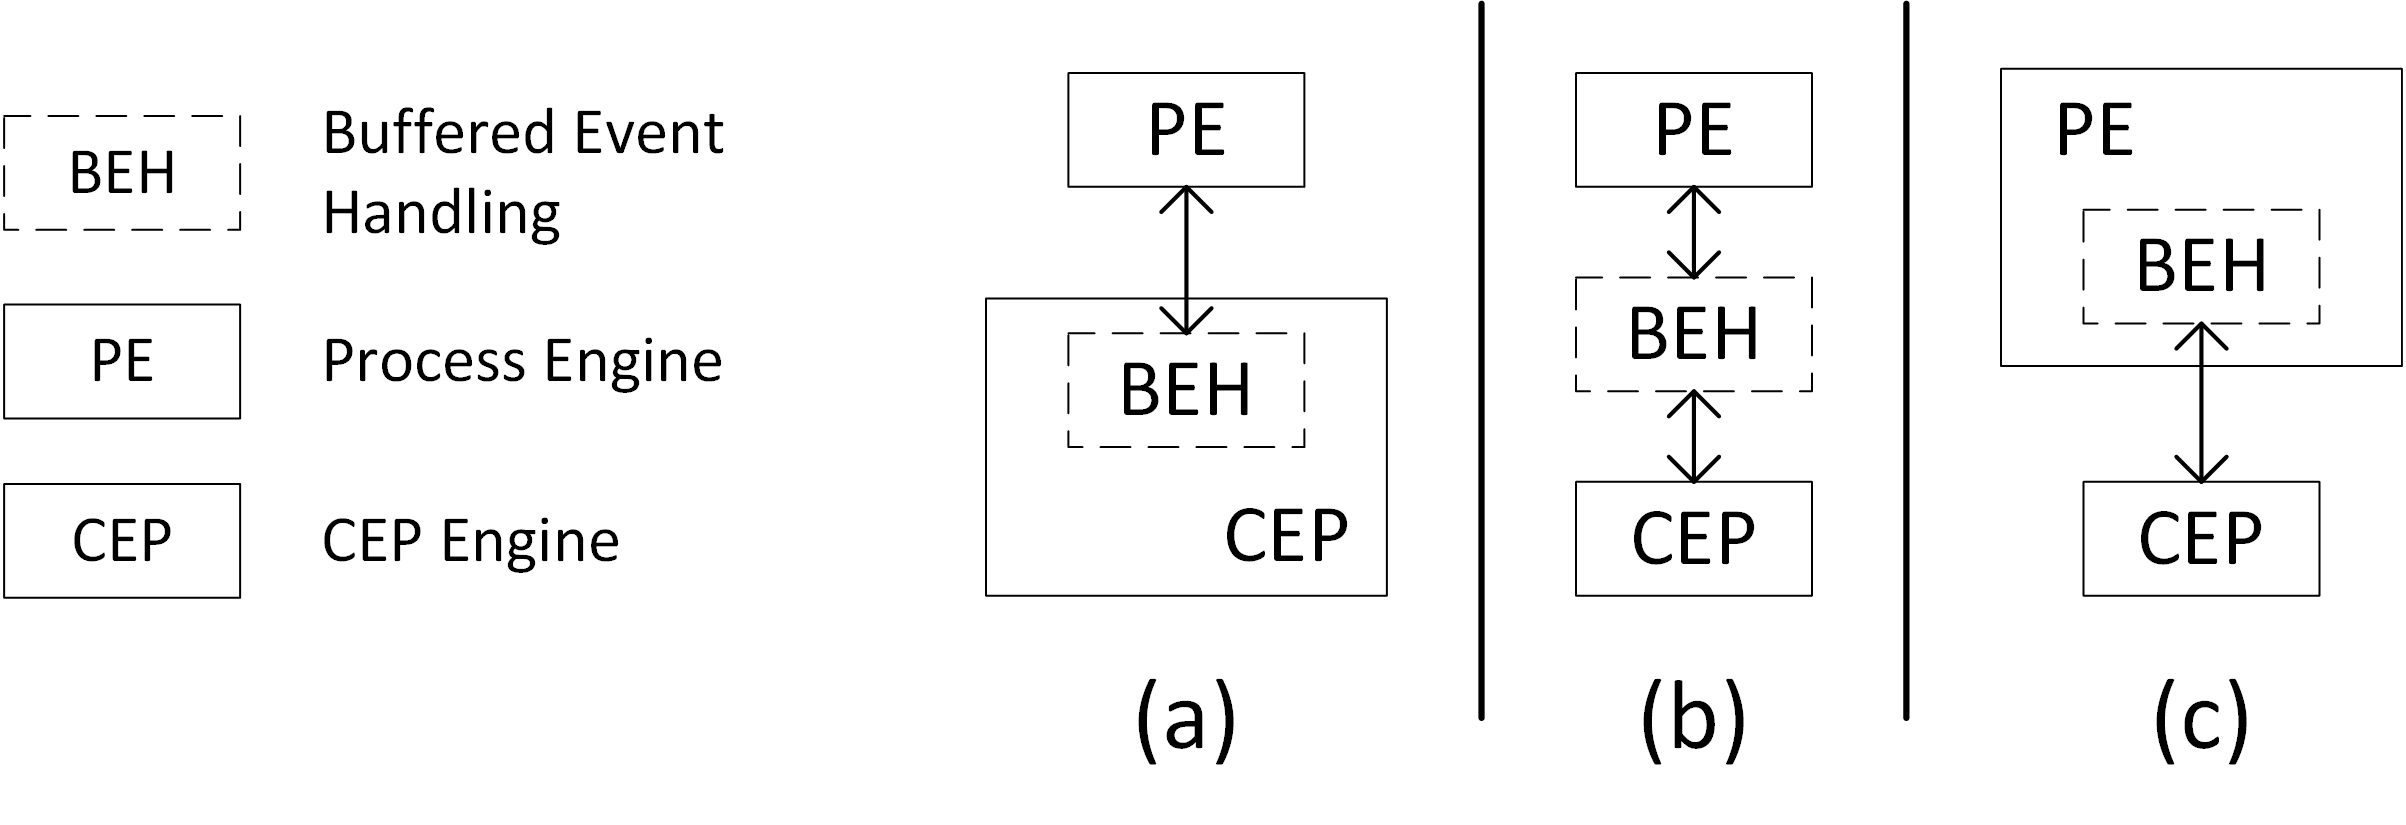
\includegraphics[width=0.8\linewidth]{chapters/concept/automaticsubscription/architecture-options.png}}
	\caption{Architectural options to implement the event buffers}
	\label{fig:buffered-event-handling-architecture}
\end{figure}

A reference implementation for an extended complex event processing platform is presented in \autoref{ch:implunicorn} at the example of the Esper-based CEP~platform \textit{Unicorn}. It also explains, why extending the event platform was the preferred choice in the given scenario.

\medskip \noindent
- given the extended api, it is now possible to implement early event subscription from the process engine
\todo[inline]{connector}


\subsection{Extended Process Engine Behavior}\label{ch:extendedprocessengine}
It is the task of the Business Process Engine to interpret and execute process models and connect to an event processing platform in event-driven setups.
From the three relevant parts, two have already been defined, the BPMN extension and the buffered event processing module.
Out of the box, a process engine like Camunda will ignore any proprietary BPMN extensions and the subscription to an event source must be especially implemented. An example for such an implementation is provided in \autoref{ass:model:buffered}.
One goal of this work is to automatize the handling of event subscriptions solely based on the information available through the extended BPMN model. Additional process elements should not be required.
This section will clarify, which operations need to be executed by the process engine to enable the automatic subscription handling.
\autoref{ch:implcamunda} demonstrates the implementation of automatic subscription handling at the example of Camunda.

\paragraph{Parsing additional information from the BPMN model}
It is required that the process engine is able to read the additional information from the BPMN extension~(see~\autoref{ch:bpmnx}) so that it is available during process deployment and execution.
This affects the BPMN message element, which can contain the additional attributes \textit{eventQuery}, \textit{subscriptionTime} and \textit{bufferPolicies}.
Secondly, the \textit{Event Subscription Task} has to be processed. It contains a reference to a Message entity within the same model element.
The process engine might have to be adopted to read all relevant data from the extended model.


\paragraph{Managing subscription and un-subscription}
As defined in the BPMN extension for flexible event subscription, the action of subscribing to an event source can happen at different times during process deployment and execution. The options and the implicit timing of subscription and un-subscription are specified in \autoref{ch:bpmnx:subscriptiontimes}.
The process engine must communicate with the process engine using the four calls \textit{registerQuery}, \textit{requestEvents}, \textit{unsubscribe} and \textit{deleteQuery}, that were presented in the previous chapter.
For each possible subscription time, the following briefly enumerates which operations must be executed when. 

\begin{description}
	\item[In every case:] 
		The return-value of \textit{registerQuery}, a unique identifier of that query, must be stored for the related BPMN \textit{Message}. The id is later necessary to execute the other three API methods.
		If the event query contains one or more variable values (see \autoref{ch:bpmnx:variables-in-queries}), all have to be replaced by their current values when \textit{registerQuery} is performed.
		When an event element is reached, a call to \textit{requestEvents} must be issued. When the execution of that event element is finished, call \textit{unsubscribe}.
	\item[Subscr. on process deployment:]
		When a process gets deployed, the process engine must check if subscription information is in the model. For every \textit{Message} element that is set as \textit{subscribe on pr. deployment}, a call to \textit{registerQuery} must be issued as part of the deployment process. A call to \textit{deleteQuery} is executed when the process gets un-deployed for the same messages.
	\item[Subscr. on process instantiation:] 
		When a process gets instantiated, \textit{registerQuery} must be executed for each \textit{Message} that is set to \textit{subscribe on pr. instantiation}. \textit{deleteQuery} can be called when the last reachable event element for a \textit{Message} has finished executing or no connected event can be reached anymore. The deletion happens at the latest when the process instance terminates.
	\item[Subscr. through explicit subscription task:]
		If the control flow reaches a subscription task, the process engine executes \textit{registerQuery} for the referenced \textit{Message}. The execution of \textit{deleteQuery} follows the same rules as in the preceding case.
	\item[Subscr. when the event element is reached:]
		Once the event element is reached, \textit{registerQuery} must be executed for any \textit{Message} that is not covered by one of the prior cases. \textit{deleteQuery} must be called when the event element is finished.
\end{description}
\todo[inline]{be more precise about the time the calls should be executed (if possible). "reached"? "completed"? use the right bpmn words}



\todo[inline]{write conclusions that repeat how each requirement has been fulfilled}

\section{Design Decicions}\label{ch:designdecisions}

The target functionality of the BPMN extension was clearly defined by the identified requirements.
To implement that functionality, there were a number of options to consider and design decisions to make.
This chapter provides background information on the decisions that have influenced the presented concept for flexible event subscription.

\todo[inline]{Talk about an alternative solution? Table of events for a certain event source. The buffer is already there for me to pick from when designing the process.}

\paragraph{The time of subscription is a question of process design}
-> process designer
- this is why the bpmn extension is presented first
- hide complexity from the designer

\paragraph{The actual buffer is mostly hidden from the user}

- Buffers are implicitly defined through the BPMN model
- keep the look and feel of the message catch event
- minimal changes to existing models, backwards compatibility

\paragraph{Avoid additional user interfaces}
- the user will only use the bpmn model
- we don't want any other element because of complexity
- the process should be self-contained, contain all necessary information for subscription and buffering.
-> single point of contact

\paragraph{Buffers are closely linked to process models}
Messages are only buffered as soon as they are explicitly required by a model
- we don't just buffer n messages because we might need them in the future. That would be a fuzzy, incalculable performance overhead.
- instead we keep as little as possible in the buffer

\paragraph{The BPMN Extension is based on the Message element}
- if I want to talk about related work that goes another way
- why are the policies a parameter of the message and not the catch event element?

\paragraph{reuse existing technology}
-> we assume that a cep is present and that basic features of event queries can be used
- if not present, then only very basic buffer functionality is available
- but we dont want to start designing another event processing layer with duplicated functionality

\cleardoublepage%************************************************
\chapter{Reference Implementation}\label{ch:implementation}
%************************************************

\autoref{ch:flexibleeventsubscription} has presented a concept that involves the model layer, the process engine and the event engine.
It enables flexible event subscription in BPMN to overcome the issues revealed in \autoref{ch:problemstatement}.
The model extension is described in \autoref{ch:bpmnx}, and allows to create BPMN models that contain all information necessary to to issue event subscriptions for the employed event elements.
To evaluate the results we enhance the business process engine Camunda and the event processing platform UNICORN following the procedures described in \autoref{ch:extendedprocessengine} and \autoref{ch:bufferedcep} respectively.
Camunda is extended by providing a Process Engine Plugin (\autoref{ch:implcamunda}), Unicorn by adapting the source code (\autoref{ch:implunicorn}).
\autoref{fig:architecture-camunda-unicorn} shows an overview of the applied architecture with added and modified elements highlighted in gray.

\begin{figure}[]
	\myfloatalign
	{\hspace*{-2.3cm}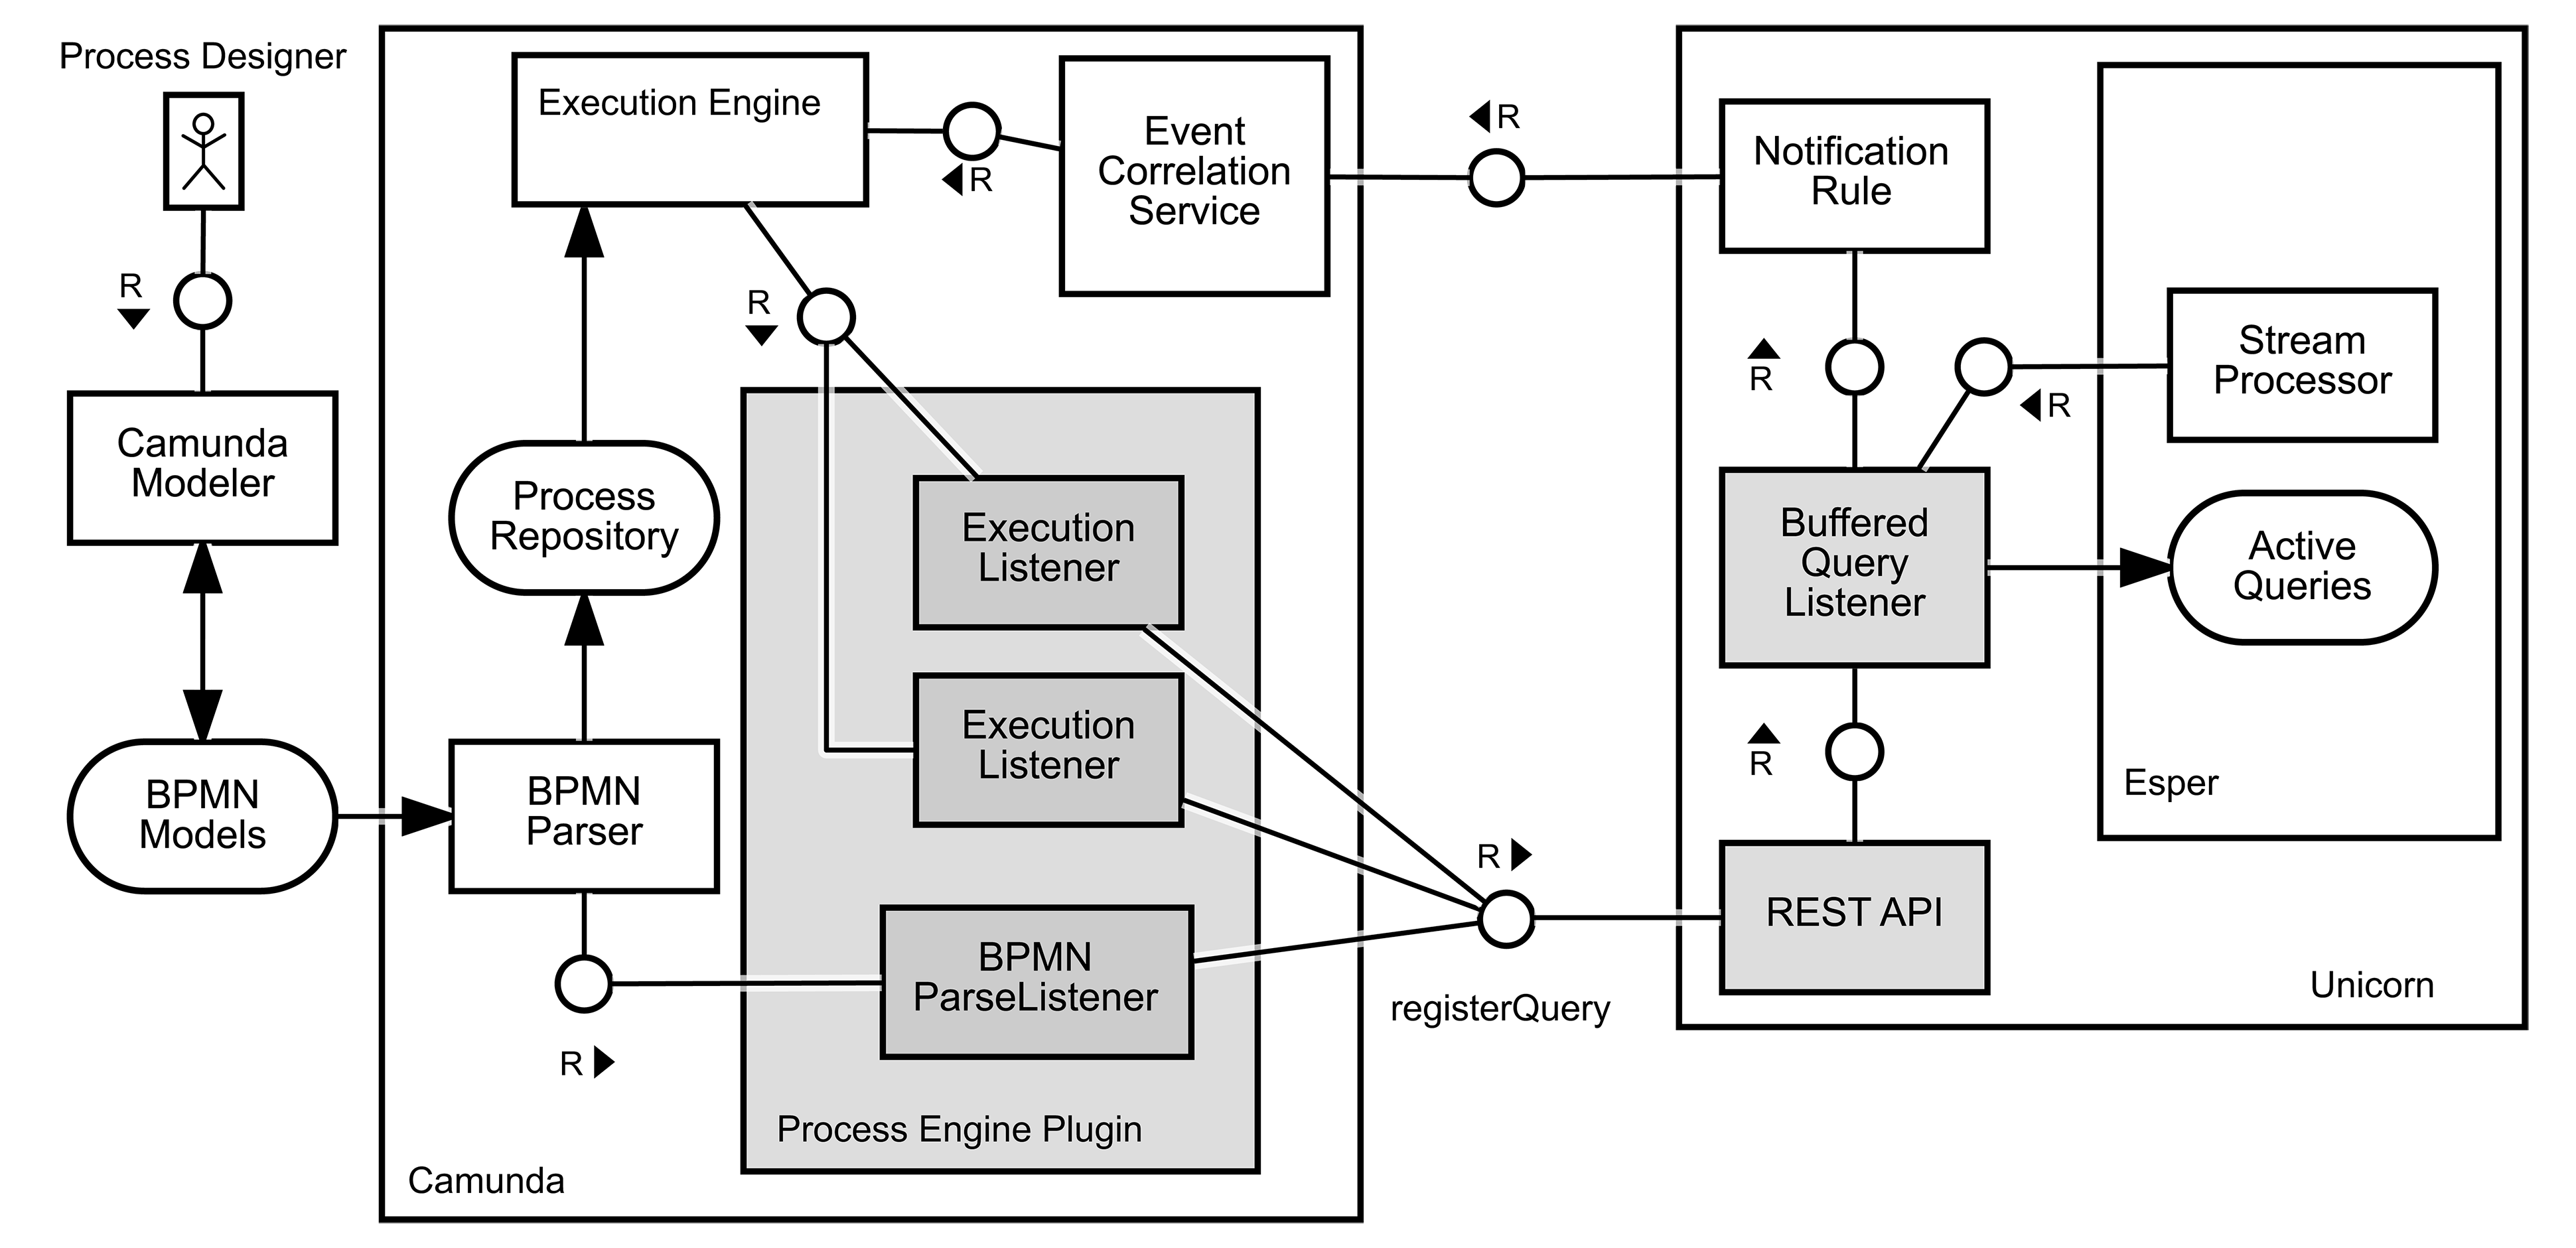
\includegraphics[width=1.3\linewidth]{chapters/implementation/flexible-evt-subscr-camunda-unicorn.png}}
	\caption{Architecture for flexible event subscription in Camunda and Unicorn}
	\label{fig:architecture-camunda-unicorn}
\end{figure}


\section{Extending the Event Processing Platform Unicorn}\label{ch:implunicorn}
\textit{UNICORN} is an event engine developed for academic purposes at the Business Process Technology chair of the Hasso-Plattner-Institute, Potsdam \cite{unicornhome, baumgrass2015get}.
%It focuses on event processing for \acs{BPM}
It has been developed in the course of the EU \textit{GET project} \cite{getservicehome}, which investigates options to increase efficiency in logistics.
Unicorn is based on the Esper \cite{esperhome}, an open source component for complex event processing available in Java.
Esper can be integrated into custom applications using its feature-rich Java API and will provide stream processing capabilities including an own \acf{EPL}.
Unicorn integrates Esper and adds a web-based user-interface, a REST API, a persistent data-store for events and a number of features specifically related to BPM.
The latest version of Unicorn uses Esper $5.3.0$, therefor all future considerations are made based on the documentation of that version.

\autoref{ch:bufferedcep} considers three architectural options to provide buffered event handling capabilities.
It has been decided to extend the event engine in this scenario for several reasons.
Firstly, the performance and operation of the process engine shall not be jeopardized (see shortcoming \textit{S3} in \autoref{ch:ass:discussion}). Event Processing features potentially require a lot of performance to handle a large number of requests in a short amount of time.
By implementing the event Buffering module loosely coupled to the Process Engine, we ensure that its performance is not influenced.
Implementing a separate middleware was avoided in the course of this work, to keep the architecture easy and concise to describe.
Unicorn is an academic prototype in constant development and therefor predestined to be directly extended for this kind of use-case.
Moreover, the chosen architecture promises performance advantages thanks to running the event buffering in the same \acs{JVM} as Esper.


\subsection{Event Buffering}
To allow the delayed delivery of events, buffering functionality is added to Unicorn.
Whereas, originally, events that match a certain query in esper are directly forwarded to the notification-recipients, they will instead be held in a buffer until requested by recipient. 
If a recipient is already subscribed, than the behavior will be equivalent to the original scenario, because the event will be delivered instantly.

\paragraph{Engine-specific Implementation Options}
When investigating the options for implementing event buffers in UNICORN, solutions that are specific to the event processing platform were considered.
Notably, the concept of a \textit{Window} in event processing languages is very much comparable with a buffer as described in this work. Windows hold a variable number of events in memory according to specified window properties. That way, windows can act like size- or time-oriented buffers and allow access to older events whenever a new event occurs.
\textit{Named Windows} in Esper allow to create global data windows that can be modified and read from multiple statements. Similar functionality is provided by \textit{Tables}, which follow a relational approach by primary key.
\footnote{see \textit{Chapter 6. EPL Reference: Named Windows And Tables}, \url{http://www.espertech.com/esper/release-5.3.0/esper-reference/html/nwtable.html}, accessed 2017-08-12}

If a query window is connected with the Esper-specific \textit{Output Clause}, it is possible to delay query output with timing constraints or trigger it on the change of a global variable.
\footnote{see \textit{Chapter 5. EPL Reference: Clauses}, \url{http://www.espertech.com/esper/release-5.3.0/esper-reference/html/epl\_clauses.html}, accessed 2017-08-12}
When putting together these features, an event buffer could be implemented as follows: The call \textit{registerQuery} instantiates the window. If the \textit{Consume}-policy is used, we use a named window that we share among queries and delete from after receiving the event. 
At \textit{subscribe}, a notification-recipient is added to a query and output is triggered by causing a variable change in Esper. \textit{Unsubscribe} and \textit{removeQuery} remove a notification-recipient and de-register the query respectively.

A major drawback of this approach is, that the event queries have to be adopted to use the specific features which makes additional knowledge necessary when designing the processes.
Alternatively, the original queries submitted by the process engine can be transformed before registering them in Unicorn, for example by encapsulating them in a sub-query. That way they make use of the mentioned features, but certain expressions will not be possible anymore due to limitations of the Esper EPL with regards to sub-queries.

Apart from this approach, it is worth noting that Unicorn offers a persistent storage of historic events, which can theoretically be used to implement the buffering functionality.
However it would be necessary to abuse the relational approach to implement a persistent stream buffer on top of the SQL database, which is not desirable.

\paragraph{The Generic Buffering Solution}
The investigation of engine-specific solutions did not bring up an optimal solution to implement an event buffer with existing mechanisms.
Furthermore, this reference implementation should not be entirely limited on one specific event engine.
For that reason a new generic buffering module has been implemented within Unicorn. 
%A \acs{UML} class diagram is provided in \autoref{}.
%\missingfigure{UML class diagram of: BufferedLiveQueryListener extends LiveQueryListener, BufferManager (list<EventBuffer> | createBuffer, updatebuffer, deleteBuffer) implements runnable, EventBuffer (Policies | update, maintain, retrieve), Constants}

The module is built around the \textit{EventBuffer}-class. Objects of the class are managed by the \textit{BufferManager} and represent a single buffer entity, holding events of one query. Esper provides the query output as an object of type \textit{EventBean}, which is stored in a list in \textit{EventBuffer}.
The buffer behaves according to the value of its policies, which influence the length of the list, the order in that items are retrieved from the buffer and the consumption behavior.
The lifetime-policy, which requires that events are deleted from the buffer after a certain time, is ensured by a maintenance-thread that runs from the BufferManager class and iterates over all EventBuffer objects in a specified time interval. The default value is 5~seconds.

Unicorn uses the \textit{LiveQueryListener} to react on new event-occurrences. It implements the Esper \textit{UpdateListener}-interface and is registered in Esper as callback-function for a new query. Whenever an event matches that query, the object of \textit{LiveQueryListener} is notified.
Originally, the QueryListener notifies all notification-recipients that are known for that query and then drops the event.
For the event buffering, a new class \textit{BufferedLiveQueryListener} is created which extends the behavior of the standard query listener. Instead of only notifying all recipients, it also updates the associated buffer instance with the latest query output.
The provided implementation serves for demonstration and reference purposes. It is not optimized for performance, for example in the case of overlapping data between buffers. Considering an event subscription issued on process instantiation, multiple \textit{EventBuffer} instances will essentially store the same data, if multiple instances of the process are started at the same time or with minimal difference.

The presented buffering module supports the temporary storage of query results as demanded by the BPMN extension. After query creation, matching events can be stored in a buffer to be retrieved when necessary.
All buffer policies described in \autoref{ch:bpmnx:bufferpolicies} have been implemented.
The following section explains how the \acs{REST}~\acs{API} of Unicorn is extended to make use of the buffering module.

\subsection{REST API Extension}\label{ch:impl:unicorn-api}
Unicorn offers a webservice that allows users to interact with the event processing engine via the \ac{HTTP}.
The restful API comprises the most basic functionality, query registration, query deletion and obtaining query strings by the subscription identifier.
An interaction generally works as follows: The user executes a POST to \textit{<platform>/EventQuery/REST}, providing an event query and information about the desired notification-recipient~(\textit{notification path}). Unicorn registers the query in Esper and returns a unique identifier to the user.
Whenever an event matches the query, the platform sends a notification to the specified recipient. a DELETE call to \textit{<platform>/EventQuery/REST/\{eventQueryUuid\}} triggers the removal of the query.

In accordance with the API requirements introduced in \autoref{ch:bufferedcep}, additional functionality has been added to the Unicorn Webservice.
The methods were added under a new path \textit{/BufferedEventQuery} to make sure that the existing features remain. They are as follows:

\begin{description}
	\item[register query]
		POST to /BufferedEventQuery, returns queryId\newline
		Payload: JSON~(eventQuery[, bufferPolicies]) with\newline bufferPolicies:(lifetime, consumption, size, order)
		
		Description: The provided eventQuery is registered in Esper using a BufferedLiveQueryListener. The BufferManager is used to instantiate a new EventBuffer object. The payload JSON object bufferPolicies is optional, and will be passed to the EventBuffer if available. Otherwise, the system falls back to the default values~(\autoref{tab:bpmn-extension}).
		A unique identifier of that query and associated buffer is returned.
	\item[subscribe]
		POST to /BufferedEventQuery/\{queryId\}\newline
		returns subscriptionId\newline
		Payload: JSON~(notificationPath) with\newline notificationPath:(notificationAddress, processInstanceId, messageName)
		
		Description: An new subscription is added to the selected query, so that a notification is issued based on the current buffer content and whenever an event matches the query.
		The notification-path is specified including the id of the target process instance and the message name. This enables Camunda to automatically correlate the issued notification to the right process execution and message.
	\item[unsubscribe]
		DELETE to /BufferedEventQuery/\{queryId\}/\{subscriptionId\}\newline
		Description: Remove the specified subscription from the list of subscriptions of the selected query.
	\item[remove query]
		DELETE to /BufferedEventQuery/\{queryId\}\newline
		Description: Remove the query and the associated buffer from the system.
\end{description}


%\paragraph{Enabling Event Correlation in Camunda}
Using instances of \textit{NotificationRule}, Unicorn sends notifications to the recipients~(see~\autoref{fig:architecture-camunda-unicorn}). In our scenario, the messages must be sent to Camunda, more specifically to a specific process instance within the engine.
The \textit{Event Correlation Service} within Camunda is responsible for relating incoming message events to process instances. One way to enforce the correlation is by inserting the process instance identifier and the message name inside the message.
For that reason, message name and process instance id must be provided when adding a subscription in the event engine. 
Unicorn has been adopted to send notifications to Camunda including the required correlation information. A sample notification for a eurotunnel delay event is shown in~\autoref{lst:unicorn-json-notification}.
%https://docs.camunda.org/manual/7.7/reference/rest/message/post-message/

\begin{lstlisting}[caption={Example of a JSON notification sent by UNICORN},label=lst:unicorn-json-notification]
{
  "messageName":"eurotunnelDelay",
  "processInstanceId":"274a876f-aed7-4a1a-916b-e85a0c2416f7",
  "processVariables": { 
    "eurotunnelDelay":{"value":"60", "type":"Integer"}
  }
}
\end{lstlisting}

After implementing the necessary extensions to the event engine, it is the task of the process engine to connect the extended process model to the buffered event handling API.
The adaptations to the process engine are presented in the following section.

\section{Event Subscription Handling in Camunda}\label{ch:implcamunda}
%\todo[inline]{In Camunda, data objects can only be used for documentation purposes. The engine ignores them, so there is no way to set a value.}

Through the BPMN extension for flexible event subscription, the information necessary to register event queries in a CEP platform can be made available in process models.
\autoref{ch:extendedprocessengine} outlines how the business process engine must be adapted to execute the operations for subscription handling.
Camunda is an open-source business process engine with support for the latest version of the BPMN and used to exemplify the modification process. Further information about Camunda is provided in \autoref{ch:bg:bpms}.

\autoref{fig:architecture-camunda-unicorn} depicts a simplified architecure of Camunda, highlighting modifications in gray.
Our workflow for flexible event subscription mainly involves the core components, execution engine, model repository, correlation service and the Camunda modeler.

\subsection{Process Engine Plugin and ExecutionListeners}
Being a community-driven open-source project, the Camunda project offers numerous options for customizing and extending its behavior.
A core concept to trigger the execution of custom code during a process execution are \textit{ExecutionListeners}.
They can be incorporated in BPMN models using the properties window of the Camunda Modeler as demonstrated in \autoref{ch:assessment}. In that case they have a textual representation in the model file, a specification can be found in the product documentation
\footnote{\textit{Camunda BPMN Extension Elements}, \url{https://docs.camunda.org/manual/7.7/reference/bpmn20/custom-extensions/extension-elements/\#executionlistener}, accessed 2017-08-10}.

However, one of the main goals of this thesis is to provide an alternative solution to explicitly modeling the subscription, unless an explicit subscription task shall be used). Thus the additional necessity attach execution listeners to BPMN elements shall be avoided.
Instead, subscriptions shall be managed automatically by the process engine solely based on the subscription definition provided in the extended message element.
To achieve this kind of behavior, Camunda offers the concept of a \ac{PEP} to intercept significant engine operations and introduce custom code. 
By this means, execution listeners can be added programatically.
The plugin is a separate software module that implements the interface \textit{ProcessEnginePlugin}
\footnote{\textit{Process Engine Plugins}, \url{https://docs.camunda.org/manual/7.7/user-guide/process-engine/process-engine-plugins/} accessed 2017-08-10}.
It is activated by adding a \textit{plugin} entry in the process engine configuration.

\cite{mandal:2017} and \cite{Pufahl2017} have chosen to directly adapt the source code of camunda. More precisely, they propose to modify the \textit{Behavior} class of the Camunda core to execute additional code when a BPMN element starts executing.
In this work, we implement a Process Engine Plugin as it allows a clearer, more understandable approach to adopting the execution behavior. 
That holds especially when it is only necessary to execute additional operations and not modify or delete existing code.
Moreover, the PEP facilitates the re-usability across environments and different versions of Camunda.

% interface def https://docs.camunda.org/javadoc/camunda-bpm-platform/7.7/?org/camunda/bpm/engine/impl/cfg/ProcessEnginePlugin.html
% peps https://docs.camunda.org/manual/7.7/user-guide/process-engine/process-engine-plugins/


%from \autoref{ch:bpmnx:basic}
%\todo[inline]{that means that in the implementation we need additional configuration values -> implementation chapter}
%- PEP config properties: cep url

\subsection{Managing Event Subscriptions at Runtime}
The Process Engine Plugin enables us to execute custom JAVA code at predefined points during engine execution.
An entry point to the modification of the execution behavior is provided through the implementation of the \textit{ProcessEnginePlugin} interface. It allows to intercept \textit{preInit}, \textit{postInit} and \textit{postProcessEngineBuild}, that means at three different points during the engine bootstrapping.
We chose to provide a custom implementation for the \textit{preInit} method, which has an object of \textit{ProcessEngineConfigurationImpl} as parameter.
With the engine configuration available, a plethora of custom handlers, validators and listeners can be registered\footnote{Some arbitrary examples are pre-/post-deployers, event-handlers, post-variable-serializers, command-interceptors. Full list available from: \url{https://docs.camunda.org/javadoc/camunda-bpm-platform/7.7/org/camunda/bpm/engine/impl/cfg/ProcessEngineConfigurationImpl.html}, accessed 2017-08-11}.

We implement a \textit{BPMNParseListener} that is to be executed after a BPMN element finished parsing~(\textit{customPostBPMNParseListeners}).
The BPMNParseListener interface allows us to react to the parsing of single elements based on their type by making a separate method for every BPMN element available.
A helpful example for using that listener is also provided on GitHub\footnote{GitHub, \textit{camunda-bpm-examples/process-engine-plugin/bpmn-parse-listener}, \url{https://github.com/camunda/camunda-bpm-examples/tree/master/process-engine-plugin/bpmn-parse-listener}, accessed 2017-08-11}.
The BPMN extension affects the intermediate and boundary message catch event, the receive task, the explicit subscription task and can also be used to specify subscription information for a message start event.
It was attempted to utilize the separate methods of every element, but it is not possible to access the subscription information in the associated message elements from that point. Apart from the provided method arguments, the engine's \textit{RepositoryService} can normally be used to view model information, but only after the deployment was finished.  
To overcome this limitation, we implement the method \textit{parseRootElement}, to which a representation of the root element \textit{bpmn:definitions} is passed, including all message and extension elements. 
Before the content of this method is described, two more aspects need to be introduced, the \textit{SubscriptionEngine} and the \textit{ExecutionListeners}. An excerpt of the related UML class diagramm is depicted in \autoref{fig:camunda-ext-uml}.

\begin{figure}[]
	\myfloatalign
	{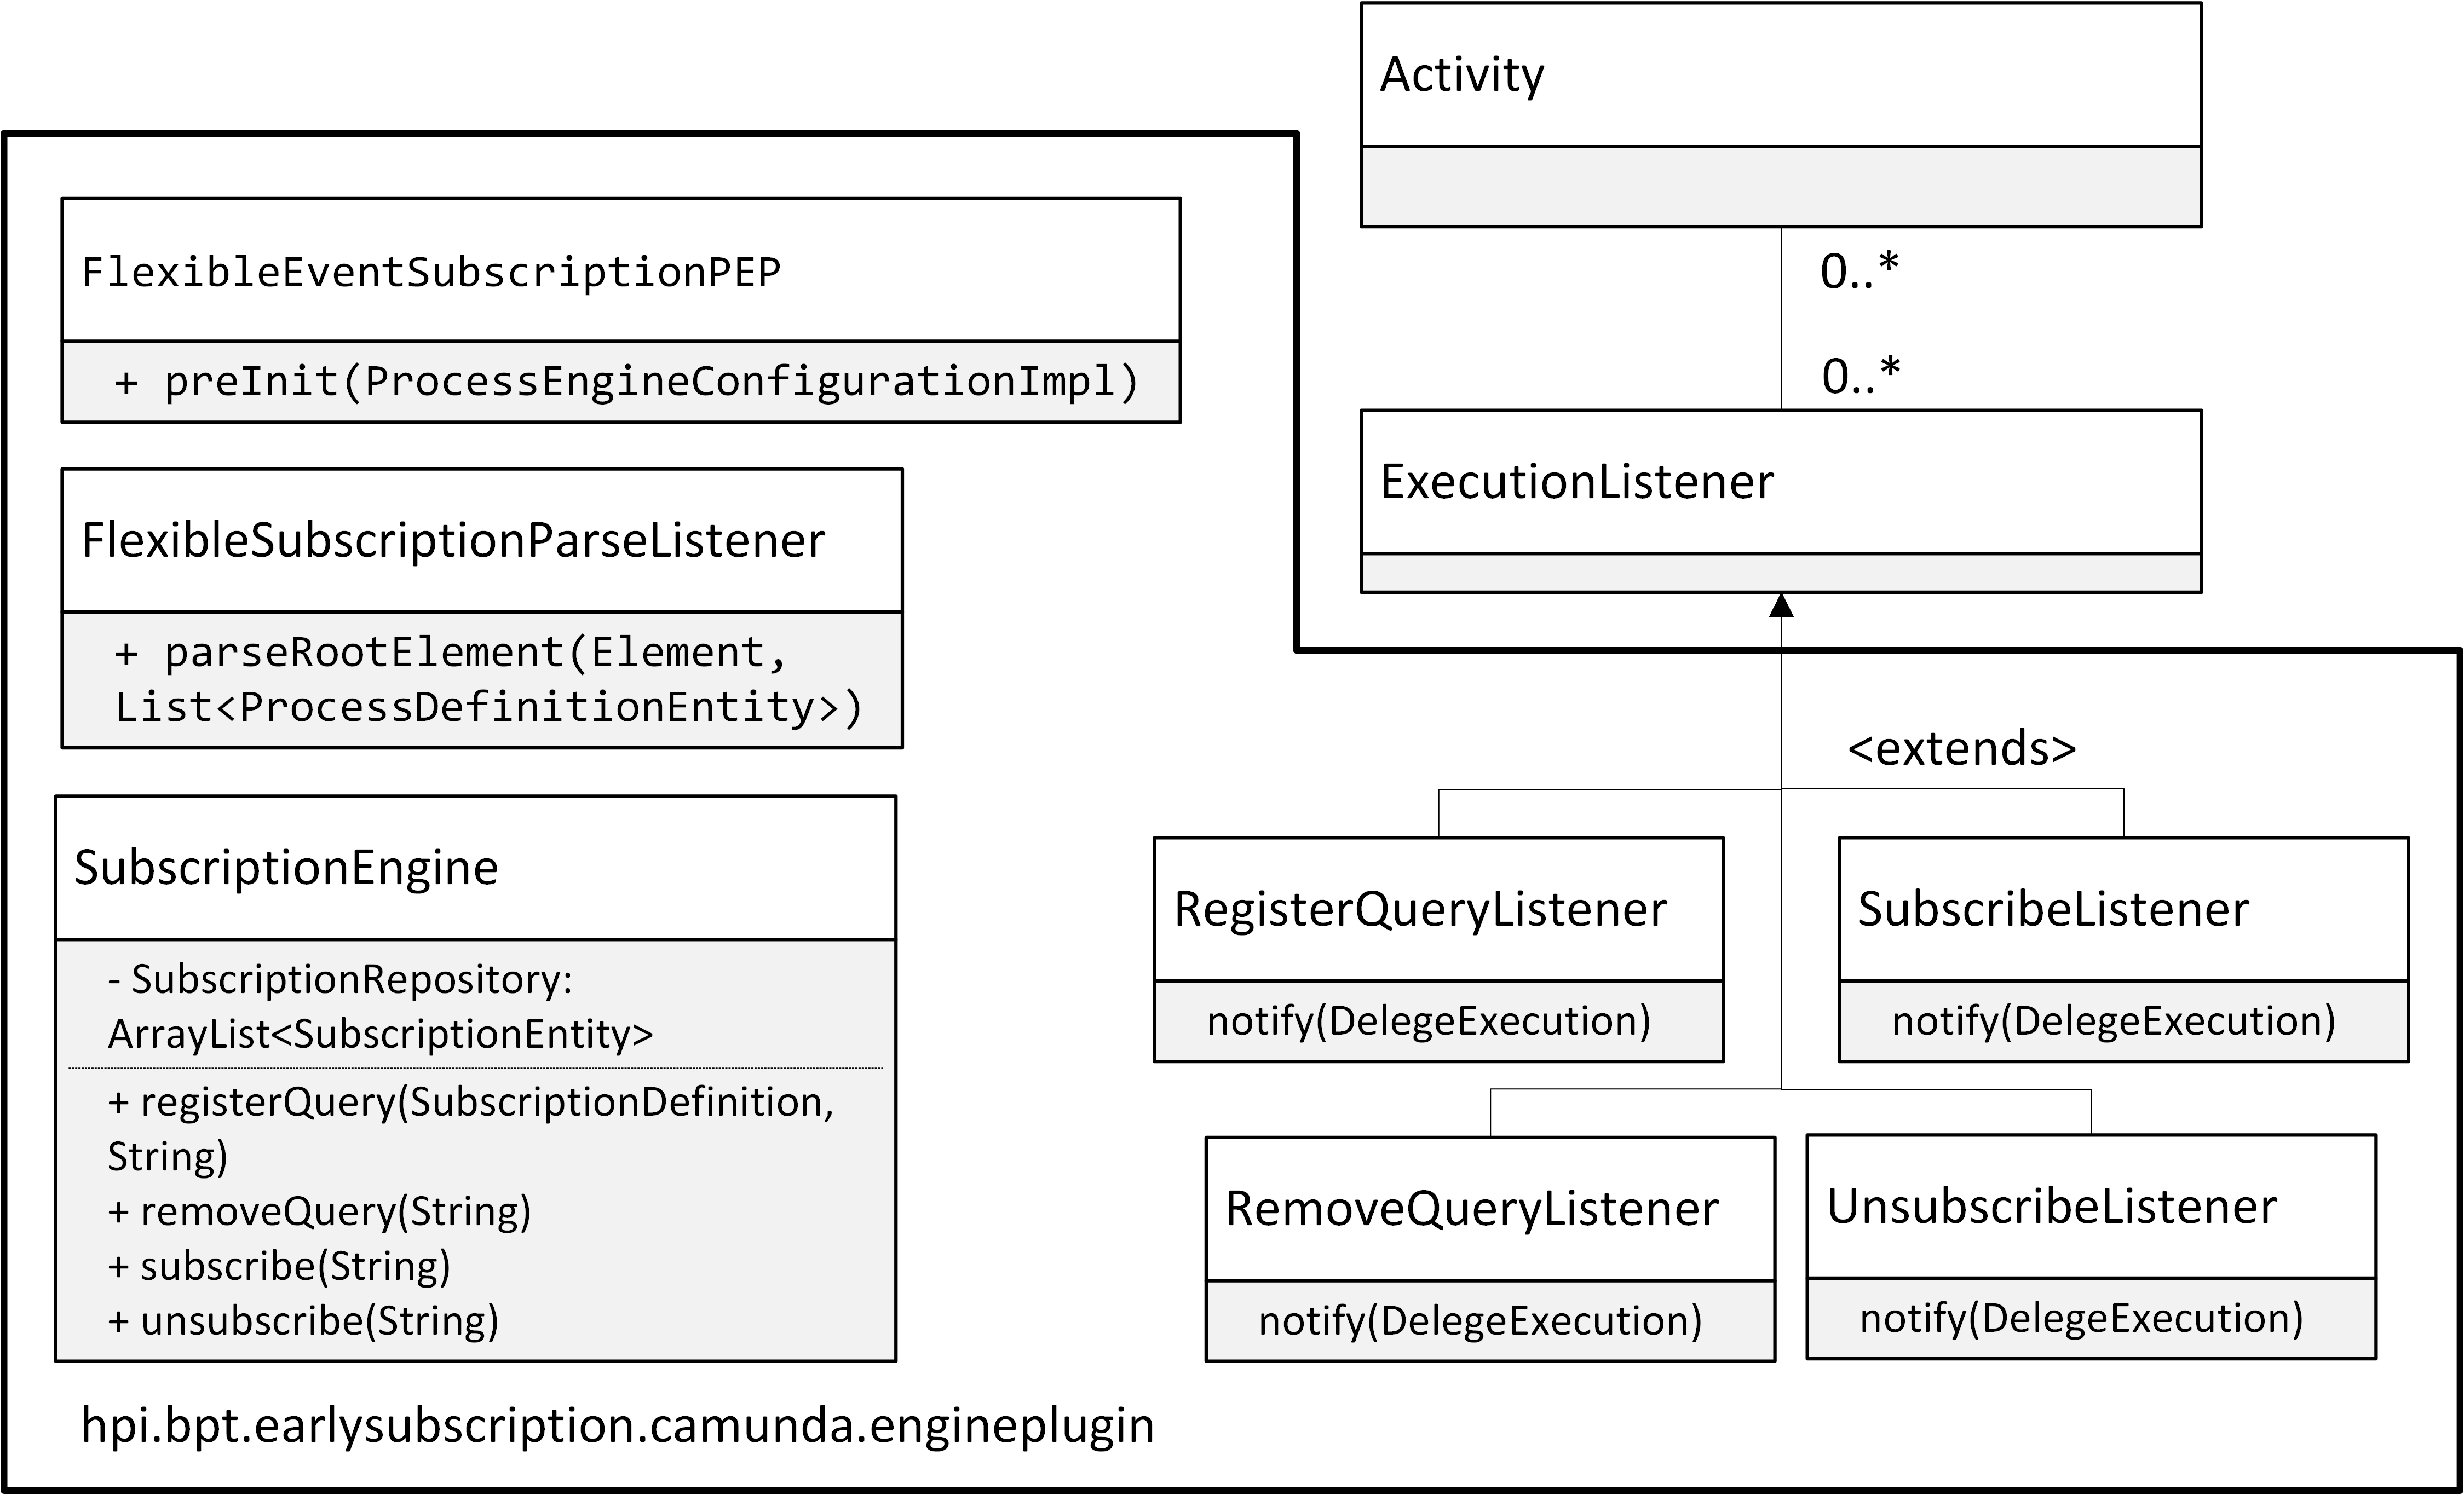
\includegraphics[width=1.0\linewidth]{chapters/implementation/uml-camunda-ext.png}}
	\caption{Excerpt of the UML class diagram of the Camunda Process Engine Plugin}
	\label{fig:camunda-ext-uml}
\end{figure}


% read a model https://docs.camunda.org/manual/7.7/user-guide/model-api/bpmn-model-api/read-a-model/
% bpmn extension elements https://docs.camunda.org/manual/7.7/user-guide/model-api/bpmn-model-api/extension-elements/

\paragraph{SubscriptionEngine}
A new class \textit{SubscriptionEngine} has been introduced, that encapsulates most of the functionality needed to communicate with the API of the event engine.
It offers method representations of all four API-calls, \textit{registerQuery}, \textit{subscribe}, \textit{unsubscribe} and \textit{removeQuery}, translating them into the according HTTP calls which are then executed.
The second, more important functionality is the \textit{SubscriptionRepository}, a list of all available query and subscription identifiers and a mapping to the related process definitions or instances.
As described in \autoref{ch:impl:unicorn-api}, active queries and subscriptions can only be deleted using their unique identifiers. 
When issuing a subscription or registering a query, these identifiers are stored in the repository until the removal call is executed.
Based on the repository information, the SubscriptionEngine can determine the subscription identifiers for provided event element information and execute the remove and unsubscribe operations on the event engine.

\paragraph{ExecutionListeners}
The concept involves four execution listeners, one for each API-call, which are attached to activities through the BPMN parse listener.
Execution listeners can be triggered by the camunda-internal end- or start-event of an activity and can therefor be used to implement the event subscription handling.
Their implementation is concise: each of them is a separate class implementing the \textit{ExecutionListener} interface. They only have one method \textit{notify}, which is called by the engine when the end- or start-event fires.
Within the method, each listener class issues an API-call using the functionality exposed by \textit{SubscriptionManager}.

%\todo[inline]{could mention that registerQuery can be bound either to an instance or to a process definition. this differentiation is made based on the subscriptionDefinition which is passed to the listener on creation.}


\paragraph{Implementation of parseRootElement}
After introducing the \textit{SubscriptionEngine} and the \textit{ExecutionListeners}, this paragraph describes how the listeners are attached to the activities in the course of the execution of \textit{parseRootElement} in our custom \textit{BPMNParseListener}.
By the help of the model representation passed ot the method as an argument of type \textit{Element}, all relevant xml~elements can be extracted based on the element names.
This results in a list of all intermediate and boundary message catch events and receive-tasks and the messages that they reference. The subscription definition is available as a child element of each message.
For each element in the list, the execution now proceeds as outlined in \autoref{ch:extendedprocessengine}.
Depending on the specified subscription time, ExecutionListeners are added at the beginning or end of activity executions or process executions. If the specified subscription time is \textit{Process Deployment}, the provided query is registered immediately using the SubscriptionManager.

This can be exemplified by an intermediate message catch event with subscription time \textit{on process instantiation}:
\begin{itemize}
	\item An instance of \textit{RegisterQueryListener} is added to the start event of the process. The \textit{subscriptiondefinition} is provided to that listener.
	\item The \textit{SubscribeListener} is attached to the start event of the activity representation of the intermediate message event.
	\item To the same activity, objects of \textit{UnsubscribeListener} and \textit{RemoveQueryListener} are registered to be triggered by the end event.
\end{itemize}

\noindent It is worth noting that the available code-base can easily be used to implement the event subscription for message start events, so that processes can be automatically instantiated by events delivered from the event engine.
Considering that process definitions in Camunda are rarely removed completely, the removal of queries on process un-deployment was not implemented. The lack of an obvious intercept point to inject code at that time makes an implementation cumbersome.

\medskip \noindent
Altogether, the enhanced CEP platform and business process engine enable the automatic handling of information provided through the BPMN extension for flexible event subscription.
The event engine exposes functionality for buffered event handling which is accessed through execution listeners during the process execution in Camunda.
The Camunda extension can be flexibly re-used across environments thanks to its implementation in the form of a Process Engine Plugin.
Given these extended features, process designers can conveniently incorporate subscription information for external message events in their executable BPMN models.




\cleardoublepage%************************************************
\chapter{Related Work}\label{ch:relatedwork}
%************************************************
\cleardoublepage%************************************************
\chapter{Conclusions}\label{ch:conclusion}
%************************************************

\section{Discussion}

- discussion:
> it remains the problem, that epl knowledge is not available in process design, a problem that has been addressed in ...
> while the event buffering can now be controlled from the process model level, events must still be acquired by the event engine before (set up event types and make sure that the events are pushed to the engine)
> the concept tries to bridge the gap between event persistence/historic events and real-time event processing by arguing that event occurrences are kept for a limited time and can therefor still be treated as events. A contra argumentation might be that an event becomes a simple piece of information as soon as it is not instantaneously consumed. hence it should not be modeled as an event but simply as a data object, using a data store
> many design decisions have been begründet with an improved usability though no empirical basis was available. Reasoning was only based on literature and chats with a small group of fellow researchers

- it can be argued that at process design time you dont care about the subscription time itself, but about the maximum age you can accept for your events. this would connect the lifetimepolicy and the subscription time into one value. but make the processing more complex and more fuzzy

\section{Future Work}


- this work attempts to provide a standard for handling event subscription in bpm architectures. given the necessity and the repeated attempts to address to topic, it would be a reasonable next step to discuss available solutions and start providing a foundation that is accepted and reused across the bpm community. No matter if based on the solutions of this work or not.
> it must be evaluated if that's the way event buffering shall be used. > prove the value of flexible event subscription in an industry case study
- future work: event data from other events could be used as historic data to allow the access even before process deployment



%\addtocontents{toc}{\protect\clearpage} % <--- just debug stuff, ignore
%\include{multiToC} % <--- just debug stuff, ignore for your documents
% ********************************************************************
% Backmatter
%*******************************************************
\appendix
%\renewcommand{\thechapter}{\alph{chapter}}
\cleardoublepage
%************************************************
\chapter{Appendix}
%************************************************

\begin{lstlisting}[basicstyle=\scriptsize,caption={XSD schema of the BPMN extension for flexible event subscription},label=lst:xsd-flexsub]
<xsd:schema xmlns:flexsub="http://www.some.url/" xmlns:xsd="http://www.w3.org/2001/XMLSchema" targetNamespace="http://www.some.url/">
<xsd:element name="eventSubscriptionTask" type="tEventSubscriptionTask" />
<xsd:complexType name="tEventSubscriptionTask">
<xsd:complexContent>
<xsd:extension base="tTask">
<xsd:attribute name="messageId" type="xsd:QName" use="required"/>
</xsd:extension>
</xsd:complexContent>
</xsd:complexType>

<xsd:element name="subscriptionDefinition">
<xsd:complexType>
<xsd:sequence>
<xsd:element type="xsd:string" name="eventQuery" minOccurs="1" maxOccurs="1" />
<xsd:element type="tSubscriptionTime" name="subscriptionTime" minOccurs="0" maxOccurs="1" default="Element Execution"/>
<xsd:element name="bufferPolicies" minOccurs="0" maxOccurs="1">
<xsd:complexType>
<xsd:sequence>
<xsd:element type="xsd:string" name="lifespanPolicy" minOccurs="0" maxOccurs="1" default="infinite"/>
<xsd:element type="xsd:string" name="consumptionPolicy" minOccurs="0" maxOccurs="1" default="Reuse"/>
<xsd:element type="xsd:integer" name="sizePolicy" minOccurs="0" maxOccurs="1" default="0"/>
<xsd:element type="tOrderPolicy" name="orderPolicy" minOccurs="0" maxOccurs="1" default="FIFO"/>
</xsd:sequence>
</xsd:complexType>
</xsd:element>
</xsd:sequence>
</xsd:complexType>
</xsd:element>

<xsd:simpleType name="tSubscriptionTime">
<xsd:restriction base="xsd:string">
<xsd:enumeration value="Process Deployment"/>
<xsd:enumeration value="Process Instantiation"/>
<xsd:enumeration value="Manual"/>
<xsd:enumeration value="Element Execution"/>
</xsd:restriction>
</xsd:simpleType>

<xsd:simpleType name="tOrderPolicy">
<xsd:restriction base="xsd:string">
<xsd:enumeration value="LIFO"/>
<xsd:enumeration value="FIFO"/>
</xsd:restriction>
</xsd:simpleType>
</xsd:schema>
\end{lstlisting}




%********************************************************************
% Other Stuff in the Back
%*******************************************************
\cleardoublepage%********************************************************************
% Bibliography
%*******************************************************
% work-around to have small caps also here in the headline
\manualmark
\markboth{\spacedlowsmallcaps{\bibname}}{\spacedlowsmallcaps{\bibname}} % work-around to have small caps also
%\phantomsection 
\refstepcounter{dummy}
\addtocontents{toc}{\protect\vspace{\beforebibskip}} % to have the bib a bit from the rest in the toc
\addcontentsline{toc}{chapter}{\tocEntry{\bibname}}
\label{app:bibliography}
\printbibliography

\cleardoublepage%*******************************************************
% Declaration
%*******************************************************
\refstepcounter{dummy}
\pdfbookmark[0]{Declaration}{declaration}
\chapter*{Declaration}
\thispagestyle{empty}
Put your declaration here.
\bigskip
 
\noindent\textit{\myLocation, \myTime}

\smallskip

\begin{flushright}
    \begin{tabular}{m{5cm}}
        \\ \hline
        \centering\myName \\
    \end{tabular}
\end{flushright}

%\cleardoublepage\pagestyle{empty}

\hfill

\vfill


\pdfbookmark[0]{Colophon}{colophon}
\section*{Colophon}
This document was typeset using the typographical look-and-feel \texttt{classicthesis} developed by Andr\'e Miede. 
The style was inspired by Robert Bringhurst's seminal book on typography ``\emph{The Elements of Typographic Style}''. 
\texttt{classicthesis} is available for both \LaTeX\ and \mLyX: 
\begin{center}
\url{https://bitbucket.org/amiede/classicthesis/}
\end{center}
Happy users of \texttt{classicthesis} usually send a real postcard to the author, a collection of postcards received so far is featured here: 
\begin{center}
\url{http://postcards.miede.de/}
\end{center}
 
\bigskip

\noindent\finalVersionString

%Hermann Zapf's \emph{Palatino} and \emph{Euler} type faces (Type~1 PostScript fonts \emph{URW
%Palladio L} and \emph{FPL}) are used. The ``typewriter'' text is typeset in \emph{Bera Mono}, 
%originally developed by Bitstream, Inc. as ``Bitstream Vera''. (Type~1 PostScript fonts were made 
%available by Malte Rosenau and
%Ulrich Dirr.)

%\paragraph{note:} The custom size of the textblock was calculated
%using the directions given by Mr. Bringhurst (pages 26--29 and
%175/176). 10~pt Palatino needs  133.21~pt for the string
%``abcdefghijklmnopqrstuvwxyz''. This yields a good line length between
%24--26~pc (288--312~pt). Using a ``\emph{double square textblock}''
%with a 1:2 ratio this results in a textblock of 312:624~pt (which
%includes the headline in this design). A good alternative would be the
%``\emph{golden section textblock}'' with a ratio of 1:1.62, here
%312:505.44~pt. For comparison, \texttt{DIV9} of the \texttt{typearea}
%package results in a line length of 389~pt (32.4~pc), which is by far
%too long. However, this information will only be of interest for
%hardcore pseudo-typographers like me.%
%
%To make your own calculations, use the following commands and look up
%the corresponding lengths in the book:
%\begin{verbatim}
%    \settowidth{\abcd}{abcdefghijklmnopqrstuvwxyz}
%    \the\abcd\ % prints the value of the length
%\end{verbatim}
%Please see the file \texttt{classicthesis.sty} for some precalculated 
%values for Palatino and Minion.
%
%    \settowidth{\abcd}{abcdefghijklmnopqrstuvwxyz}
%    \the\abcd\ % prints the value of the length





% ********************************************************************
% Game Over: Restore, Restart, or Quit?
%*******************************************************
\end{document}
% ********************************************************************
